% Generated by Sphinx.
\def\sphinxdocclass{report}
\documentclass[letterpaper,10pt,english]{sphinxmanual}
\usepackage[utf8]{inputenc}
\DeclareUnicodeCharacter{00A0}{\nobreakspace}
\usepackage{cmap}
\usepackage[T1]{fontenc}
\usepackage{babel}
\usepackage{times}
\usepackage[Bjarne]{fncychap}
\usepackage{longtable}
\usepackage{sphinx}
\usepackage{multirow}



\title{Index Insurance Sample Educational Tools}
\date{August 26, 2015}
\release{2.0.0}
\author{IRI, Earth Institute, Columbia University}
\newcommand{\sphinxlogo}{
\includegraphics{iri.pdf}\par}
\renewcommand{\releasename}{Release}
\makeindex

\makeatletter
\def\PYG@reset{\let\PYG@it=\relax \let\PYG@bf=\relax%
    \let\PYG@ul=\relax \let\PYG@tc=\relax%
    \let\PYG@bc=\relax \let\PYG@ff=\relax}
\def\PYG@tok#1{\csname PYG@tok@#1\endcsname}
\def\PYG@toks#1+{\ifx\relax#1\empty\else%
    \PYG@tok{#1}\expandafter\PYG@toks\fi}
\def\PYG@do#1{\PYG@bc{\PYG@tc{\PYG@ul{%
    \PYG@it{\PYG@bf{\PYG@ff{#1}}}}}}}
\def\PYG#1#2{\PYG@reset\PYG@toks#1+\relax+\PYG@do{#2}}

\expandafter\def\csname PYG@tok@gd\endcsname{\def\PYG@tc##1{\textcolor[rgb]{0.63,0.00,0.00}{##1}}}
\expandafter\def\csname PYG@tok@gu\endcsname{\let\PYG@bf=\textbf\def\PYG@tc##1{\textcolor[rgb]{0.50,0.00,0.50}{##1}}}
\expandafter\def\csname PYG@tok@gt\endcsname{\def\PYG@tc##1{\textcolor[rgb]{0.00,0.27,0.87}{##1}}}
\expandafter\def\csname PYG@tok@gs\endcsname{\let\PYG@bf=\textbf}
\expandafter\def\csname PYG@tok@gr\endcsname{\def\PYG@tc##1{\textcolor[rgb]{1.00,0.00,0.00}{##1}}}
\expandafter\def\csname PYG@tok@cm\endcsname{\let\PYG@it=\textit\def\PYG@tc##1{\textcolor[rgb]{0.25,0.50,0.56}{##1}}}
\expandafter\def\csname PYG@tok@vg\endcsname{\def\PYG@tc##1{\textcolor[rgb]{0.73,0.38,0.84}{##1}}}
\expandafter\def\csname PYG@tok@m\endcsname{\def\PYG@tc##1{\textcolor[rgb]{0.13,0.50,0.31}{##1}}}
\expandafter\def\csname PYG@tok@mh\endcsname{\def\PYG@tc##1{\textcolor[rgb]{0.13,0.50,0.31}{##1}}}
\expandafter\def\csname PYG@tok@cs\endcsname{\def\PYG@tc##1{\textcolor[rgb]{0.25,0.50,0.56}{##1}}\def\PYG@bc##1{\setlength{\fboxsep}{0pt}\colorbox[rgb]{1.00,0.94,0.94}{\strut ##1}}}
\expandafter\def\csname PYG@tok@ge\endcsname{\let\PYG@it=\textit}
\expandafter\def\csname PYG@tok@vc\endcsname{\def\PYG@tc##1{\textcolor[rgb]{0.73,0.38,0.84}{##1}}}
\expandafter\def\csname PYG@tok@il\endcsname{\def\PYG@tc##1{\textcolor[rgb]{0.13,0.50,0.31}{##1}}}
\expandafter\def\csname PYG@tok@go\endcsname{\def\PYG@tc##1{\textcolor[rgb]{0.20,0.20,0.20}{##1}}}
\expandafter\def\csname PYG@tok@cp\endcsname{\def\PYG@tc##1{\textcolor[rgb]{0.00,0.44,0.13}{##1}}}
\expandafter\def\csname PYG@tok@gi\endcsname{\def\PYG@tc##1{\textcolor[rgb]{0.00,0.63,0.00}{##1}}}
\expandafter\def\csname PYG@tok@gh\endcsname{\let\PYG@bf=\textbf\def\PYG@tc##1{\textcolor[rgb]{0.00,0.00,0.50}{##1}}}
\expandafter\def\csname PYG@tok@ni\endcsname{\let\PYG@bf=\textbf\def\PYG@tc##1{\textcolor[rgb]{0.84,0.33,0.22}{##1}}}
\expandafter\def\csname PYG@tok@nl\endcsname{\let\PYG@bf=\textbf\def\PYG@tc##1{\textcolor[rgb]{0.00,0.13,0.44}{##1}}}
\expandafter\def\csname PYG@tok@nn\endcsname{\let\PYG@bf=\textbf\def\PYG@tc##1{\textcolor[rgb]{0.05,0.52,0.71}{##1}}}
\expandafter\def\csname PYG@tok@no\endcsname{\def\PYG@tc##1{\textcolor[rgb]{0.38,0.68,0.84}{##1}}}
\expandafter\def\csname PYG@tok@na\endcsname{\def\PYG@tc##1{\textcolor[rgb]{0.25,0.44,0.63}{##1}}}
\expandafter\def\csname PYG@tok@nb\endcsname{\def\PYG@tc##1{\textcolor[rgb]{0.00,0.44,0.13}{##1}}}
\expandafter\def\csname PYG@tok@nc\endcsname{\let\PYG@bf=\textbf\def\PYG@tc##1{\textcolor[rgb]{0.05,0.52,0.71}{##1}}}
\expandafter\def\csname PYG@tok@nd\endcsname{\let\PYG@bf=\textbf\def\PYG@tc##1{\textcolor[rgb]{0.33,0.33,0.33}{##1}}}
\expandafter\def\csname PYG@tok@ne\endcsname{\def\PYG@tc##1{\textcolor[rgb]{0.00,0.44,0.13}{##1}}}
\expandafter\def\csname PYG@tok@nf\endcsname{\def\PYG@tc##1{\textcolor[rgb]{0.02,0.16,0.49}{##1}}}
\expandafter\def\csname PYG@tok@si\endcsname{\let\PYG@it=\textit\def\PYG@tc##1{\textcolor[rgb]{0.44,0.63,0.82}{##1}}}
\expandafter\def\csname PYG@tok@s2\endcsname{\def\PYG@tc##1{\textcolor[rgb]{0.25,0.44,0.63}{##1}}}
\expandafter\def\csname PYG@tok@vi\endcsname{\def\PYG@tc##1{\textcolor[rgb]{0.73,0.38,0.84}{##1}}}
\expandafter\def\csname PYG@tok@nt\endcsname{\let\PYG@bf=\textbf\def\PYG@tc##1{\textcolor[rgb]{0.02,0.16,0.45}{##1}}}
\expandafter\def\csname PYG@tok@nv\endcsname{\def\PYG@tc##1{\textcolor[rgb]{0.73,0.38,0.84}{##1}}}
\expandafter\def\csname PYG@tok@s1\endcsname{\def\PYG@tc##1{\textcolor[rgb]{0.25,0.44,0.63}{##1}}}
\expandafter\def\csname PYG@tok@gp\endcsname{\let\PYG@bf=\textbf\def\PYG@tc##1{\textcolor[rgb]{0.78,0.36,0.04}{##1}}}
\expandafter\def\csname PYG@tok@sh\endcsname{\def\PYG@tc##1{\textcolor[rgb]{0.25,0.44,0.63}{##1}}}
\expandafter\def\csname PYG@tok@ow\endcsname{\let\PYG@bf=\textbf\def\PYG@tc##1{\textcolor[rgb]{0.00,0.44,0.13}{##1}}}
\expandafter\def\csname PYG@tok@sx\endcsname{\def\PYG@tc##1{\textcolor[rgb]{0.78,0.36,0.04}{##1}}}
\expandafter\def\csname PYG@tok@bp\endcsname{\def\PYG@tc##1{\textcolor[rgb]{0.00,0.44,0.13}{##1}}}
\expandafter\def\csname PYG@tok@c1\endcsname{\let\PYG@it=\textit\def\PYG@tc##1{\textcolor[rgb]{0.25,0.50,0.56}{##1}}}
\expandafter\def\csname PYG@tok@kc\endcsname{\let\PYG@bf=\textbf\def\PYG@tc##1{\textcolor[rgb]{0.00,0.44,0.13}{##1}}}
\expandafter\def\csname PYG@tok@c\endcsname{\let\PYG@it=\textit\def\PYG@tc##1{\textcolor[rgb]{0.25,0.50,0.56}{##1}}}
\expandafter\def\csname PYG@tok@mf\endcsname{\def\PYG@tc##1{\textcolor[rgb]{0.13,0.50,0.31}{##1}}}
\expandafter\def\csname PYG@tok@err\endcsname{\def\PYG@bc##1{\setlength{\fboxsep}{0pt}\fcolorbox[rgb]{1.00,0.00,0.00}{1,1,1}{\strut ##1}}}
\expandafter\def\csname PYG@tok@mb\endcsname{\def\PYG@tc##1{\textcolor[rgb]{0.13,0.50,0.31}{##1}}}
\expandafter\def\csname PYG@tok@ss\endcsname{\def\PYG@tc##1{\textcolor[rgb]{0.32,0.47,0.09}{##1}}}
\expandafter\def\csname PYG@tok@sr\endcsname{\def\PYG@tc##1{\textcolor[rgb]{0.14,0.33,0.53}{##1}}}
\expandafter\def\csname PYG@tok@mo\endcsname{\def\PYG@tc##1{\textcolor[rgb]{0.13,0.50,0.31}{##1}}}
\expandafter\def\csname PYG@tok@kd\endcsname{\let\PYG@bf=\textbf\def\PYG@tc##1{\textcolor[rgb]{0.00,0.44,0.13}{##1}}}
\expandafter\def\csname PYG@tok@mi\endcsname{\def\PYG@tc##1{\textcolor[rgb]{0.13,0.50,0.31}{##1}}}
\expandafter\def\csname PYG@tok@kn\endcsname{\let\PYG@bf=\textbf\def\PYG@tc##1{\textcolor[rgb]{0.00,0.44,0.13}{##1}}}
\expandafter\def\csname PYG@tok@o\endcsname{\def\PYG@tc##1{\textcolor[rgb]{0.40,0.40,0.40}{##1}}}
\expandafter\def\csname PYG@tok@kr\endcsname{\let\PYG@bf=\textbf\def\PYG@tc##1{\textcolor[rgb]{0.00,0.44,0.13}{##1}}}
\expandafter\def\csname PYG@tok@s\endcsname{\def\PYG@tc##1{\textcolor[rgb]{0.25,0.44,0.63}{##1}}}
\expandafter\def\csname PYG@tok@kp\endcsname{\def\PYG@tc##1{\textcolor[rgb]{0.00,0.44,0.13}{##1}}}
\expandafter\def\csname PYG@tok@w\endcsname{\def\PYG@tc##1{\textcolor[rgb]{0.73,0.73,0.73}{##1}}}
\expandafter\def\csname PYG@tok@kt\endcsname{\def\PYG@tc##1{\textcolor[rgb]{0.56,0.13,0.00}{##1}}}
\expandafter\def\csname PYG@tok@sc\endcsname{\def\PYG@tc##1{\textcolor[rgb]{0.25,0.44,0.63}{##1}}}
\expandafter\def\csname PYG@tok@sb\endcsname{\def\PYG@tc##1{\textcolor[rgb]{0.25,0.44,0.63}{##1}}}
\expandafter\def\csname PYG@tok@k\endcsname{\let\PYG@bf=\textbf\def\PYG@tc##1{\textcolor[rgb]{0.00,0.44,0.13}{##1}}}
\expandafter\def\csname PYG@tok@se\endcsname{\let\PYG@bf=\textbf\def\PYG@tc##1{\textcolor[rgb]{0.25,0.44,0.63}{##1}}}
\expandafter\def\csname PYG@tok@sd\endcsname{\let\PYG@it=\textit\def\PYG@tc##1{\textcolor[rgb]{0.25,0.44,0.63}{##1}}}

\def\PYGZbs{\char`\\}
\def\PYGZus{\char`\_}
\def\PYGZob{\char`\{}
\def\PYGZcb{\char`\}}
\def\PYGZca{\char`\^}
\def\PYGZam{\char`\&}
\def\PYGZlt{\char`\<}
\def\PYGZgt{\char`\>}
\def\PYGZsh{\char`\#}
\def\PYGZpc{\char`\%}
\def\PYGZdl{\char`\$}
\def\PYGZhy{\char`\-}
\def\PYGZsq{\char`\'}
\def\PYGZdq{\char`\"}
\def\PYGZti{\char`\~}
% for compatibility with earlier versions
\def\PYGZat{@}
\def\PYGZlb{[}
\def\PYGZrb{]}
\makeatother

\renewcommand\PYGZsq{\textquotesingle}

\begin{document}

\maketitle
\tableofcontents
\phantomsection\label{index_updated_educationalMat::doc}



\chapter{CLIMATE RISK AND APPORTUNITIES}
\label{whatisindexinsurance/Climate_risk_and_opportunities_updated_intro:climate-risk-and-opportunities}\label{whatisindexinsurance/Climate_risk_and_opportunities_updated_intro::doc}\label{whatisindexinsurance/Climate_risk_and_opportunities_updated_intro:climate-risk-and-apportunities}

\section{Topic: Climate Risk and Opportunities}
\label{whatisindexinsurance/Climate_risk_and_opportunities_updated_intro:topic-climate-risk-and-opportunities}

\subsection{Introduction}
\label{whatisindexinsurance/Climate_risk_and_opportunities_updated_intro:introduction}
Agricultural productivity in developing countries is blocked by weather related risks that prevent farmers from using fertilizer and high quality seeds. Climate shocks like droughts and floods often lead to food insecurity, debt and the destruction of productive assets, such as plow animals, which can push people into persistent poverty. But even in relatively ``good'' years, the threat of climate shocks makes people and institutions unable or unwilling to make investments or to take out loans that could help to increase productivity, because a climate shock, such as a drought, could render their investments worthless. As a result, farmers are often unable to reap the full benefits of good years.

In the most basic sense, \emph{climate risk management} efforts are those that try to reduce the impacts that weather and climate extremes can have on lives and livelihoods. For example, insurance can help enhance productivity for farmers in normal years by protecting them from the risks of the worst years, providing a foundation for economic growth. Index insurance is a relatively new tool that farmers can use to help manage risk. Unlike traditional crop insurance, which pays out based on consequences of weather, such as farmer’s crop yields, index insurance pays out based on an index, such as rainfall, which can be measured at a local weather station or by satellite.  Index insurance can be integrated into a broader set of climate risk management and development tools specifically designed as a package to decrease farmers’ vulnerability to weather-related risks, improving lives and livelihoods.


\subsection{Index Insurance Game}
\label{whatisindexinsurance/Climate_risk_and_opportunities_updated_intro:index-insurance-game}\begin{figure}[htbp]
\centering

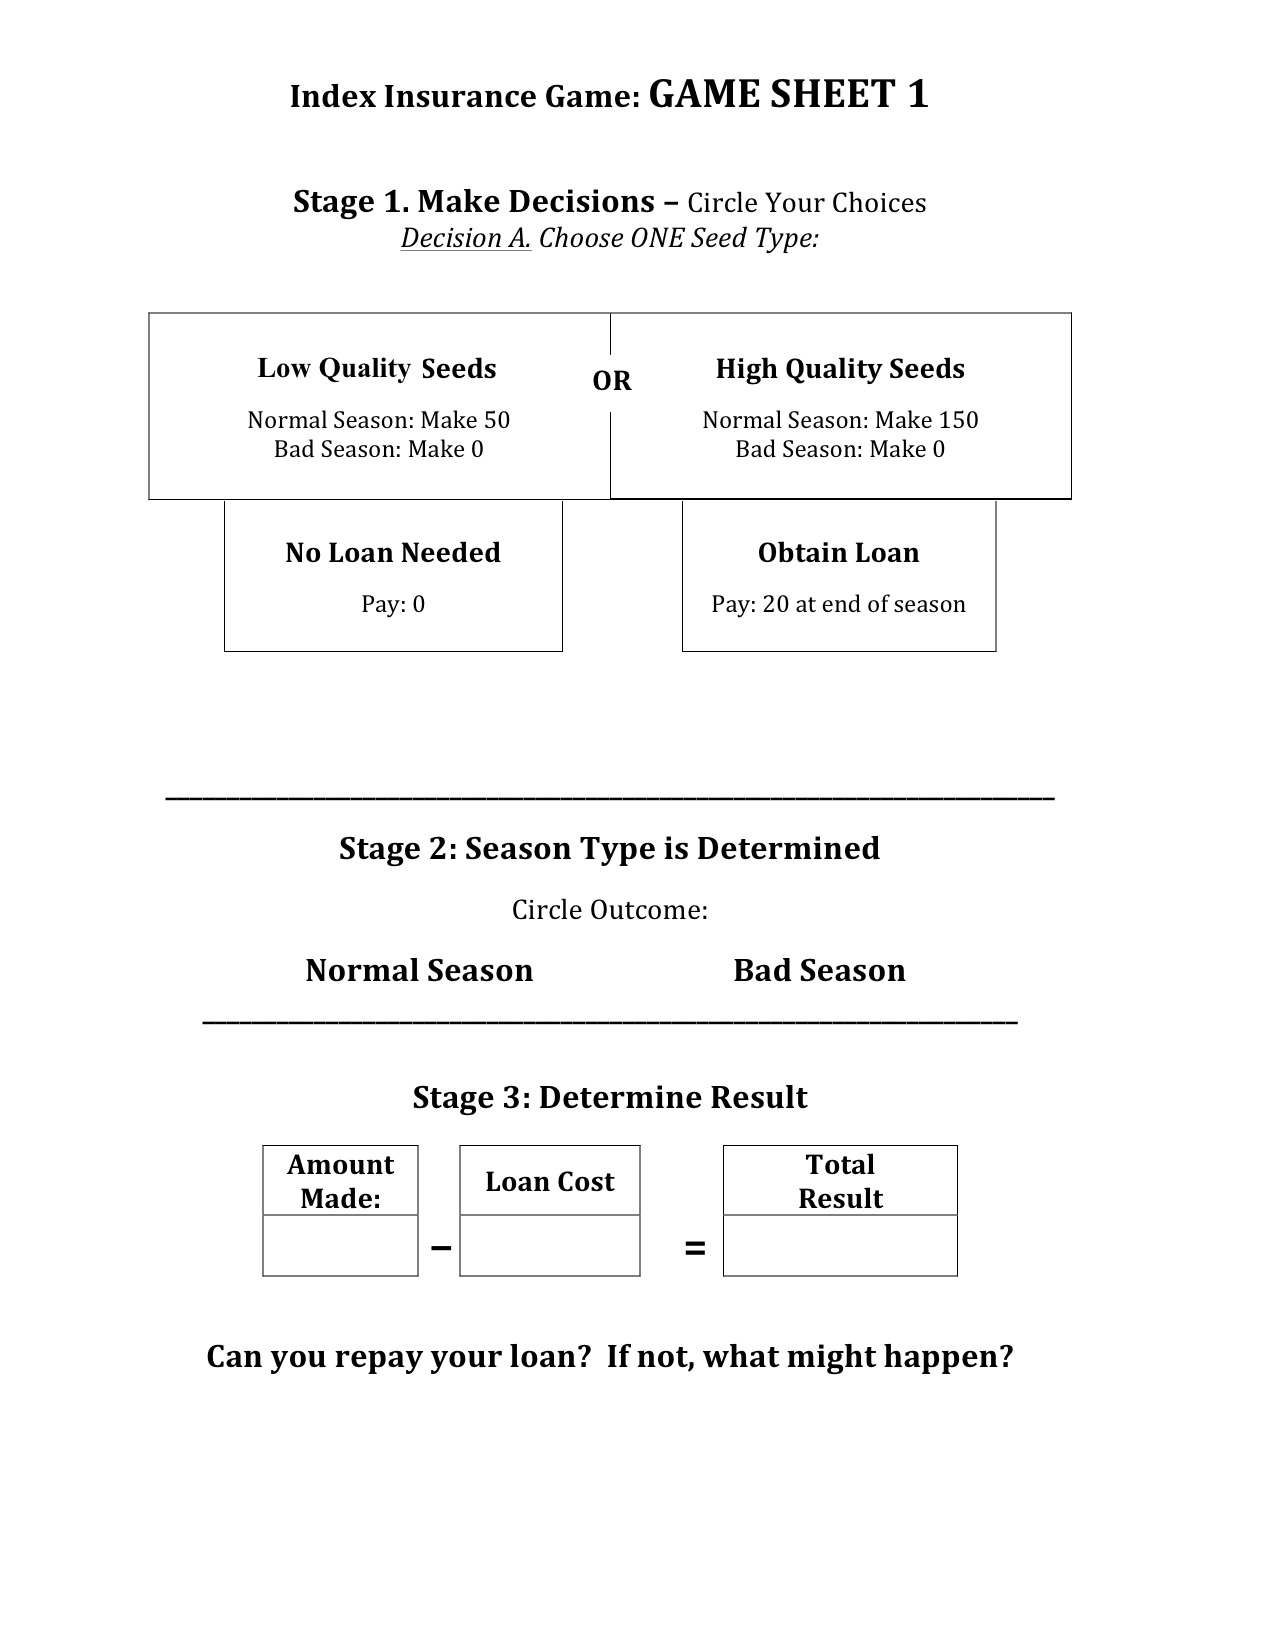
\includegraphics{indexinsurancegame1_en1.png}
\end{figure}
\begin{figure}[htbp]
\centering

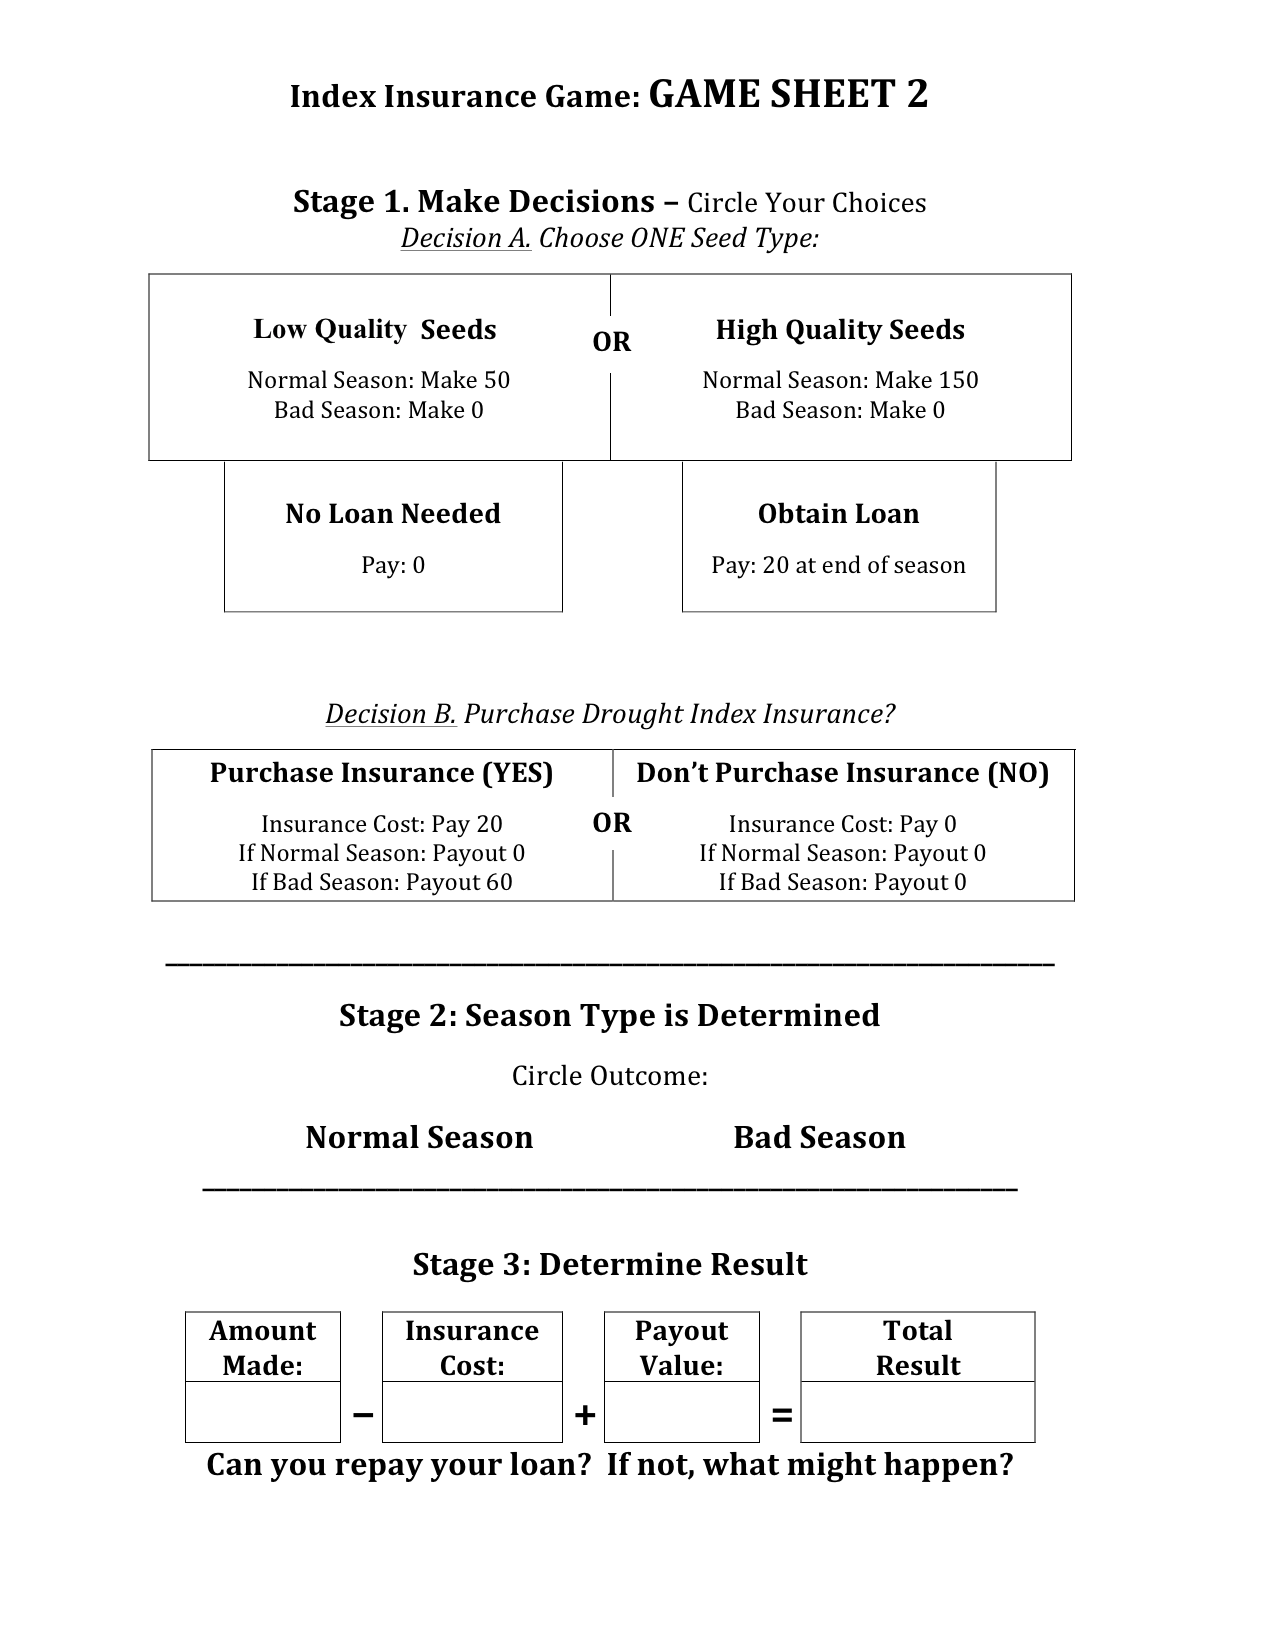
\includegraphics{indexinsurancegame2_en1.png}
\end{figure}
\begin{figure}[htbp]
\centering

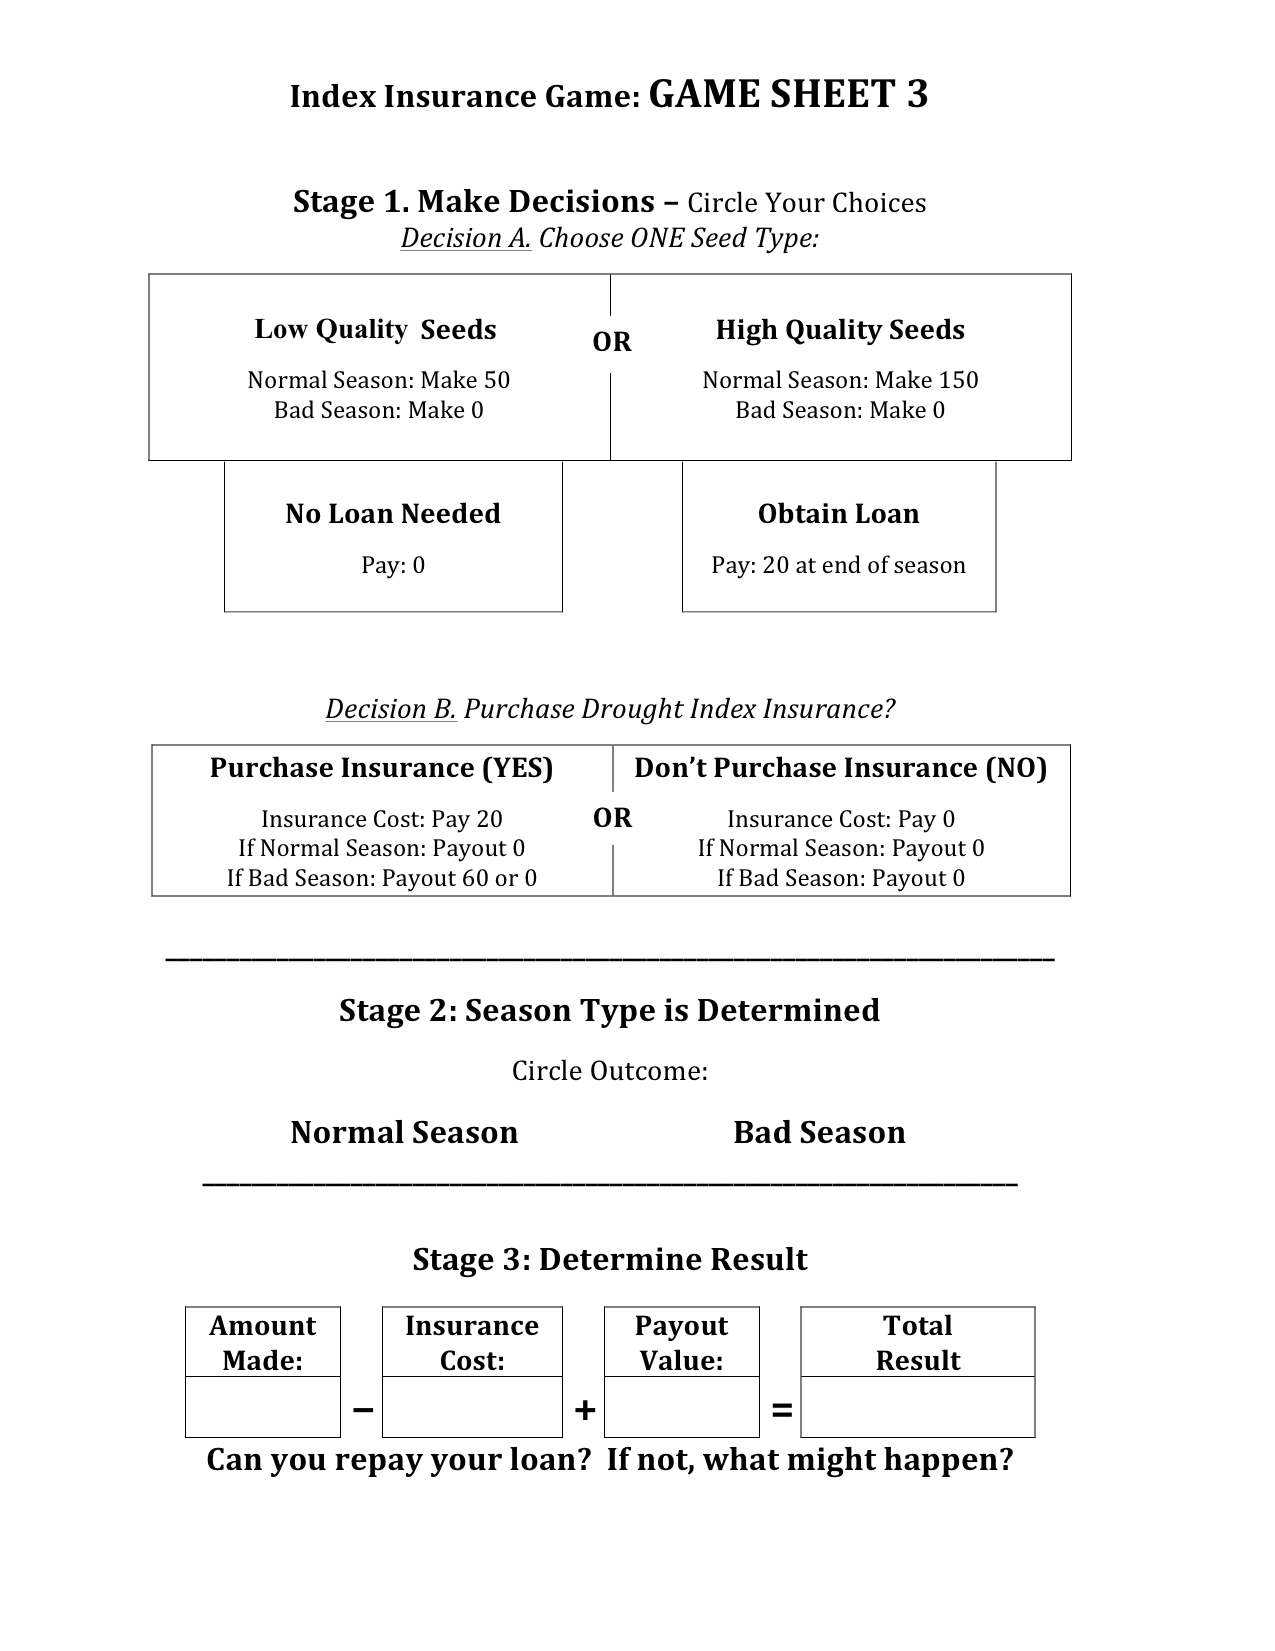
\includegraphics{indexinsurancegame3_en1.png}
\end{figure}
\begin{figure}[htbp]
\centering

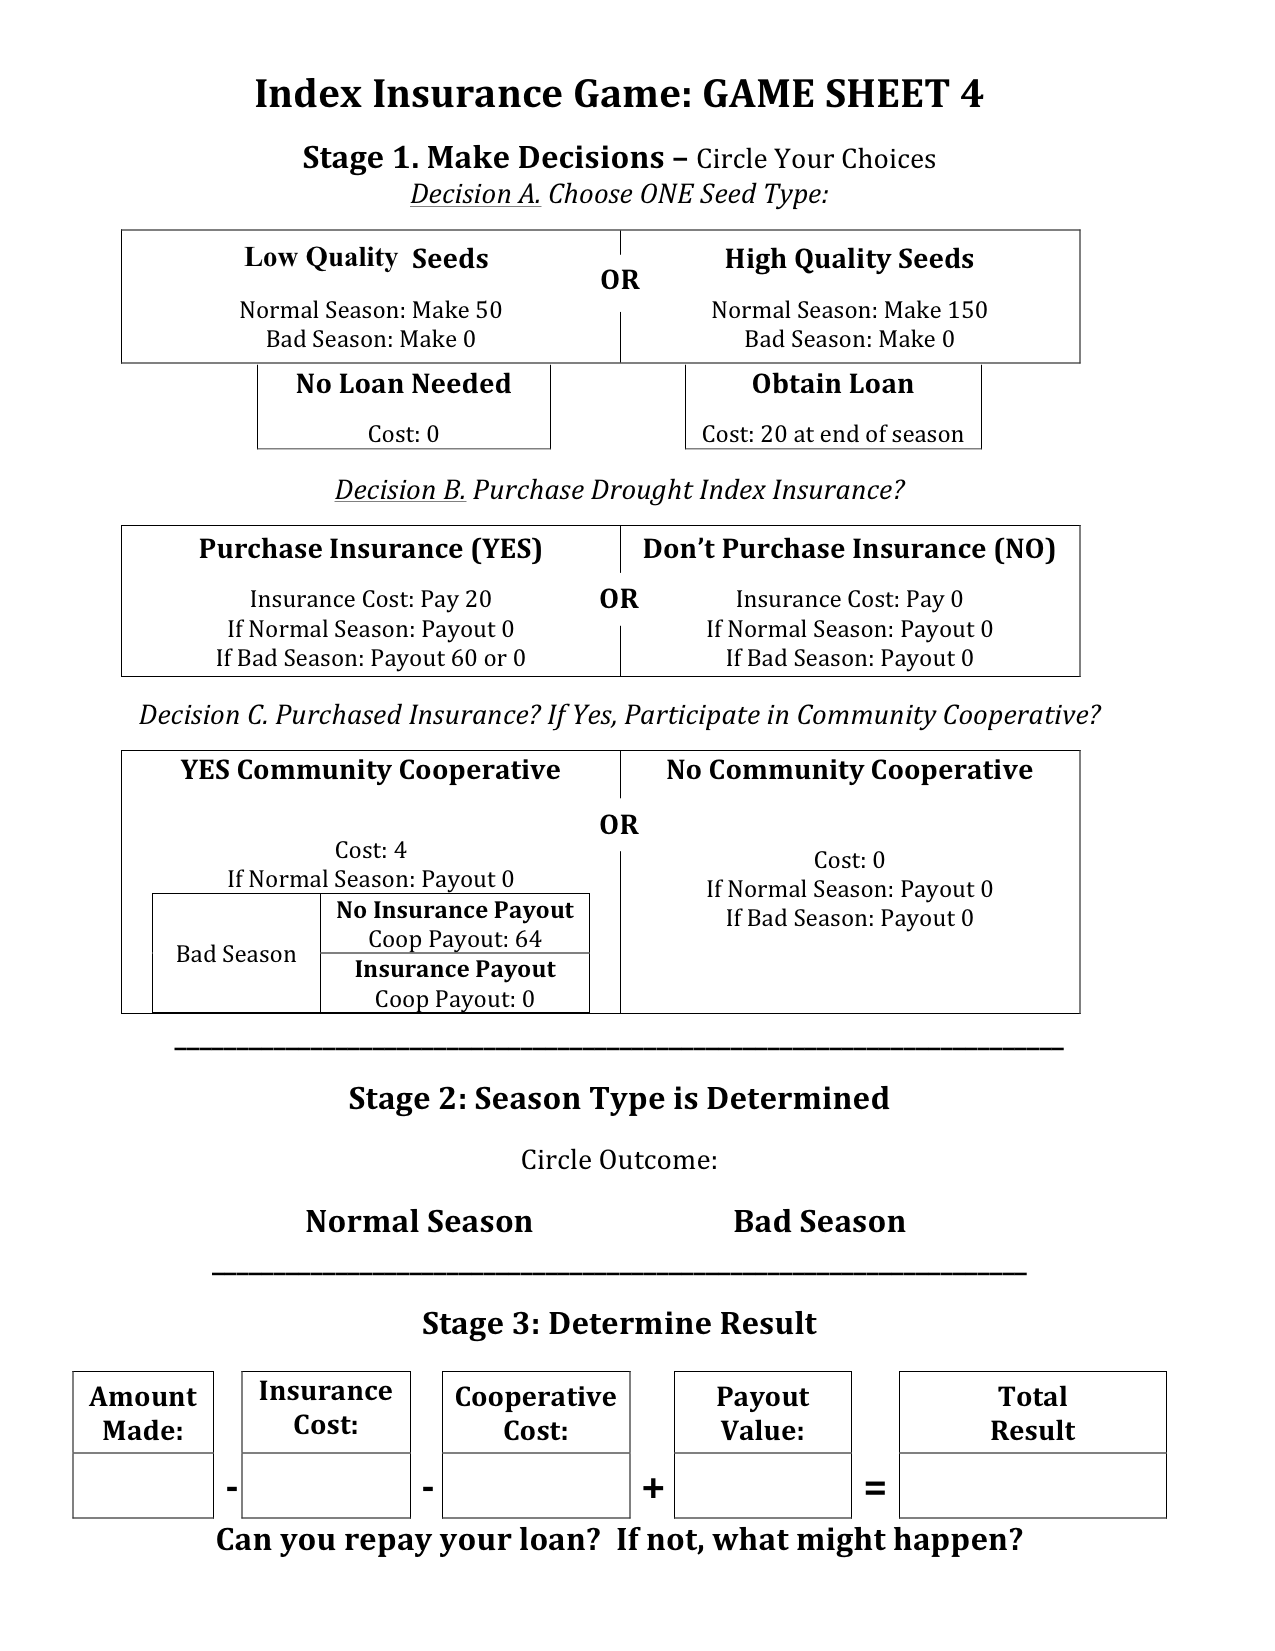
\includegraphics{indexinsurancegame4_en1.png}
\end{figure}


\chapter{OVERVIEW GAME INSTRUCTIONS}
\label{games/gameinstructions_quickreference_en:overview-game-instructions}\label{games/gameinstructions_quickreference_en::doc}

\section{Objective}
\label{games/gameinstructions_quickreference_en:objective}
This game is designed to illustrate how the decision to purchase index insurance can relate to a farmer’s input decisions for a planting season.

In this game, you are a farmer who is making input decisions for the upcoming season.  You start every phase of the game with no savings. There will be three main choices you will make before the planting season begins: what type of seed to use, to purchase insurance, and to participate in a community cooperative.

You will make these decisions before you know whether the upcoming season will be ``normal'' or ``bad''. A normal season will have sufficient rainfall to support your crop growth.  A bad season is one with low rainfall, causing drought. There is a 1-in-5 year risk of drought; in one out of every five years, you are likely to have a bad season. In order to explore all the possible outcomes, participants will play the game for several rounds. \textbf{In each round you will play the same year, you will not playing consecutive years.} The type of season is determined in Stage 2 of the game, after you have made your decisions in Stage 1.  In Stage 3 of the game, we determine your results, based on the decisions you made, and the type of season that occurred.

The facilitator should put 5 packets of gum in an opaque bag (or container, hat etc). 4 of the 5 packets of gum will be blue indicating a normal season and 1 of the 5 packets will be red indicating a bad season.


\section{List of suggested items}
\label{games/gameinstructions_quickreference_en:list-of-suggested-items}
\textbf{Documents:}
\begin{itemize}
\item {} 
1 of each of the 4 game sheets

\item {} 
facilitator instructions

\item {} 
participant instructions

\item {} 
result sheet

\item {} 
discussion points

\end{itemize}

\textbf{Supplies:}
\begin{itemize}
\item {} 
5 packets of gum - 1 packets of red gum (bad season) and 4 packets of blue gum (normal season)

\item {} 
opaque bag or container or hat

\item {} 
dice

\item {} 
markers

\item {} 
board or flip chart or larger piece of paper

\item {} 
pens and/or pencils

\end{itemize}


\section{Game Instructions}
\label{games/gameinstructions_quickreference_en:game-instructions}\begin{figure}[htbp]
\centering

\scalebox{0.500000}{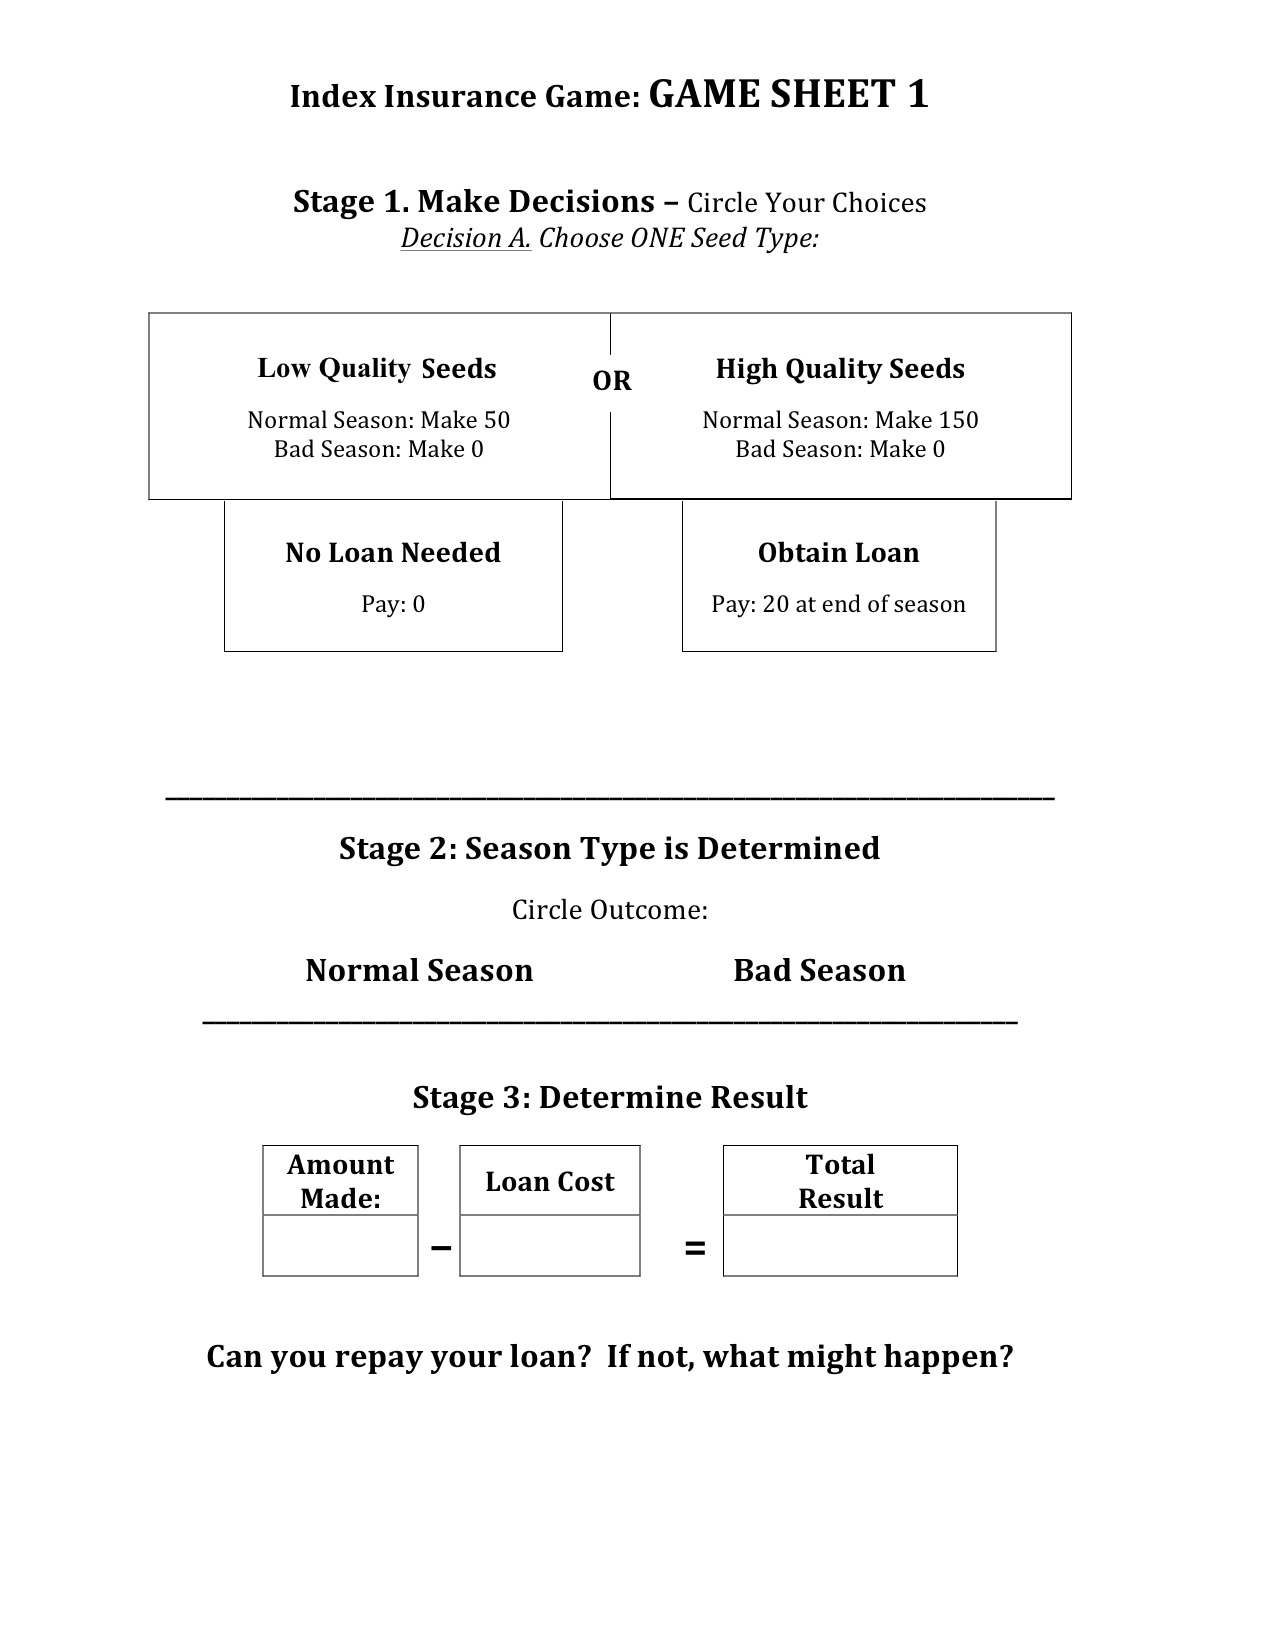
\includegraphics{indexinsurancegame1_en.png}}
\end{figure}


\subsection{Game Sheet 1}
\label{games/gameinstructions_quickreference_en:game-sheet-1}
\textbf{Instructions}

This is the first stage of the game, and should serve as an introduction. Facilitator will discuss the outcomes of each decision.

\textbf{Discussion Questions}
\begin{enumerate}
\item {} 
What would happen if you chose high quality seeds and it was a bad year? How much would you have earned?

\item {} 
How much would you earn with low quality seeds during a normal year? How much would you earn with high quality seeds during a normal year? What would you prefer and why?

\end{enumerate}

\textbf{Key Points}
\begin{itemize}
\item {} 
There are choices that help increase productivity, but they can be risky to farmers that are making decision under an uncertain climate.

\end{itemize}


\subsection{Game Sheet 2}
\label{games/gameinstructions_quickreference_en:game-sheet-2}\begin{figure}[htbp]
\centering

\scalebox{0.330000}{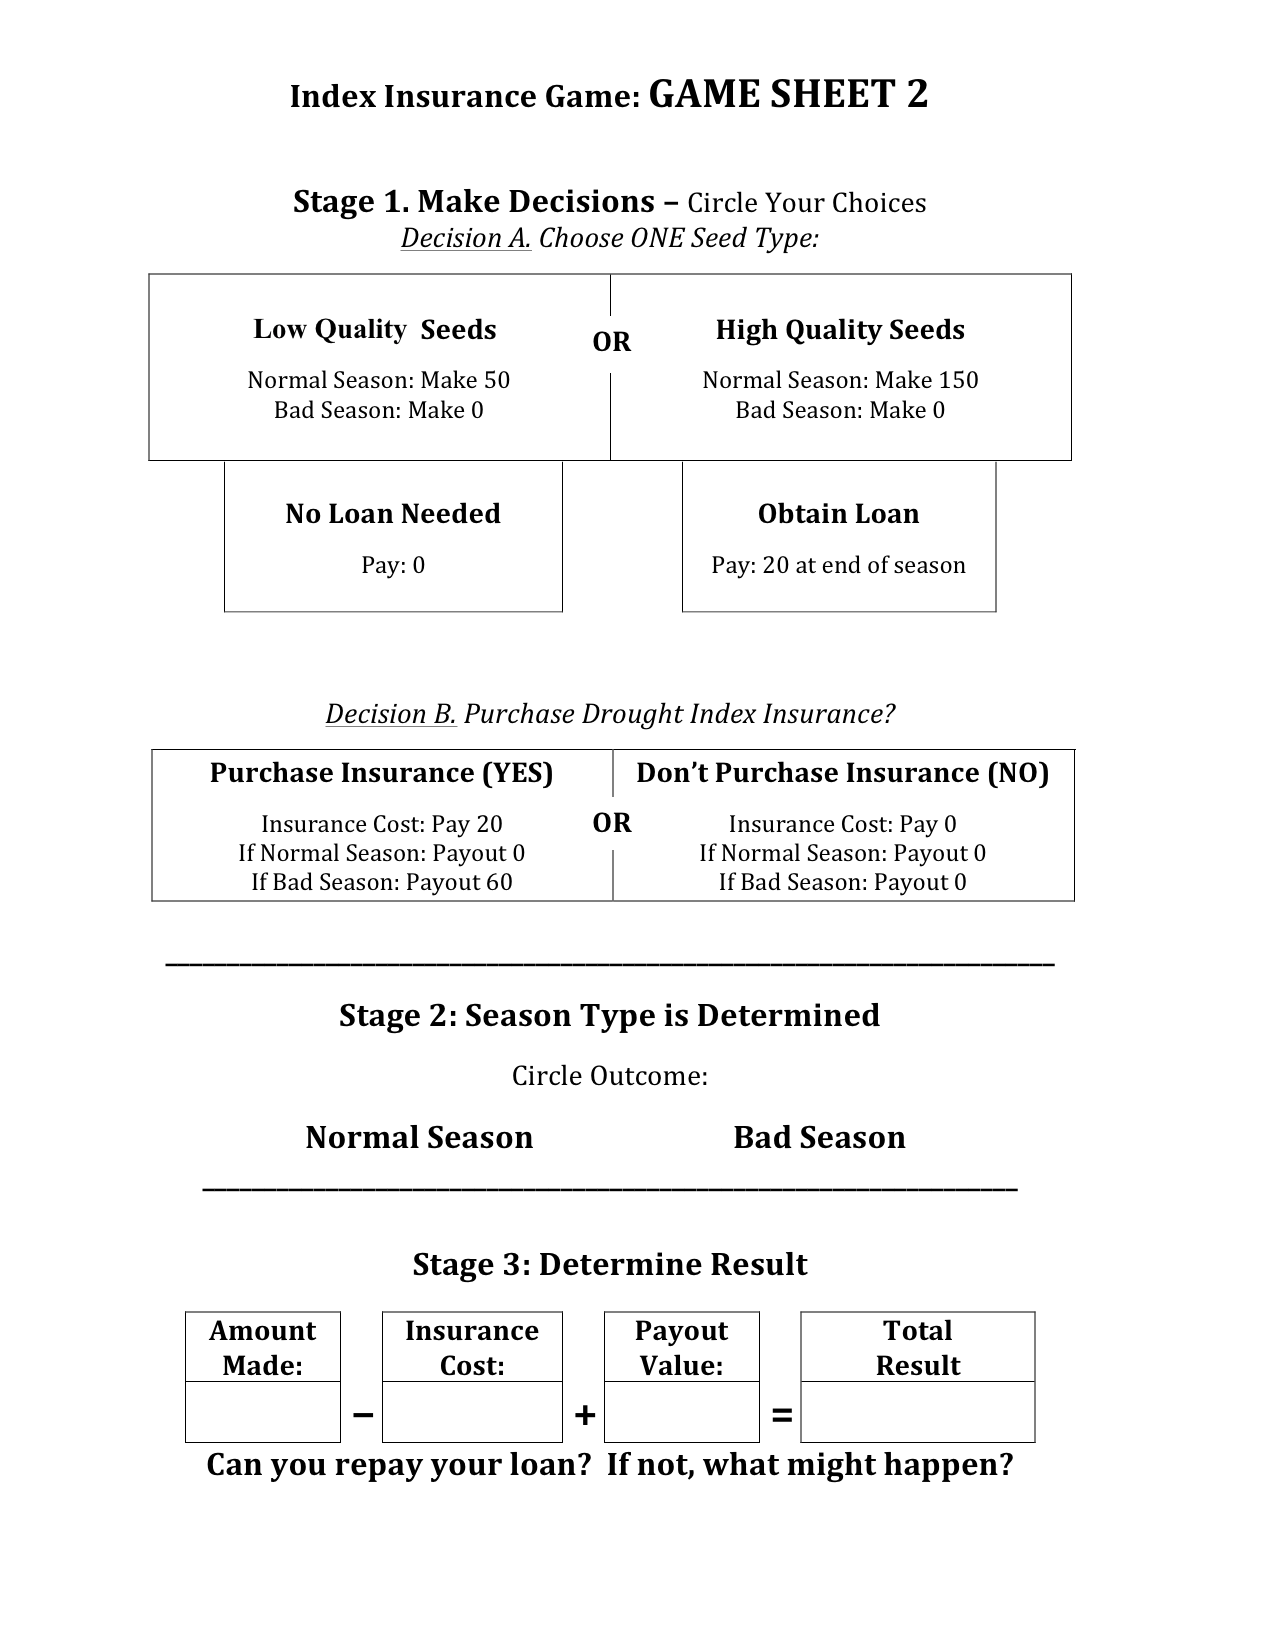
\includegraphics{indexinsurancegame2_en.png}}
\end{figure}

\textbf{Instructions}

This game sheet introduces insurance into the decision process. The concept of index insurance and when it pays out should be carefully explained.

\textbf{Discussion Questions}
\begin{enumerate}
\item {} 
What are the outcomes if there is a bad year? If there is a normal year?

\item {} 
What can a farmer do so that s/he’s less likely to have a bad outcome?

\item {} 
When would you buy insurance? Would you buy insurance with high quality or low quality seeds? When would you be glad to have bought insurance?

\end{enumerate}

\textbf{Key Points}
\begin{itemize}
\item {} 
Insurance can help make productive decisions less risky.

\end{itemize}


\subsection{Game Sheet 3}
\label{games/gameinstructions_quickreference_en:game-sheet-3}\begin{figure}[htbp]
\centering

\scalebox{0.330000}{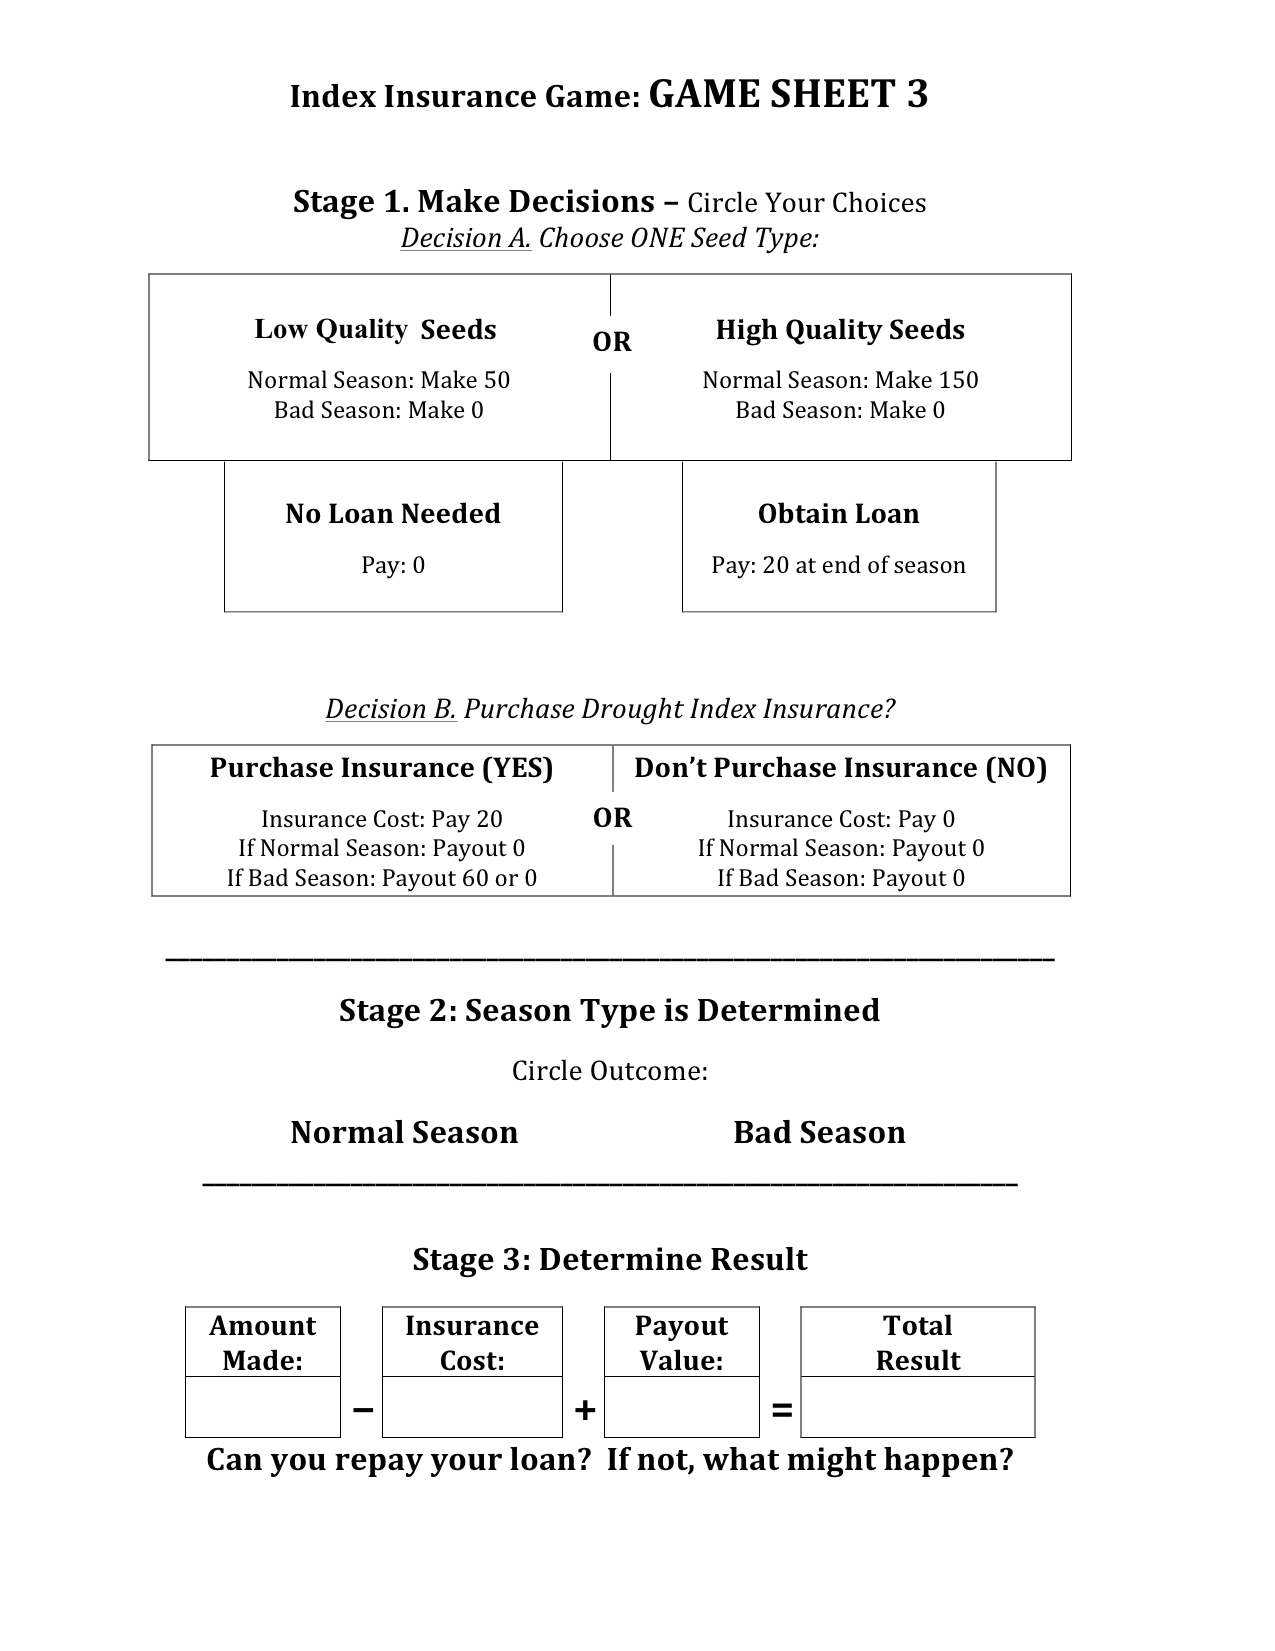
\includegraphics{indexinsurancegame3_en.png}}
\end{figure}

\textbf{Instructions}

With this game sheet discuss conditions under which the drought index insurance does not pay out: floods, pests, rainfall measurement mistakes, or the index could be focusing on the wrong time of the season. In order for the insurance to pay out the exact terms of the contract must be met. There are two key conditions:
\begin{enumerate}
\item {} 
it only pays out when a bad season is caused by drought; and

\item {} 
it only pays out when low level of rainfall is within the agreed upon contract dates

\end{enumerate}

If we were to consider a 15 year period, there should be 3 years that could be considered a drought period. Two of these years would get payouts, but one of these years would not. Therefore, there is a 1-in-5 chance of a bad year and a 1-in-3 chance that the insurance does not pay out in a bad year, there is technically only a 1-in-15 chance that a farmer will experience a bad year, which does not have a payout. In order to determine if it is a bad season with a payout, a die will be rolled. If the die lands on a 5 or a 6, there is \textbf{no payout}.

\textbf{Discussion Questions}
\begin{enumerate}
\item {} 
Have your decisions regarding the upcoming season changed now that the insurance does not pay every time? If yes, how?

\item {} 
What would have happened in a bad year without a payout? Are you worse off now than you were without insurance?

\item {} 
Is it enough to just purchase insurance in order to protect yourself from risk? How can you protect yourself during the years when index insurance fails to protect you? What other risk management strategies could you use?

\end{enumerate}

\textbf{Key Points}
\begin{itemize}
\item {} 
Index insurance cannot cover all the risk. There will be some bad seasons that do not merit a payout.

\end{itemize}


\subsection{Game Sheet 4}
\label{games/gameinstructions_quickreference_en:game-sheet-4}\begin{figure}[htbp]
\centering

\scalebox{0.330000}{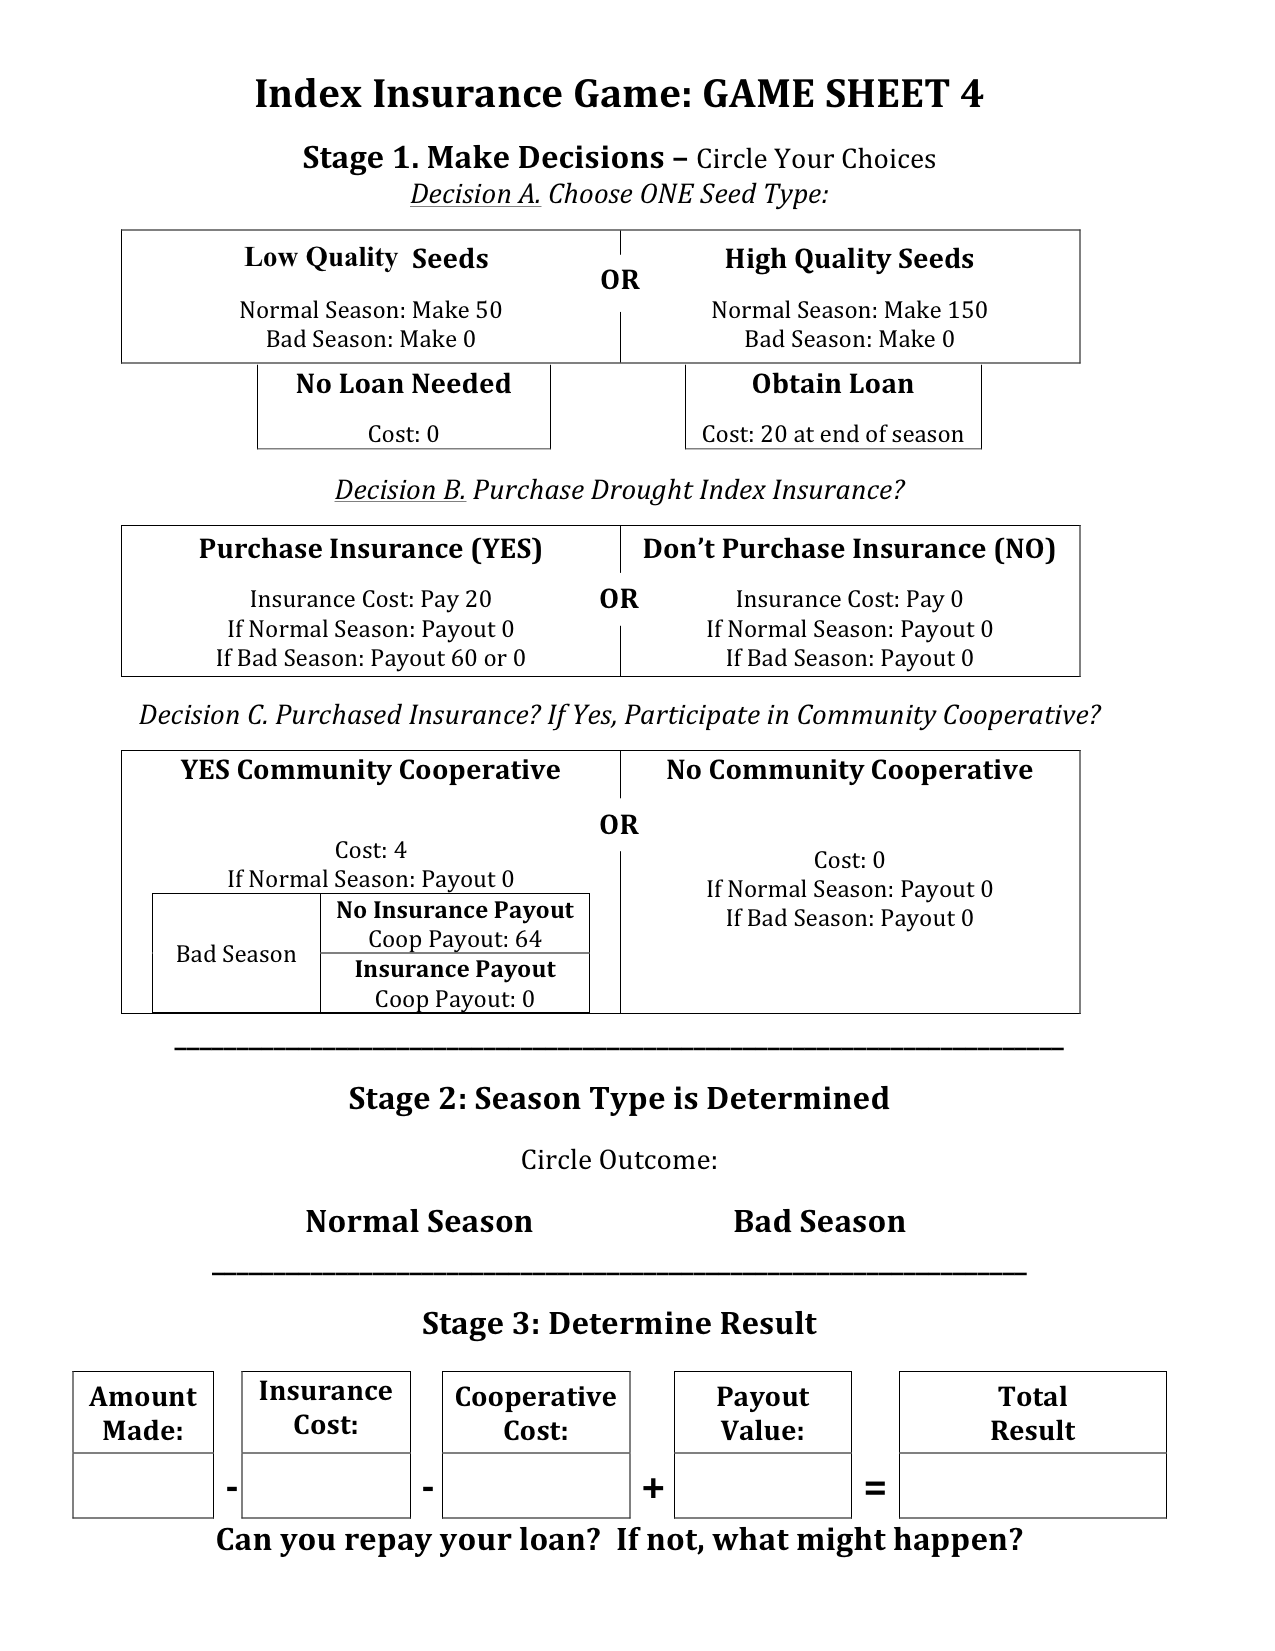
\includegraphics{indexinsurancegame4_en.png}}
\end{figure}

\textbf{Instructions}

This game sheet emphasizes the fact that index insurance is only a part of a risk management toolkit, and that there are other ways for farmers to manage risk. It introduces the idea of a community cooperative that would pay out in years when the insurance does not.

\textbf{Discussion Questions}
\begin{enumerate}
\item {} 
If you participate in the community cooperative would you still do well in a good year?

\item {} 
Would you like to participate in the cooperative if you know that insurance isn’t perfect and does not pay out every time?

\item {} 
What would happen this year if the season was bad and there wasn't a payout? How would the cooperative help during this year? Can you think of any other ways you can manage the insurance not paying out?

\end{enumerate}

\textbf{Key Points}
\begin{itemize}
\item {} 
Index insurance can be complimented by other risk management tools

\end{itemize}


\chapter{INDEX INSURANCE GAME: POSSIBLE GAME OUTCOMES}
\label{games/gameresults_en_Web:index-insurance-game-possible-game-outcomes}\label{games/gameresults_en_Web::doc}\begin{figure}[htbp]
\centering

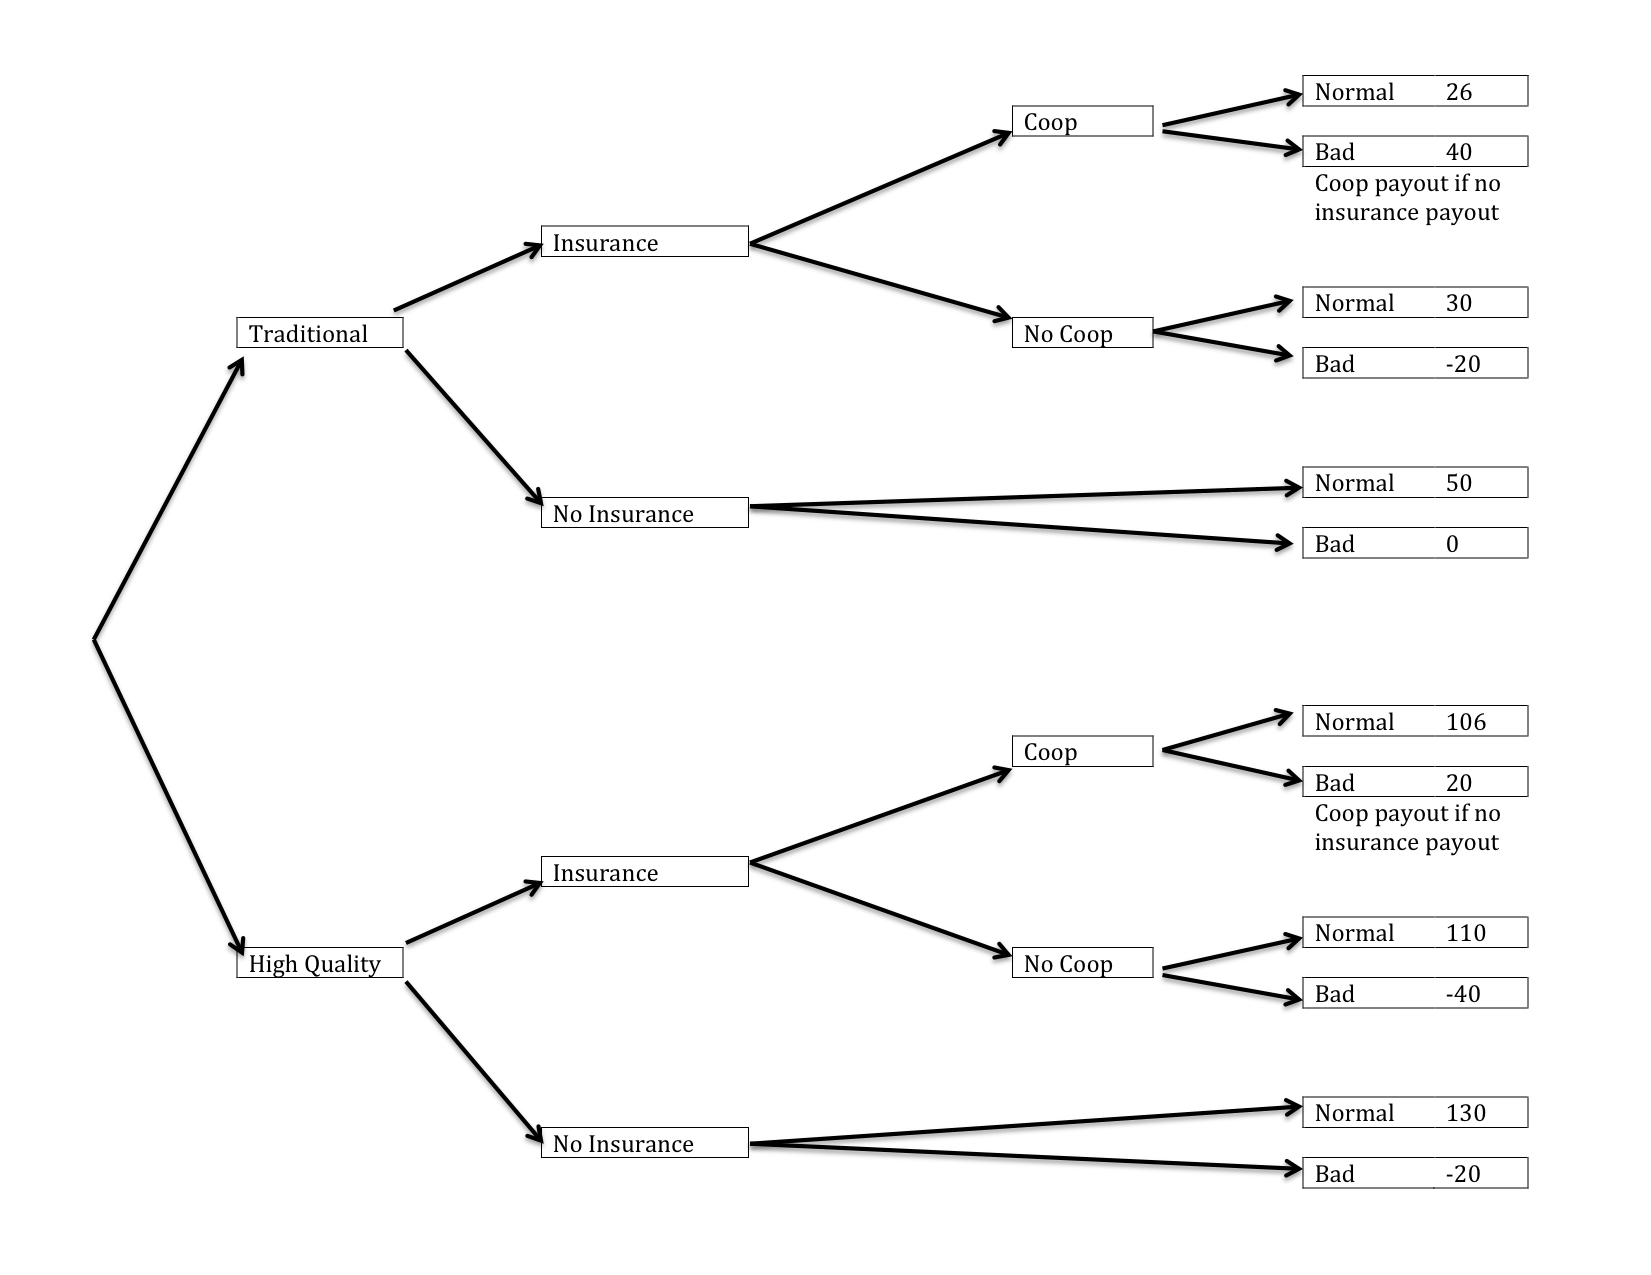
\includegraphics{gameresults.png}
\end{figure}


\chapter{WHAT IS WEATHER INDEX INSURANCE?}
\label{index_updated_educationalMat:what-is-weather-index-insurance}

\section{What is Weather Index Insurance?}
\label{whatisindexinsurance/weather/weatherindexinsurance_en::doc}\label{whatisindexinsurance/weather/weatherindexinsurance_en:what-is-weather-index-insurance}

\subsection{Topic: What is Weather Index Insurance?}
\label{whatisindexinsurance/weather/weatherindexinsurance_en:topic-what-is-weather-index-insurance}

\subsubsection{Objective}
\label{whatisindexinsurance/weather/weatherindexinsurance_en:objective}
The objective of this section is to introduce the reader to the concept of weather index insurance, how it differs from more traditional crop insurance products, and to describe how weather index insurance might fit within a farmer's overall risk management strategy/portfolio.


\subsubsection{Introduction: What is Insurance?}
\label{whatisindexinsurance/weather/weatherindexinsurance_en:introduction-what-is-insurance}
Insurance is a financial arrangement that is intended to provide protection from risk. This risk can be for any number of things, including death, a car accident, or even for crop losses. Insurance is not a gift or a subsidy, but a way in which a person can pay a small amount in good years and receive protection in bad years. However, you should expect that over time the amount that you pay will ALWAYS be more than the amount you receive to pay for the profit of the insurance company that holds your risk for you.

To obtain insurance, one must agree to and sign a contract with an insurance company. In exchange for a fixed, upfront payment called a ``premium'', the insurance company provides a guaranteed compensation if the specified contract terms (usually relating to a loss) occur. However, if something bad happens that is not covered by the contract, than the purchaser is not given money. In addition, if the agreed upon loss does not occur, you will not get your premium back. One benefit of purchasing insurance is that there are pre-agreed upon terms that dictate the amount of compensation you receive.


\subsubsection{Traditional Insurance verse Index Insurance?}
\label{whatisindexinsurance/weather/weatherindexinsurance_en:traditional-insurance-verse-index-insurance}
Index insurance is a relatively new tool that farmers can use to help manage risk. It pays out based on an index, such as rainfall, measured at a local weather station or by satellite, rather than based on a consequence of weather, such as a farmer's crop yield. This subtle distinction resolves a number of fundamental problems that makes traditional insurance unworkable in rural parts of developing countries. Unlike traditional crop insurance, the insurance company does not need to visit a farmer's field to determine premiums or assess damages; if the rainfall amount is below a pre-specified threshold, then the insurance pays out. Since the payout is not linked to the crop survival or failure, the farmer always has an incentive to make the best decisions for crop survival. This innovation significantly lowers the insurance company's transaction costs and risks, reducing insurance premiums and increasing accessibility.


\subsubsection{How Does Drought Index Insurance Work?}
\label{whatisindexinsurance/weather/weatherindexinsurance_en:how-does-drought-index-insurance-work}
Erratic rainfall is a problem for farmers. If the fields do not receive enough rainfall at the right times, then the crops will wither and die. Drought index insurance is a way to possibly protect against some of the losses associated with below average rainfall. If there is a drought (i.e. low rainfall over a given period of time), and this drought falls under the terms agreed to in the insurance contract, than the farmer will receive money to help make up for some of the loss.

Let's pretend you have a crop in the field, from which you will earn 10 dollars in a normal year. If there is a drought, indicated by a lack of rainfall, you may only earn 2 or 3 dollars instead, since much of the crop will likely be lost. If you had purchased insurance before the start of the season, and the rainfall during the drought was below the amount needed to trigger your insurance contract, then the insurance company will pay you some money.

It is important to note that the exact terms of the contract must be met for a payout.  If there is no drought, the insurance company will not pay anything, even if you have a bad year due to other factors like floods or pests. If there is bad rainfall during part of the year, but this low level of rainfall does not fall within the agreed upon contract dates, then the insurance company will not compensate the farmer.


\subsubsection{Index Insurance As the Last Piece}
\label{whatisindexinsurance/weather/weatherindexinsurance_en:index-insurance-as-the-last-piece}
We have found that insurance works best when it is combined with other development and disaster management strategies. Index insurance is not a stand-alone solution, but one tool of many. It works most effectively when it is addressing a clearly defined risk, such as drought, with other risks covered by other risk management options. It is almost always cheaper to reduce your risk (through irrigation or terracing or using improved seeds) than to transfer it by purchasing insurance. \textbf{Therefore, insurance works best when it addresses risks that cannot be reduced in other ways. For example, national cooperative movements, farmer credit access programs, contract farming and rural development programs all act as platforms for index insurance.} These programs help to manage a variety of risks for farmers, allowing index insurance to effectively target a very specific risk. Insurance should be built to address the risks remaining when these other interventions have been developed.


\subsubsection{Key Points}
\label{whatisindexinsurance/weather/weatherindexinsurance_en:key-points}\begin{enumerate}
\item {} 
For drought index insurance, payouts are determined by the amount of rainfall measured by rain gauges or satellites, not by the actual amount of rainfall that falls on your field.  This is a limitation of the insurance that you should think about when deciding if you want to purchase it.

\item {} 
You must pay for index insurance.  It is not a subsidy; you pay for what you get.

\item {} 
Index insurance cannot be used to address every risk; rather it is one part of a larger risk management package.

\item {} 
Farmers will still experience bad years in which their losses are not fully covered, or covered at all by their insurance contracts.

\item {} 
You will not receive a payment in most years, and you will not receive a payment in all bad years.

\item {} 
There are many things that drought index insurance is NOT designed to help with, like floods or termites. You will only be compensated when the specific contract terms are met.

\item {} 
If and when you receive an insurance payout it does not need to be paid back. It is the payment that is made to you in return for the premium that you bought as a climate risk management strategy.

\item {} 
Typically, a premium covers one year only and is not cumulative. You can make the decision each year as to whether or not you wish to purchase insurance; if yes, then you can pay the premium and receive coverage for that specific year. Your commitment is only for the one year.

\end{enumerate}


\subsection{Checkpoint: What is Weather Index Insurance?}
\label{whatisindexinsurance/weather/weatherindexinsurance_en:checkpoint-what-is-weather-index-insurance}
\emph{Note: Please answer ``True'' if you agree with the following statement, or ``False'' if you believe that the following statement is incorrect. When the group is finished, we will go over these statements together and correct the false sentences.}

\textbf{Questions}

\emph{Example:} By purchasing weather index insurance, any kind of damage to or loss of my crops will be covered. \textbf{False} \emph{By purchasing weather index insurance, only the terms agreed to in the contract will be covered.}
\begin{enumerate}
\item {} 
To obtain insurance, one must agree to and sign a contract with an insurance company. \_\_\_\_\_\_\_\_\_\_\_

\item {} 
If the terms of the insurance contract are fulfilled and the specific loss covered does occur, I will receive a pre-agreed upon payment. \_\_\_\_\_\_\_\_\_\_\_\_\_\_

\item {} 
If there is a bad rainfall year, but this low level of rainfall does not fall within the agreed upon contract dates, I will still receive a payout. \_\_\_\_\_\_\_\_\_\_\_\_\_\_

\item {} 
The exact terms of a contract must be met for a payout to occur. \_\_\_\_\_\_\_\_\_\_\_\_\_\_\_

\item {} 
Insurance can help cover all my risks and alone act as my disaster management tool. \_\_\_\_\_\_\_\_\_\_\_\_\_\_\_\_

\item {} 
With this type of index insurance, I will receive a payment in most years. \_\_\_\_\_\_\_\_\_\_\_\_

\item {} 
I will not receive a payment in all bad years. Farmers will still experience bad years that are not fully covered or covered at all by their insurance contracts. \_\_\_\_\_\_\_\_\_\_\_\_\_\_\_

\item {} 
Typically, insurance needs to be repurchased each year and only covers one year at a time. Your commitment is only for the one year. \_\_\_\_\_\_\_\_\_\_\_\_

\end{enumerate}


\section{Checkpoint Answer Key: What is Weather Index Insurance?}
\label{whatisindexinsurance/weather/weatherindexinsuranceanskey_en:checkpoint-answer-key-what-is-weather-index-insurance}\label{whatisindexinsurance/weather/weatherindexinsuranceanskey_en::doc}
\textbf{Answers}

\emph{Example:} By purchasing weather index insurance, any kind of damage to or loss of my crops will be covered. \textbf{False} \emph{By purchasing weather index insurance, only the terms agreed to in the contract will be covered.}
\begin{enumerate}
\item {} 
To obtain insurance, one must agree to and sign a contract with an insurance company. \textbf{True}

\item {} 
If the terms of the insurance contract are fulfilled and the specific loss covered does occur, I will receive a pre-agreed upon payment. \textbf{True}

\item {} 
If there is a bad rainfall year, but this low level of rainfall does not fall within the agreed upon contract dates, I will still receive a payout. \textbf{False} \emph{If there is a bad rainfall year, but this low level of rainfall does not fall within the agreed upon contract dates, I will NOT receive a payout.}

\item {} 
The exact terms of a contract must be met for a payout to occur. \textbf{True}

\item {} 
Insurance can help cover all of my risks and alone act as my disaster management tool. \textbf{False} \emph{Insurance cannot help cover all of my risks and works best when it is combined with other development and disaster management strategies. Index insurance is not a stand-alone solution, but one tool of many.}

\item {} 
With this type of index insurance, I will receive a payment in most years. \textbf{False} \emph{With this type of index insurance, I will not receive a payment in most years.}

\item {} 
I will not receive a payment in all bad years. Farmers will still experience bad years that are not fully covered, or covered at all by their insurance contracts. \textbf{True}

\item {} 
Typically, insurance needs to be repurchased each year and only covers one year at a time. Your commitment is only for the one year. \textbf{True}

\end{enumerate}


\section{Understanding a Drought Index}
\label{whatisindexinsurance/understandingadroughtindex_en_Web:understanding-a-drought-index}\label{whatisindexinsurance/understandingadroughtindex_en_Web::doc}

\subsection{Topic: Understanding a Drought Index}
\label{whatisindexinsurance/understandingadroughtindex_en_Web:topic-understanding-a-drought-index}

\subsubsection{Objective}
\label{whatisindexinsurance/understandingadroughtindex_en_Web:objective}
The objective of this section is to help the reader learn how to understand the particular aspects and features of a simple index insurance contract.  Topics covered include how index insurance payouts are determined using triggers and exits, contract features such as the contract ‘window’ and contract ‘phases’, and how and why to ‘cap’ your index measurements.  To make the analysis more concrete, we use adopt the specific example of a drought index insurance contract throughout this section.


\subsubsection{Introduction: Review of Index Insurance Contracts}
\label{whatisindexinsurance/understandingadroughtindex_en_Web:introduction-review-of-index-insurance-contracts}
Insurance contracts, in this case, are agreements between farmers and an insurance company. By signing an index insurance contract, the farmer agrees to pay a certain amount of money (called the premium) to enroll in the index insurance program. In return, if the contract is for drought insurance, then after the season (or contract window) is finished, if the rainfall is less than the amount agreed upon, the insurance company agrees to compensate the farmer. Participation in an insurance contract is voluntary and, typically, is only for one year; which is to say that the farmer must agree to the contract every year.


\subsubsection{Description of some important contract components:}
\label{whatisindexinsurance/understandingadroughtindex_en_Web:description-of-some-important-contract-components}
\textbf{Determining Payouts using Triggers and Exits:} During the dates covered by a drought index insurance contract (often these dates are called the ‘contract window’), the amount of rainfall measured by satellite or rain gauges determines if any payout is received. Each contract window has what is called a `trigger'; if the total rainfall amount is more than the trigger, there is no payment. Any rainfall total below the trigger will result in a payout. Payments will increase for each millimeter (mm) that rainfall falls further below the trigger, until a maximum payment is reached. The maximum payout point is called the index `exit'. To summarize, if the total rainfall for the contract dates is above the trigger, you will receive no payment. If the rainfall is between the trigger and exit, you will receive a partial payment. If the rainfall is below the exit, you will receive a full payment. The figure below illustrates how the payout is determined by the trigger and exit values:
\begin{figure}[htbp]
\centering

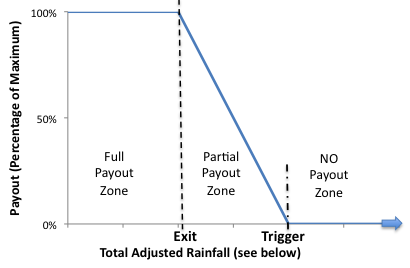
\includegraphics{chpt4ima1.png}
\end{figure}

\textbf{Contract Window:}  The contract window specifies the period of time during the cropping season to which the index insurance contract applies.  Typically, an index insurance contract will have both a start and an end date during which the index value is measured.  A drought insurance contract, for example, will only pay out if measured rainfall is below the index’s trigger value during the period specified by the contract window.  If rainfall is low outside of the dates specified by the window, the contract will not pay out.

\textbf{Measuring Rainfall: Using a Cap:} Please note that the rainfall total we use is actually an adjusted rainfall total. Every ten-day period (dekad) the rainfall amount is totaled, and a `cap' (e.g. 25 mm) is applied. This cap represents the maximum amount of rainfall that is counted for each ten-day period. These adjusted ten-day rainfall totals are then added together to calculate the adjusted rainfall total for the full contract window. A cap is applied so we can better capture dry spells. Without this feature, it would be possible to have a single big storm drop enough rainfall in a short amount of time to pass the contract trigger; however, you might still have very dry crops on all other days (while most of the water from the big storm would be washed away before it could be used by the plants). As a result of this adjustment, the contract triggers and exits are also not truly represented in units of millimeters. Instead, you may want to think of the trigger and exit as `capped millimeters'.

\textbf{Contract Phases:} In some locations, farmers have identified multiple critical periods in which their crops are vulnerable to drought. It is possible to develop an index that targets different phases (or windows) within the growing season. In a multiple phase contract, each phase can have a unique trigger, exit and payout frequency. However, not all crops and locations require a multiple phase insurance contract; a one-phase contract (only looking at one part of the season) is also possible.  Ultimately, the decision on which (and how many) phases to use will depend on local needs.

\textbf{Please Remember That:} Drought index insurance will not pay out in every year, and it will not cover all farmer risks. There are many things drought index insurance is NOT designed to help with, like floods or termites. You will not receive a payment in most years, and you will not receive a payment in all `bad' years. This insurance cannot be used to address every risk; rather it is designed to be one part of a larger risk management package.


\subsection{Checkpoint: Understanding a Drought Index}
\label{whatisindexinsurance/understandingadroughtindex_en_Web:checkpoint-understanding-a-drought-index}
\emph{Note: This is an example drought index insurance contract for a village, based on the R4 project in Ethiopia. The farmer design team has indicated that rainfall is very important in two parts of the planting season, so a two-phase contract was developed. Basically, these two phases can be treated as two separate contracts, since it is possible for the payment of insurance to be triggered in either part of the season. For the questions below, we will only be examining the first phase of the contract (i.e. we will only look at the first and second columns of the table).}


\begin{threeparttable}
\capstart\caption{Contract Example: Adi Ha, Ethiopia (Maize)}

\begin{tabulary}{\linewidth}{|L|L|L|}
\hline
\textsf{\relax 
Title
} & \textsf{\relax 
Phase 1
} & \textsf{\relax 
Phase 2
}\\
\hline
Start Period: (Dekad*)
 & 
May-1 (13)
 & 
21-Aug (24)
\\
\hline
End Period: (Dekad*)
 & 
30-June (18)
 & 
20-Sep (26)
\\
\hline
Trigger (mm)
 & 
13
 & 
30
\\
\hline
Exit (mm)
 & 
7
 & 
20
\\
\hline
Cap  (mm/dekad*)
 & 
25
 & 
25
\\
\hline\end{tabulary}

\end{threeparttable}



\begin{threeparttable}
\capstart\caption{Payout Example: Adi Ha, Ethiopia (Maize)}

\begin{tabulary}{\linewidth}{|L|L|L|}
\hline
\textsf{\relax 
Historic Years
} & \textsf{\relax 
Phase 1: Percent of Max Payout Received (\%)
} & \textsf{\relax 
Phase 2: Percent of Max Payout Received (\%)
}\\
\hline
1995
 & 
0
 & 
0
\\
\hline
1996
 & 
0
 & 
0
\\
\hline
1997
 & 
0
 & 
51
\\
\hline
1998
 & 
0
 & 
0
\\
\hline
1999
 & 
0
 & 
0
\\
\hline
2000
 & 
97
 & 
0
\\
\hline
2001
 & 
0
 & 
0
\\
\hline
2002
 & 
0
 & 
0
\\
\hline
2003
 & 
0
 & 
0
\\
\hline
2004
 & 
8
 & 
0
\\
\hline
2005
 & 
0
 & 
0
\\
\hline
2006
 & 
0
 & 
0
\\
\hline
2007
 & 
0
 & 
0
\\
\hline
2008
 & 
0
 & 
0
\\
\hline
2009
 & 
74
 & 
0
\\
\hline\end{tabulary}

\end{threeparttable}

\begin{itemize}
\item {} 
a dekad is a period of ten days

\end{itemize}

\textbf{Questions: (Using the first phase of the contract only)}
\begin{enumerate}
\item {} 
What is the start date of the phase 1 contract? \_\_\_\_\_\_\_\_\_\_\_\_\_\_\_\_\_\_

\item {} 
For the start date, what does the number in parentheses represent? \_\_\_\_\_\_\_\_\_\_\_\_\_\_\_

\item {} 
What is the end date of the phase 1 contract? \_\_\_\_\_\_\_\_\_\_\_\_\_\_\_\_\_\_\_\_\_\_\_\_\_\_\_\_\_\_\_\_\_\_\_\_

\item {} 
What is the trigger of the phase 1 contract (mm)?  What does this mean? \_\_\_\_\_\_\_\_\_\_\_

\item {} 
What is the exit of the phase 1 contract (mm)?  What does this mean? \_\_\_\_\_\_\_\_\_\_\_\_\_\_

\item {} 
If the total rainfall during the contract window is 10mm, will there be a payout? If Yes, would this be a partial or full payout? \_\_\_\_\_\_\_\_\_\_\_\_\_\_\_\_\_\_\_\_\_\_

\item {} 
What is the maximum amount of rainfall that is counted for each dekad? \_\_\_\_\_\_\_\_\_\_\_\_

\item {} 
According to this example contract, how many phase 1 payouts would there have been in the last 15 years? \_\_\_\_\_\_\_\_\_\_\_\_\_\_\_

\item {} 
What years would have paid out for the 1st phase? \_\_\_\_\_\_\_\_\_\_\_\_\_\_\_\_\_\_\_\_\_

\item {} 
Which year would have paid out the most?  What percentage of a maximum payout? Why does the percent of maximum payout received change for different years? \_\_\_\_\_\_\_\_\_\_\_\_\_\_\_

\end{enumerate}


\section{Checkpoint Answer Key: Understanding a Drought Index}
\label{whatisindexinsurance/understandingadroughtindexanskey_en::doc}\label{whatisindexinsurance/understandingadroughtindexanskey_en:checkpoint-answer-key-understanding-a-drought-index}
\textbf{Answers}
\begin{enumerate}
\item {} 
What is the start date of the phase 1 contract? \textbf{1-May}

\item {} 
For the start date, what does the number in parentheses represent? \textbf{The dekad or 10-day period in of the year in which the contract will begin}

\item {} 
What is the end date of the phase 1 contract? \textbf{30-June}

\item {} 
What is the trigger of the phase 1 contract (mm)? What does this mean? \textbf{13mm:} \emph{This means that there will only be a payout if rainfall is less than 13mm}

\item {} 
What is the exit of the phase 1 contract (mm)? What does this mean? \textbf{7mm:} \emph{This means that if there is less than 7mm of rainfall, there will be a full payout.}

\item {} 
If the total rainfall during the contract window is 10mm, will there be a payout? If Yes, would this be a partial or full payout? \textbf{Yes (partial payout)}

\item {} 
What is the maximum amount of rainfall that is counted for each dekad? \textbf{25mm}

\item {} 
According to this example contract, how many phase 1 payouts would there have been in the last 15 years? \textbf{3}

\item {} 
What years would have paid out for the 1st phase? \textbf{2000, 2004, 2009}

\item {} 
Which year would have paid out the most?  What percentage of maximum payout? Why does the percent of maximum payout received change for different years? \textbf{2000, 97\%:} \emph{The percent of maximum payout received changes for different years because the rainfall would have been at different levels between the trigger and the exit.}

\end{enumerate}


\chapter{GATHERING INFORMATION TO BEGIN THE DESIGN PROCESS}
\label{index_updated_educationalMat:gathering-information-to-begin-the-design-process}

\section{Initial Visit Interaction to Determine the Worst Years}
\label{games/initialvisitexercise_Ethiopia::doc}\label{games/initialvisitexercise_Ethiopia:initial-visit-interaction-to-determine-the-worst-years}

\subsection{Background/Objectives}
\label{games/initialvisitexercise_Ethiopia:background-objectives}
In this section of the initial visit, farmers will identify the worst years and they will discuss the reasons why the years were the worst. During this exercise, farmers will name the worst 8 years (that they can remember) in the past 31 years for their main crop. This exercise will be used in conjunction with the initial visit materials, where index insurance concepts are introduced through educational games and discussions with the design team.


\subsection{Instructions for facilitators}
\label{games/initialvisitexercise_Ethiopia:instructions-for-facilitators}

\subsubsection{Preliminary preparation}
\label{games/initialvisitexercise_Ethiopia:preliminary-preparation}
List of suggested supplies
\begin{itemize}
\item {} 
Chalkboard/dry erase board/ flip chart

\item {} 
Markers/chalk to write on the board

\item {} 
Several different types/colors of post-its

\item {} 
Paper and pen for the facilitators to record the results of the exercise

\item {} 
Facilitators instructions and Worst Year Questions

\end{itemize}

Note: if the facilitators cannot use the suggested supplies in the field, some of these items can be replaced by more basic objects. As an example, the years might be represented by 15 boxes placed on the ground and the post-its can be replaced by beans or leaves of different colors. If facilitators find particularly effective tools, please let us know so that we can mention them in the materials.

Before starting, the facilitator draws a table on the whiteboard/chalkboard as follows:
\begin{figure}[htbp]
\centering

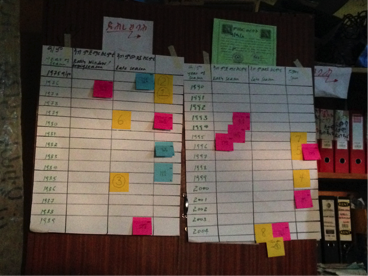
\includegraphics{postitsInteractiveExercise.png}
\end{figure}

\emph{Farmers' Worst Years Chart}

Facilitator should go over the game instructions as set out below.


\subsubsection{Exercise instructions}
\label{games/initialvisitexercise_Ethiopia:exercise-instructions}
\emph{Note: As long as you collect all the information required (questions listed below), you can modify the exercises depending on the community, and your knowledge of local cropping practices. For example, in some communities you might have a lot of previous knowledge and the exercise will take less time. In communities, where you really need to collect information on worst years, timing and impacts, you will need to spend more time going through the exercise.}
\begin{enumerate}
\item {} 
Assign participants in groups of 4-5 people (keep the same groups from the index insurance educational game). At least one person in each group should be able to read/write (can be a farmer or an assistant). Provide each group with several post-its of the same color (or other objects suitable to use in the field). Each group should have 3-6 post-its.

\item {} 
Ask each group to select a representative who would be responsible to place the post-its in the appropriate place on the board once the group reaches consensus on the worst 3 years.

\item {} 
Discuss with the farmers and agree together on a crop (or several crops) that they would like to use the insurance for. Some crops might not be suitable for an index insurance product (e.g. vegetables). In the interactive exercise ask farmers to identify years that were bad for the selected crops. Ask the participants to identify which years were bad in the early and late season.

\item {} 
Explain to each group that this is an interactive exercise where participants in each group must discuss which years were the worst, based on their experience and memory. Ask each group to discuss and identify the 8 worst years. The eight worst years will be represented by the post-its each group receives (or other objects that groups receive). The groups should rank the worst years (with the worst year being 1). Remember to designate the elected group representative to lead the discussion.

\item {} 
Give the groups 30 minutes to decide on the worst 8 years.

\item {} 
Now, ask the group representative to walk to the chart and place the post-its next to the worst years decided by his/her group.

\item {} 
After all groups have placed all their post-its on the \emph{Farmers’ Worst Years Chart}, compare the years reported by the different groups. If there are differences, give the participants a chance to discuss in one big group until they reach agreement on 8 common worst years in the last 30 years for their village.

\item {} 
Groups will also have to specify if the rainfall was particularly low at the start or at the end of the season. The facilitator can give an example like: ``If you had the worst year for your main crop because of a drought, was the precipitation lower than usual in the early or the late part of the rainy season?''

\item {} 
From all the years that the farmers listed, select the years for which there was strong disagreement between the farmer groups, and discuss the effects of the worst years until consensus is reached.

\item {} 
Make sure to take pictures of the worst years chart. Take notes on farmers’ feedback.

\end{enumerate}


\subsection{Worst Year Questions}
\label{games/initialvisitexercise_Ethiopia:worst-year-questions}\begin{enumerate}
\item {} 
What are the primary crops cultivated in the community? List below with estimated growing season for each.

\item {} 
What were the worst 8 years (for your main crop) that you can remember? List them in order starting with the worst one.

\item {} 
What caused the worst 8 years that you can remember (i.e. drought, hurricane etc.)?
\begin{enumerate}
\item {} 
List the causes for each of the eight years

\item {} 
In which phase of crop development did the events occur (i.e. flowering, planting etc.)?

\item {} 
During which month of the year did they occur (i.e. January etc.)?

\end{enumerate}

\item {} 
How frequently do bad years tend to occur (e.g. every 4 yrs)? Is there any pattern in the occurrence of these events?

\item {} 
In the years listed above, did you have access to climate information that helped you take action (e.g. traditional forecast methods, met service/weather report, recent trend of more frequent droughts)?

\end{enumerate}


\subsection{Effects of the Worst Year Questions}
\label{games/initialvisitexercise_Ethiopia:effects-of-the-worst-year-questions}\begin{enumerate}
\item {} 
How did it affect the farmers? List the different effects.

\item {} 
How did it affect the community (ex. migration in search of work)? List the different effects.

\item {} 
Who did it impact the most (what types of families, which local areas, etc.)?

\item {} 
How did it affect families? Did it affect women differently than men? How did it affect the role of women in the family?

\item {} 
During the worst year that you can remember, what actions did you undertake ahead of time to reduce the impact of climate events?

\item {} 
Did the government help you in the worst year? Did anyone else help you in the worst year? Who?

\end{enumerate}


\chapter{DESIGNING AN INDEX}
\label{index_updated_educationalMat:designing-an-index}

\section{Concepts Behind Index Design}
\label{whatisindexinsurance/conceptsbehindindexdesign_en_Web:concepts-behind-index-design}\label{whatisindexinsurance/conceptsbehindindexdesign_en_Web::doc}

\subsection{Topic: Setting Triggers and Exits}
\label{whatisindexinsurance/conceptsbehindindexdesign_en_Web:topic-setting-triggers-and-exits}

\subsubsection{Introduction}
\label{whatisindexinsurance/conceptsbehindindexdesign_en_Web:introduction}
The first two columns of the chart below show the amount of rainfall received during the end of the rainy season for 15 historic years. The second two columns begin to order the years by the amount of rainfall received, but have only been partially filled in. Using the information in this table, we will explore one way to set triggers and exits for an initial draft drought index that targets early cessation of the rainy season. This example is based on the R4 project, in Ethiopia.

The method used below is called historical burn analysis, as it relies on the past to provide a key to what might occur in the future. Using this approach, it is assumed that the coming year will look like one of the years that has already occurred. Therefore, the historical years are used to determine an appropriate trigger and exit for next season's index insurance contract. While this is a simplistic approach, it provides a starting point from which contracts can be further developed and refined.


\begin{threeparttable}
\capstart\caption{Setting Triggers and Exits Using Historical Burn Analysis}

\begin{tabulary}{\linewidth}{|L|L|L|L|L|}
\hline
\textsf{\relax 
Historical Year Rainfall (1995 - 2009)
} & \textsf{\relax } & \textsf{\relax } & \textsf{\relax 
Ordering Years by Rainfall Total
} & \textsf{\relax }\\
\hline
Year
 & 
Index Window Adjusted Rainfall Total (mm)*
 &  & 
Year
 & 
Index Window Adjusted Rainfall Total (mm)*
\\
\hline
1995
 & 
54.85
 &  & 
2003
 & 
79.31
\\
\hline
1996
 & 
74.42
 &  & 
1998
 & 
75.07
\\
\hline
1997
 & 
26.57
 &  & 
1996
 & 
74.42
\\
\hline
1998
 & 
75.07
 &  & 
2005
 & 
66.26
\\
\hline
1999
 & 
60.54
 &  & 
2001
 & 
62.6
\\
\hline
2000
 & 
54.76
 &  & 
1999
 & 
60.54
\\
\hline
2001
 & 
62.6
 &  & 
2006
 & 
58.64
\\
\hline
2002
 & 
51.81
 &  & 
2008
 & 
57.49
\\
\hline
2003
 & 
79.31
 &  & 
1995
 & 
54.85
\\
\hline
2004
 & 
31.84
 &  & 
2000
 & 
54.76
\\
\hline
2005
 & 
66.26
 &  &  & \\
\hline
2006
 & 
58.64
 &  &  & \\
\hline
2007
 & 
53.36
 &  &  & \\
\hline
2008
 & 
57.49
 &  &  & \\
\hline
2009
 & 
49.68
 &  &  & \\
\hline\end{tabulary}

\end{threeparttable}



\subsection{Checkpoint: Setting Triggers and Exits}
\label{whatisindexinsurance/conceptsbehindindexdesign_en_Web:checkpoint-setting-triggers-and-exits}
\emph{Note: Please use the following instructions to fill in the remaining spaces of the last two columns of the chart:}
\begin{enumerate}
\item {} 
First, order the above years and corresponding rainfall totals by the amount of rainfall received. Start with the largest rainfall total at the top of the chart and end with the least amount of rainfall at the bottom. The first ten rows have already been filled in to expedite this task. Please fill in the remaining blanks.

\item {} 
Draw a line separating the worst rainfall year from the years above. This line represents the Exit, or the point below which a complete payout is provided. In this initial draft index the Exit is designed so there is a full payout for the worst year in the past fifteen. Here, the Exit would be set to equal the worst year's rainfall total rounded up to the nearest whole number.

\item {} 
What is the Exit value for this contract? \_\_\_\_\_\_\_\_\_\_\_\_\_\_\_\_\_\_\_\_\_\_\_\_

\item {} 
Assume we are interested in a contract that would payout four times in the past fifteen years.  Draw a dotted line separating the worst four rainfall years from the years above. This line represents the Trigger for a contract that would payout four times in the past fifteen years. The first three years below this line would have resulted in partial payouts, while the worst year would have resulted in a full payout. For this initial draft index, the Trigger would be approximately halfway between the fourth and fifth worst years.

\item {} 
Choose a value to Trigger the contract: \_\_\_\_\_\_\_\_\_\_\_\_\_\_\_\_\_\_\_\_\_\_\_\_\_\_\_\_

\end{enumerate}


\section{Checkpoint: Designing an Initial Weather Index By Hand}
\label{whatisindexinsurance/designingindexbyhand::doc}\label{whatisindexinsurance/designingindexbyhand:checkpoint-designing-an-initial-weather-index-by-hand}

\subsection{Topic: Designing an Initial Weather Index By Hand}
\label{whatisindexinsurance/designingindexbyhand:topic-designing-an-initial-weather-index-by-hand}

\subsubsection{Overview}
\label{whatisindexinsurance/designingindexbyhand:overview}
IRI has developed software to aid in the creation and pricing of indices. In this exercise, you will mimic the process that the software uses by doing an index design of your own completely by hand, to gain insight into the index design process.

During this exercise, you will be receiving bits of new information in each :index:'Task' as you progress through your index design. Your job in this exercise is very similar to how it would be in the real world - you are sometimes forced to make decisions with limited information and do the best job you can with what you have at that moment. However, by the end of this exercise, you will be able to develop an initial index. Other educational material will discuss how to strengthen and validate the index.

This activity consist of 6 main tasks:
\begin{enumerate}
\item {} 
Gathering information about the village

\item {} 
Proposing an index window

\item {} 
Summing up historical rainfall estimates

\item {} 
Calculating triggers and exits

\item {} 
Calculating payouts

\item {} 
How to begin pricing your index

\end{enumerate}


\subsubsection{Context:}
\label{whatisindexinsurance/designingindexbyhand:context}
This exercise is based on an example from the 2011 HARITA project in Tigray, Ethiopia.
For the remainder of this exercise consider yourself as part of the HARITA project development team for 2011. Before an index is developed for a community, discussions should be held with farmers, community leaders and local experts to discuss relevant risk management strategies and cropping systems. For the sake of this exercise, it has already been determined that drought index insurance could be valuable to the farmers in the village and the community has requested that an index be designed to meet their needs. Your task is to design an index from start to finish. Good luck!


\subsubsection{Task 1: Gathering information about the village: Village X}
\label{whatisindexinsurance/designingindexbyhand:task-1-gathering-information-about-the-village-village-x}
Community and expert feedback is important for developing an index. This includes key planting and flowering dates, as well as past drought years. Sometimes all the information you gather will not perfectly agree, but a general consensus should be reached. If applicable, it can also be valuable to reference other indices that have been developed for nearby villages, if the villages have similar agroclimatology and planting strategies.

Below, we have assembled consensus information from the community of Village X and local experts, while also taking into account the index of a neighboring similar village:

{\hfill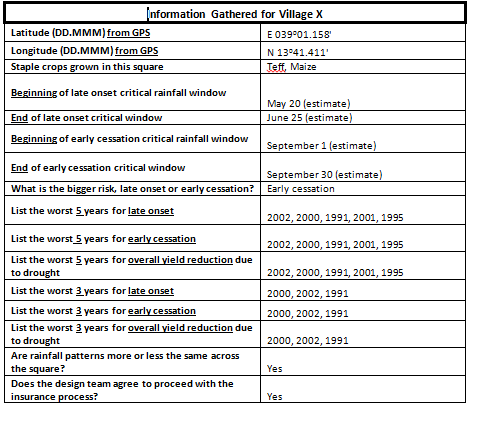
\includegraphics{villagex.png}\hfill}

\emph{Your Task: Answer these questions before proceeding to the next step.}
\begin{enumerate}
\item {} 
What are the most important crops grown in Village X? \_\_\_\_\_\_\_\_\_\_\_\_\_\_\_

\item {} 
What is the preferred starting date of the critical window for the planting (late onset) stage? \_\_\_\_\_\_\_\_\_\_\_\_\_\_\_

\item {} 
What is the preferred ending date of the critical window for the planting (late onset) stage? \_\_\_\_\_\_\_\_\_\_\_\_\_\_\_

\item {} 
What is the preferred starting date of the critical window for the flowering (early cessation) stage? \_\_\_\_\_\_\_\_\_\_\_\_\_\_\_

\item {} 
What is the preferred ending date of the critical window for the flowering (early cessation) stage? \_\_\_\_\_\_\_\_\_\_\_\_\_\_\_

\item {} 
What is the biggest agricultural risk that Village X faces? \_\_\_\_\_\_\_\_\_\_\_\_\_\_\_

\item {} 
During which of the two windows would you rather have insurance coverage to best address this risk? Late onset (planting) or early cessation (flowering)? \_\_\_\_\_\_\_\_\_\_\_\_\_\_\_

\end{enumerate}


\subsubsection{Task 2: Proposing an index window}
\label{whatisindexinsurance/designingindexbyhand:task-2-proposing-an-index-window}
Using the information provided in Task 1, it is now time to begin developing an index for Village X. In this task you will decide on appropriate index windows (start and end dates) for both the planting and flowering phases of the season; these two phase are intended to target the periods in which farmers identified their crops as being most vulnerable to drought. Be sure to come to a consensus in your group, and make use of the dekad conversion table on the next page.

\emph{Hint: The dates provided in the table in Task 1, may not always align perfectly with the start/end dates of a dekad. You may need to approximate in some cases.}

\emph{Your Task: Decide on the below factors for your new index.}
\begin{enumerate}
\item {} 
Proposed start dekad for the planting window: \_\_\_\_\_\_\_\_\_\_\_\_\_\_\_\_\_\_\_\_\_\_\_\_\_\_\_\_\_\_\_\_\_\_\_\_\_\_

\item {} 
Proposed end dekad for the planting window: \_\_\_\_\_\_\_\_\_\_\_\_\_\_\_\_\_\_\_\_\_\_\_\_\_\_\_\_\_\_\_\_\_\_\_\_\_\_\_

\item {} 
Proposed start dekad for the flowering window: \_\_\_\_\_\_\_\_\_\_\_\_\_\_\_\_\_\_\_\_\_\_\_\_\_\_\_\_\_\_\_\_\_\_\_\_\_

\item {} 
Proposed end dekad for the flowering window: \_\_\_\_\_\_\_\_\_\_\_\_\_\_\_\_\_\_\_\_\_\_\_\_\_\_\_\_\_\_\_\_\_\_\_\_\_\_

\end{enumerate}

Now you have set the windows for both indices, but you still have to determine appropriate trigger and exit values for each index. Step 3 and 4 will help you do this.

\begin{longtable}{|l|l|l|}
\hline
\textsf{\relax 
Start Day
} & \textsf{\relax 
Dekad
} & \textsf{\relax 
End Day
}\\
\hline\endfirsthead

\multicolumn{3}{c}%
{{\textsf{\tablename\ \thetable{} -- continued from previous page}}} \\
\hline
\textsf{\relax 
Start Day
} & \textsf{\relax 
Dekad
} & \textsf{\relax 
End Day
}\\
\hline\endhead

\hline \multicolumn{3}{|r|}{{\textsf{Continued on next page}}} \\ \hline
\endfoot

\endlastfoot


1-Jan
 & 
1
 & 
10-Jan
\\
\hline
11-Jan
 & 
2
 & 
20-Jan
\\
\hline
21-Jan
 & 
3
 & 
31-Jan
\\
\hline
1-Feb
 & 
4
 & 
10-Feb
\\
\hline
11-Feb
 & 
5
 & 
20-Feb
\\
\hline
21-Feb
 & 
6
 & 
28-Feb
\\
\hline
1-Mar
 & 
7
 & 
10-Mar
\\
\hline
11-Mar
 & 
8
 & 
20-Mar
\\
\hline
21-Mar
 & 
9
 & 
31-Mar
\\
\hline
1-Apr
 & 
10
 & 
10-Apr
\\
\hline
11-Apr
 & 
11
 & 
20-Apr
\\
\hline
21-Apr
 & 
12
 & 
30-Apr
\\
\hline
1-May
 & 
13
 & 
10-May
\\
\hline
11-May
 & 
14
 & 
20-May
\\
\hline
21-May
 & 
15
 & 
31-May
\\
\hline
1-Jun
 & 
16
 & 
10-Jun
\\
\hline
11-Jun
 & 
17
 & 
20-Jun
\\
\hline
21-Jun
 & 
18
 & 
30-Jun
\\
\hline
1-Jul
 & 
19
 & 
10-Jul
\\
\hline
11-Jul
 & 
20
 & 
20-Jul
\\
\hline
21-Jul
 & 
21
 & 
31-Jul
\\
\hline
1-Aug
 & 
22
 & 
10-Aug
\\
\hline
11-Aug
 & 
23
 & 
20-Aug
\\
\hline
21-Aug
 & 
24
 & 
31-Aug
\\
\hline
1-Sep
 & 
25
 & 
10-Sep
\\
\hline
11-Sep
 & 
26
 & 
20-Sep
\\
\hline
21-Sep
 & 
27
 & 
30-Sep
\\
\hline
1-Oct
 & 
28
 & 
10-Oct
\\
\hline
11-Oct
 & 
29
 & 
20-Oct
\\
\hline
21-Oct
 & 
30
 & 
31-Oct
\\
\hline
1-Nov
 & 
31
 & 
10-Nov
\\
\hline
11-Nov
 & 
32
 & 
20-Nov
\\
\hline
21-Nov
 & 
33
 & 
30-Nov
\\
\hline
1-Dec
 & 
34
 & 
10-Dec
\\
\hline
11-Dec
 & 
35
 & 
20-Dec
\\
\hline
21-Dec
 & 
36
 & 
31-Dec
\\
\hline\end{longtable}



\subsubsection{Task 3: Summing up historical rainfall estimates: Village X}
\label{whatisindexinsurance/designingindexbyhand:task-3-summing-up-historical-rainfall-estimates-village-x}
Drought indices can be triggered using rainfall data collected by rain gauges or satellites. There are advantages and disadvantages to both types of product and such decisions should be made on a project-by-project basis. In this example, decadal satellite rainfall estimates for the 10km by 10km square covering Village X are provided (on the next page). The satellite used to gather these measurements takes readings across all of Ethiopia, everyday. A cap of 25 millimeters has already been applied to this dekadal rainfall information. In other words, the maximum amount of rainfall that should be recorded for any dekad is 25mm

The start and end dates presented below might be in a format you have never seen before. For example the first start date is `1-Jan/23-Dec'. You should only look at the first date given (1-Jan), as this corresponds to the Gregorian (or Roman) calendar. The other date (23-Dec) is based on the local calendar in this example and should be ignored for this exercise.

\emph{Your Task: For the planting and flowering windows you selected in Step 2, add up the rainfall for every year since 1995. The table below will help you to do this. Then, in the third column, total the rainfall from the two phases (planting and flowering). Only use the first date listed in each box.}


\begin{threeparttable}
\capstart\caption{Fill In Table}

\begin{tabulary}{\linewidth}{|L|L|L|}
\hline
\textsf{\relax 
Year
} & \textsf{\relax 
Planting
} & \textsf{\relax 
Flowering
}\\
\hline
1995
 &  & \\
\hline
1996
 &  & \\
\hline
1997
 &  & \\
\hline
1998
 &  & \\
\hline
1999
 &  & \\
\hline
2000
 &  & \\
\hline
2001
 &  & \\
\hline
2002
 &  & \\
\hline
2003
 &  & \\
\hline
2004
 &  & \\
\hline
2005
 &  & \\
\hline
2006
 &  & \\
\hline
2007
 &  & \\
\hline
2008
 &  & \\
\hline
2009
 &  & \\
\hline
2010
 &  & \\
\hline\end{tabulary}

\end{threeparttable}


{\hfill\scalebox{0.700000}{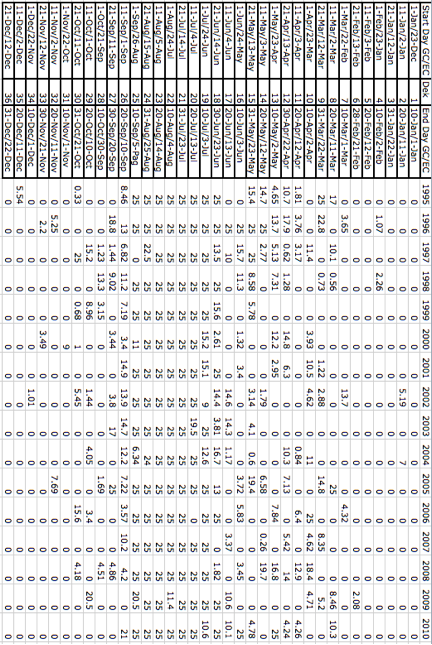
\includegraphics{summingrainfall.png}}\hfill}


\subsubsection{Task 4: Calculating triggers and exits}
\label{whatisindexinsurance/designingindexbyhand:task-4-calculating-triggers-and-exits}
Imagine we were designing drought insurance for this village in 1994. Our goal over the next 16 years is to have one full payout, and about two or three smaller payments. Therefore, there would be a total of three to four drought years where farmers would have received a payment. Our job is to set the rainfall levels, below which farmers will start to receive a payment for drought. (If the farmers have both early (planting) and late (flowering) phase protection, then they may get payouts from either index. This may increase the number of years in which they receive a payout.)

This payout strategy balances providing coverage for bad years with the cost of insurance. A farmer may wish to receive more full payouts and larger partial payments, but that type of additional coverage will typically cost more and not be very practical.

For the remainder of this exercise we will be focusing on targeting drought during the \textbf{Flowering Phase}; the period that the farmers identified as most critical. We will develop an initial index only for the flowering phase. You would need to repeat the following steps for the planting phase to create an additional index that also provided protection during the early part of the season.

\emph{Note: Using the table that you have created in step 3, rank the Flowering Phase rainfall totals for each year. Place the year with the highest rainfall at the top of the list, next to the ``1'', and the year with the lowest rainfall total at the bottom of the list, next to the ``16''. Fill in the rest of the years according to this strategy:}

1.\_\_\_\_\_\_\_\_\_\_\_\_\_

2.\_\_\_\_\_\_\_\_\_\_\_\_\_

3.\_\_\_\_\_\_\_\_\_\_\_\_\_

4.\_\_\_\_\_\_\_\_\_\_\_\_\_

5.\_\_\_\_\_\_\_\_\_\_\_\_\_

6.\_\_\_\_\_\_\_\_\_\_\_\_\_

7.\_\_\_\_\_\_\_\_\_\_\_\_\_

8.\_\_\_\_\_\_\_\_\_\_\_\_\_

9.\_\_\_\_\_\_\_\_\_\_\_\_\_

10.\_\_\_\_\_\_\_\_\_\_\_\_\_

11.\_\_\_\_\_\_\_\_\_\_\_\_\_

12.\_\_\_\_\_\_\_\_\_\_\_\_\_

13.\_\_\_\_\_\_\_\_\_\_\_\_\_

14.\_\_\_\_\_\_\_\_\_\_\_\_\_

15.\_\_\_\_\_\_\_\_\_\_\_\_\_

16.\_\_\_\_\_\_\_\_\_\_\_\_\_

\emph{Your Task: (You may also want to look at which years the community and local experts indicated as being the worst -remember the chart in Task 1)}
\begin{enumerate}
\item {} 
In your opinion, out of the full list of 16 years, what is the one year that farmers should have received a maximum/full payment? \_\_\_\_\_\_\_\_\_\_\_\_\_\_\_\_\_\_\_\_\_\_\_\_\_\_\_\_\_\_\_\_\_\_\_\_\_\_\_\_\_\_\_\_\_\_\_\_\_\_\_\_\_\_\_\_\_\_\_\_\_\_\_\_\_\_

\item {} 
In your opinion, what is your exit value, in millimeters, or the rainfall total below which farmers should receive a full payment? As a guess, take the average between the worst year (\#16) and the second worst year (\#15). \_\_\_\_\_\_\_\_\_\_\_\_\_\_\_\_\_\_\_\_\_\_\_\_\_\_\_\_\_\_\_\_\_\_\_\_\_\_\_\_\_\_\_\_\_\_\_\_\_\_\_\_\_\_\_\_\_\_\_\_\_\_\_\_\_\_\_\_

\item {} 
On your ranking of years (above), draw a line showing this ``exit'' value and label it.

\item {} 
Besides those selected in question \# 1, what are the two or three additional years that farmers should have received a payment? \_\_\_\_\_\_\_\_\_\_\_\_\_\_\_\_\_\_\_\_\_\_\_\_\_\_\_\_\_\_\_\_\_\_\_\_\_\_\_\_\_\_\_\_\_\_\_\_\_\_\_\_\_\_\_\_\_\_\_\_\_\_\_\_\_\_\_\_

\item {} 
In your opinion, what is the trigger value in millmeters, or the rainfall total below which farmers should receive any type of payment? As a guess, take the average between the fourth worst year (\#13) and the fifth worst year (\#12). \_\_\_\_\_\_\_\_\_\_\_\_\_\_\_\_\_\_\_\_\_\_\_\_\_\_\_\_\_\_\_\_\_\_\_\_\_\_\_\_\_\_\_\_\_\_\_\_\_\_\_\_\_\_\_\_\_\_\_\_\_\_\_\_\_\_\_\_\_

\item {} 
On your ranking of years (above), draw a line showing this trigger value. Years falling between the trigger and the exit values will receive a partial payment. These partial payment years should have fell during years of medium-sized droughts. Any year below the exit would have had a full payout. These payment years should fall during years of severe drought.

\end{enumerate}


\subsubsection{Task 5: Calculating payouts}
\label{whatisindexinsurance/designingindexbyhand:task-5-calculating-payouts}
A \textbf{Payout Formula} is used to calculate what percentage of the maximum payout is owed to the farmer for each index. When the rainfall (X) is above the trigger, there is no payout. That means that the payout is equal to zero and you do not need to use the formula below. If the rainfall is between the trigger and the exit, than use the formula to calculate the exact payout percentage. It the rainfall is below the exit than there will be a full payout (100\%), meaning that the maximum payout is owed to the farmer and you do not need to complete a calculation.
\begin{quote}
\begin{description}
\item[{\textbf{Payout ={[}(Trigger - X) / (Trigger - Exit){]} x 100\%}}] \leavevmode
\textbf{X = that index's rainfall total (the rainfall total during that window w/the cap applied}

\end{description}
\end{quote}

\emph{Your Task: Using your trigger and exit from Step 4, calculate the payout for each year for the Flowering Phase Index. Record the payout for each year below:}

1995: \_\_\_\_\_\_\_\_\_\_\_\_\_

1996: \_\_\_\_\_\_\_\_\_\_\_\_\_

1997: \_\_\_\_\_\_\_\_\_\_\_\_\_

1998: \_\_\_\_\_\_\_\_\_\_\_\_\_

1999: \_\_\_\_\_\_\_\_\_\_\_\_\_

2000: \_\_\_\_\_\_\_\_\_\_\_\_\_

2001: \_\_\_\_\_\_\_\_\_\_\_\_\_

2002: \_\_\_\_\_\_\_\_\_\_\_\_\_

2003: \_\_\_\_\_\_\_\_\_\_\_\_\_

2004: \_\_\_\_\_\_\_\_\_\_\_\_\_

2005: \_\_\_\_\_\_\_\_\_\_\_\_\_

2006: \_\_\_\_\_\_\_\_\_\_\_\_\_

2007: \_\_\_\_\_\_\_\_\_\_\_\_\_

2008: \_\_\_\_\_\_\_\_\_\_\_\_\_

2009: \_\_\_\_\_\_\_\_\_\_\_\_\_

2010: \_\_\_\_\_\_\_\_\_\_\_\_\_

\textbf{Discussion:}
The more payout years (and larger payouts) your index has, the more expensive it will be for farmers to purchase. Thus indices that have the same exit but a higher trigger will be more expensive than indexes with lower triggers. Step 6 will further discuss index pricing.


\subsubsection{Task 6: How to begin pricing your index}
\label{whatisindexinsurance/designingindexbyhand:task-6-how-to-begin-pricing-your-index}
This section is an introduction to pricing an index. Using the information below you will begin to analyze the price of the index you have created. These pricing parameters will be discussed and analyzed in greater depth in other Educational Exercises.

\emph{Note that all the pricing values are given in percentages. These numbers are given in terms of the maximum payout that a farmer can receive. In these educational exercises, the maximum possible payout is set to be 100 to enable you to think of payout values as a percentage. For example if a value is equal to 20\%, then it is 20 percent of the maximum payout that the farmer can receive. If the maximum payout is 100 dollars, then the value for this payout is 20 dollars.}

The final \textbf{Market/Farmer} Price of the index is a combination of the \textbf{Average Payout} and \textbf{Loading} values. The Market/Farmer Price is the price the farmers will actually pay to hold the insurance.

\textbf{Market/Farmer Price = Average payout + Loading}

\textbf{Step 1: Average Price:} When beginning to price your index, you should start by calculating the \textbf{Average Payout.} The Average Payout is the amount (on average) that the farmers will receive each year they hold the insurance, including years where they receive no payment. The final price of your index must be greater than that of the average payout.  Think about it: \textbf{Why is this?}

\textbf{Average payout = (Sum of all payouts) / total number of years (in this case, 16)}

\textbf{Your Task:}

Calculate the Average Payout of your \textbf{Flowering Phase} index and enter it here: \_\_\_\_\_\_\_\_\_\_\_

\textbf{Step 2: Loading:} From here there are additional costs, or ``Loading'' that should also be factored into the final \textbf{Market/Farmer price} of the index. These include:
\begin{enumerate}
\item {} 
Cost of financing the risk

\item {} 
Administrative and delivery costs

\item {} 
Costs due to uncertainty

\end{enumerate}

\textbf{Loading = Cost of financing the risk + Administrative and delivery costs + Costs due to uncertainty}

For now we will specifically focus on Loading due to the \textbf{``cost of financing the risk''}. By calculating this part of the Loading and accounting for it in the market/farmer price, we can get a starting price from which to work. We will take a more in depth look at all of these Loading considerations in the WIIET and Pricing Educational Sections.

\textbf{Discussion: Loading due to the ``cost of financing the risk'':} In addition to the average payout, the insurance company must maintain sufficient capital on hand to be able to cover extreme payouts. Insurance companies will choose (or be required by regulations) to keep sufficient liquidity to honor payouts and must pay interest on this money, which contributes to the price of the insurance.

Commonly, the money for extreme payouts is borrowed from the insurance company's shareholders, so the interest paid is the return on the shareholders' investment in the company. This money is held specifically to manage risk, as opposed to being put into investments (such as agricultural inputs) that would provide returns through production.

Often, insurance companies hold enough money to cover their best estimate of the largest payout they anticipate happening in 100 years. In our case, we know that a full payout is the maximum payout, and it is likely to happen multiple times in 100 years, because it would have happened in the past 15 years.

Holding enough money to cover extreme events is a fundamental cost of risk management. An individual farmer faces a similar choice whether she purchases insurance, maintains savings `for a rainy day', or borrows to cover losses after the drought has occurred. It is the basic tradeoff of how much money to keep liquid in case there is drought versus the money that is put at risk for higher returns by investing in inputs to a productive activity that may experience a loss.

From a risk financing perspective, the key difference between the insurance company and the farmer is that the insurance company can build a large portfolio of unrelated (or even opposite) risks. This way the amount of money that must be held is less than the farmer would have to reserve. Premiums (payments) received each year by the insurance company can also be used as payouts that year, reducing the amount of money that must be borrowed.

The formula for calculating the Loading due to the cost of financing risk is:

Loading due to the cost of financing risk = cost of capital x (Maximum Payout-Average payout)

For this example, set the \textbf{``cost of capital''} on the right hand side of this formula to 0.10. This means that the insurance company must pay ten percent interest on the money it borrows to honor large payouts.

\textbf{Your Task:}

Calculate the \textbf{Loading due to the cost of financing risk} of your \textbf{Flowering Phase} index and enter it here: \_\_\_\_\_\_\_\_\_\_\_\_\_\_\_\_\_\_\_\_\_\_\_\_\_\_\_\_\_\_\_\_\_\_\_\_\_\_\_\_\_\_\_\_\_\_\_\_\_\_\_\_\_

\textbf{Step 3: Calculating an Initial Market/Farmer Price (risk price)}

Here you will calculate an \textbf{Initial Market/Farmer Price}, also known as a risk price, by adding the Average Payout and the Loading due to cost of financing. This is only a starting point for figuring out the final market/farmer price; you have yet to consider other Loading factors, such as: 1. Administrative and delivery costs, and 2. the Cost of uncertainty.

\textbf{Risk Price = Average Payout + Loading due to the cost of financing risk}

\textbf{Your Task:}

Calculate the \textbf{Risk Price} of your \textbf{Flowering Phase} index and enter it here: \_\_\_\_\_\_\_\_

You should be aware that this is a working price for design purposes and is likely to be somewhat different than the final price of a transacted contract. The actual price of the insurance tends to be higher than the starting prices you calculate here, due to the additional Loading costs mentioned above. You will explore these factors further in other Educational Activities. In addition, the actual price of the insurance will most likely be negotiated between the project stakeholders, and may be calculated using different formulas than those built into the pricing module.


\section{Checkpoint Answer Key: Setting Triggers and Exits}
\label{whatisindexinsurance/conceptsbehindindexdesignanskey_en::doc}\label{whatisindexinsurance/conceptsbehindindexdesignanskey_en:checkpoint-answer-key-setting-triggers-and-exits}\begin{figure}[htbp]
\centering

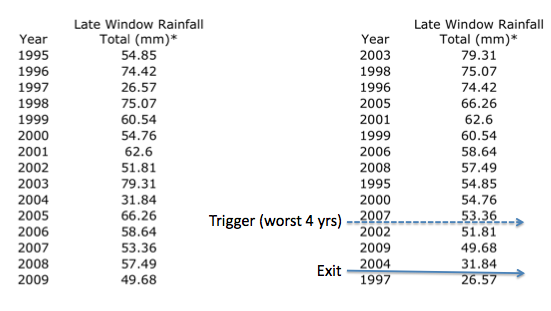
\includegraphics{chpt4imacheckans.png}
\end{figure}

This initial draft index sets the trigger and exit for a contract that would have paid out four times in the past fifteen years. Depending on the community reaction to the resulting payouts, the trigger and exit could be adjusted to reflect different types of payouts.  For example, if the trigger was set for the worst 5 years instead of the worst 4, then the contract will pay out more often, but note that this will also affect the premium (making the contract more expensive to purchase).  What the appropriate trigger and exit value should be is a process to be determined through interaction with the local community.

\textbf{Answers}
\begin{enumerate}
\setcounter{enumi}{2}
\item {} 
What is the Exit value for this contract? 27 mm

\end{enumerate}
\begin{enumerate}
\setcounter{enumi}{4}
\item {} 
Choose a value to Trigger the contract: 53 mm (There are multiple correct answers)

\end{enumerate}


\chapter{Exploring Technical Concepts Using Weather Index Insurance Educational Tool (WIIET)}
\label{index_updated_educationalMat:exploring-technical-concepts-using-weather-index-insurance-educational-tool-wiiet}

\section{WIIET Exercise 1: Updating an Index Using Farmer Information}
\label{wiiet/wiiet_usingfarmerinformation_Web:wiiet-exercise-1-updating-an-index-using-farmer-information}\label{wiiet/wiiet_usingfarmerinformation_Web::doc}

\subsection{Topic: Updating an Index Using Farmer Information}
\label{wiiet/wiiet_usingfarmerinformation_Web:topic-updating-an-index-using-farmer-information}

\subsubsection{Objective}
\label{wiiet/wiiet_usingfarmerinformation_Web:objective}
The goal of this exercise is to demonstrate how to adapt an initial drought index based on discussions with farmers.


\subsubsection{Introduction}
\label{wiiet/wiiet_usingfarmerinformation_Web:introduction}
Imagine that you are bringing a preexisting index to a new community. Discussions with the farmers will help you to determine if the index is useful for this new community and if it should be adjusted.

This exercise uses hypothetical indices and interviews for a hypothetical community. However, it is based on rainfall data, as well as modified versions of the indices and farmer discussions that have previously occurred in the R4 project, in Ethiopia.
\begin{description}
\item[{Weather Index Insurance Educational Tool (WIIET):}] \leavevmode
For this exercise we will be using the Weather Index Insurance Educational Tool (WIIET), pronounced ``wheat''. \emph{This tool can be accessed at:} \href{http://iri.columbia.edu/wiiet}{http://iri.columbia.edu/wiiet}. It is intended to teach the index design process for index-based insurance by allowing the user to create an index by working through a series of modules. In this way, the user is able to walk through the index design process step by step: from the collection of crop and climate information to selecting the index parameters; from tuning those index parameters to eventually evaluating the index''s performance. The end result is to have an index that successfully models and hedges against the climate risk that farmers face in real-world conditions and that offers protection at a price that is not prohibitively expensive.

\end{description}

In the following exercises we will primarily focus on creating and pricing indices for drought index insurance. In the Create Contract module, you can create an index and apply it to a historical or simulated rainfall dataset to see what payouts would have occurred. The \emph{Pricing} module allows you to calculate an insurance premium that is based on the payouts calculated in the Create Contract module. \emph{If you need further clarification at any point during this exercise, please refer to the User Guide, which can be found by clicking on the respective icon at the top right of any WIIET page.}
\begin{description}
\item[{\textbf{Software note:}}] \leavevmode
We recommend the Firefox browser for these WIIET modules because it has been the most tested. The tool is designed to work with other browsers, however you may encounter some occasional ``bugs'' in the system. We are currently working to fix these kinks and have included work-arounds in this material. For example, depending on your specific browser, you may need to reload the page or return to the main menu to ensure saved datasets are visible for future activities.

\end{description}


\subsubsection{Exercise Overview}
\label{wiiet/wiiet_usingfarmerinformation_Web:exercise-overview}\begin{description}
\item[{\textbf{Background Information:}}] \leavevmode
Tasks 1 to 4, below, walk you through the following scenario: You are bringing a preexisting drought index to a new community to see if it is appropriate for them. Discussions with the farmers will help you to determine if the index is useful and if it should be adjusted. Using the computer web-tool, WIIET, you follow up on that discussion and develop a new drought index based on their responses, if necessary. After you have a new index, you will return to the farmers and discuss the strengths and weaknesses of your new index and if they want to move forward with the insurance process.

\end{description}

During the following exercises you will be working on creating an accurate drought index for a crop known as Teff. This crop is native to Ethiopia and similar to wheat. Teff, in this area, is planted in the middle of the rainy season, when there has always been enough rain (according to the rainfall data and the farmers' memories). This crop is primarily vulnerable to lack of rainfall at the end of the season. Thus, the Teff index only focuses on the end of the rainfall season.

This exercise is focused on information provided by the farmers because it is the most important part of the process. Future exercises will use scientific analysis tools to further validate the indices. These include crop water stress calculations, and statistical modeling of rainfall. It is possible to use advanced modeling to validate and improve these indexes. The indices that you will create in these exercises are designed to reflect the information contained in the sophisticated models in a way that can also leverage information from farmers and experts. They are also structured to be as easy to understand as possible.
\begin{description}
\item[{\textbf{Initial Index Information:}}] \leavevmode
The information for the preexisting index is below. Task 1 will walk you through how to enter this information into WIIET. This will serve as a starting point for your new index:

\end{description}
\begin{itemize}
\item {} 
Contract start date: 11 August

\item {} 
Length: 70 days

\item {} 
Cap: 25

\item {} 
Index Trigger: 82

\item {} 
Index Exit: 60

\item {} 
Payout Years  (Since 1995): 1995, 1997, 2000, 2004, 2008

\end{itemize}


\subsection{Task 1: Bringing a preexisting index to a nearby community}
\label{wiiet/wiiet_usingfarmerinformation_Web:task-1-bringing-a-preexisting-index-to-a-nearby-community}
\emph{Note: Now we are going to put this existing information into the computer:}
\begin{enumerate}
\item {} 
Log on to WIIET. Go to: \href{http://iri.columbia.edu/wiiet}{http://iri.columbia.edu/wiiet} and enter your assigned user name and password (or create a new account, if one has not been provided)

\item {} 
Go to \textbf{Create Contract} module on the left hand side of the page

\item {} 
Click on Example Satellite Precipitation in the Step 1 window on the left, to select that rainfall dataset

\item {} 
In the \emph{Step 2} window it asks, ``When would you like the contract to begin?'' Click on \textbf{Contract Start Dekad} and set the contract start dekad as: 11-Aug. (If you are using Internet Explorer 8, you may have difficulty with this step. A temporary work around for this is to click on \textbf{Contract Start Window} and then select a \emph{Start of Aug 11} and an \emph{End of Sept 1.} The \emph{Contract Start Requirements} should be set to \emph{0 mm.} We are in the process of fixing this bug.)

\item {} 
\emph{Length of Contract Period:} select \textbf{7} dekads

\item {} 
At the bottom of the Step 2 box there is a matrix referring to phases covered. Click on the remove phase button until you have only \textbf{Phase 1.} Next, make sure each of the circles in that phase are blue by clicking on them.

\item {} 
Under \emph{Step 3} you can set the \emph{Dekadal Cap} to \textbf{25.} The use of a cap is further described in Module 1.

\item {} 
Set the Contract Failed Start Liability to \textbf{100.} This is not applicable for the index you are using. For some more complicated indices this is the payout if sowing conditions are not met.

\item {} 
On the bottom most table, set the \emph{Trigger} to \textbf{82.}

\item {} 
Set the \emph{Exit} to \textbf{60.}

\item {} 
Set the \emph{liability} for the phase to \textbf{100.}  This is the maximum payout for each individual phase.  Assume this means that the maximum payout is 100 dollars.  Because we have chosen 100, this means that the payouts reported by the software can be thought of either in terms of dollars or in terms of percentage.

\item {} 
Set the \emph{Maximum liability} to \textbf{100.} This is the total amount of money insured (100 percent) across all phases.  Because there is only one phase in our simple contract, this simply is the maximum liability of the individual phase.  For contracts with multiple phases, this parameter becomes more important.

\item {} 
Now you are ready to \textbf{Run Simulation:} Click on the bottom right side of the page

\item {} 
Once you get results (a Payout Calculation graph and table), click on \textbf{`save parameters',} in blue on the left hand side of the screen.  Use the name: \textbf{``original'',} and description \textbf{``original index''.} Then click \textbf{save.} Then click \textbf{close.}

\end{enumerate}

\textbf{Interpreting the Results:} The graph and table you see on your screen are the results of applying this preexisting drought index in the new community. The graph shows what years would have paid out historically and the size of the payout you would have received if you had gotten the rainfall for that year. Because we have set the maximum payout to \$100, you can think of this either as dollars or percentage of maximum payout. Because WIIET is designed to work with many different kinds of indices, some of the data presented will not be meaningful for the simple index we are working with for this exercise.

The resulting table has 5 columns: ``Harvest Year'' is the year that the data reflects, according to the year in which the crop would have been harvested. The ``Sowing Dekad'' is the number of the dekad, or approximate ten-day period when the contract began.  There are 360 dekads in a year.  For example, dekad 23 means that the index started in the 23rd dekad of the year, or the 11th of August.  For some more complex indices, this date changes from year to year, depending on the rainfall that year. The ``Rainfall for Phases''- total adjusted rainfall for the index window after the dekadal cap is applied for each phase. The ``Payout for Phases'' is the payout that would occur for each phase of the contract.  The ``Total Payout'' - total payout accounting for every phase (in this example there is only one phase, so this is the same as the ``Payout for Phase'').

\textbf{Questions:}
\begin{enumerate}
\item {} 
What years would have paid out? \_\_\_\_\_\_\_\_\_\_\_\_\_\_\_\_\_\_\_\_\_\_\_\_\_\_\_\_\_\_\_\_\_\_\_\_\_\_\_\_\_\_\_\_\_\_\_\_\_\_\_\_\_\_\_\_\_\_\_\_\_\_

\item {} 
How many payouts would there have been? \_\_\_\_\_\_\_\_\_\_\_\_\_\_\_\_\_\_\_\_\_\_\_\_\_\_\_\_\_\_\_\_\_\_\_\_\_\_\_\_\_\_\_\_\_\_\_\_\_\_\_\_\_\_\_\_\_\_\_\_\_

\item {} 
Are there any years with full payouts? If Yes, how many? \_\_\_\_\_\_\_\_\_\_\_\_\_\_\_\_\_\_\_\_\_\_\_\_\_\_\_\_\_\_\_\_\_\_\_\_\_\_\_\_\_\_\_\_\_\_\_\_\_\_\_\_\_\_\_\_\_\_\_\_\_\_\_\_\_\_\_\_\_\_\_\_\_\_\_

\end{enumerate}


\subsection{Task 2: Adjusting the drought index based on farmer input}
\label{wiiet/wiiet_usingfarmerinformation_Web:task-2-adjusting-the-drought-index-based-on-farmer-input}
\textbf{Context:} Now, imagine you have just returned from your trip to the new community. Below are the notes you took from your discussion with the new farmers.
\begin{itemize}
\item {} 
Dates; start: 21 August

\item {} 
Length of desired insurance: 40 days

\item {} 
Bad years from farmers: 2000, 2004, 2006, 2007, 2009

\item {} 
Very bad years from farmers: 2000, 2004, 2009

\item {} 
Crops desired to be insured: Teff

\end{itemize}

\textbf{The steps outlined here will help you take their feedback into account:}
\begin{enumerate}
\item {} 
Compare the information that the farmers in the new community gave you to the results that the WIIET tool generated. \emph{Note that the difficult years described by the farmers do not completely agree with the existing contract that you designed.}

\item {} 
Next you will try to make a more appropriate index to fit the farmers'' needs. The below steps will help you make these adjustments. \emph{You will need to adjust the} \textbf{start date} and \textbf{length} of insurance to \emph{better match the farmer's concerns:}

\end{enumerate}
\begin{itemize}
\item {} 
To navigate back so you can adjust the information you previously entered, click on \textbf{``view parameters''} at the top of the screen.

\item {} 
Change the contract to reflect the \textbf{start} and \textbf{length} the farmers reported. This means reentering these two numbers, using the new information given above. Remember to translate the \emph{length} given into dekads (10 day periods).

\item {} 
Then, click on \textbf{``Run Simulation''} at the bottom.

\end{itemize}

\textbf{Questions:}
\begin{enumerate}
\item {} 
How many payouts would this community have experienced in the last 15 years if this new index had been used? \_\_\_\_\_\_\_\_\_\_\_\_\_\_\_\_\_\_\_\_\_\_\_\_\_\_\_\_\_\_\_\_\_\_\_\_\_\_\_\_\_\_\_

\item {} 
Is this a realistic index?  \_\_\_\_\_\_\_\_\_\_\_\_\_\_\_\_\_\_\_\_\_\_\_\_\_\_\_\_\_\_\_\_\_\_\_\_\_\_\_\_\_\_\_\_\_\_\_\_\_

\item {} 
What else can be adjusted to create a better index that also addresses the farmers'' concerns? \_\_\_\_\_\_\_\_\_\_\_\_\_\_\_\_\_\_\_\_\_\_\_\_\_\_\_\_\_\_\_\_\_\_\_\_\_\_\_\_\_\_\_\_\_\_\_\_\_

\end{enumerate}


\subsection{Task 3: Making a More Appropriate Index}
\label{wiiet/wiiet_usingfarmerinformation_Web:task-3-making-a-more-appropriate-index}
\textbf{Context:} In this section you will adjust the \emph{trigger} and \emph{exit} until you have \textbf{5 payouts,} one of which is approximately a full payout. This will be a complicated process and you will probably need several tries.

The goal is to try to have as many payout years agree with the farmers as possible.  Try to not have too many very small payouts or very large payouts. However, it is impossible to do both of these things perfectly.

\emph{Hint: You may always switch between the ``view parameters'' screen and the ``view results'' screen by clicking on the gray bars at the top or bottom of the page. However, each time that you enter in new parameters you must hit the ``run simulation'' button in order to calculate your new index and historical payouts.}

\textbf{Now it is time for you to adjust and play with the exit and trigger values.} If you need some additional guidance, the ``Hint'' at the very end of this Task may be useful. Once you have some results to be proposed, click on \textbf{`save parameters'.} Use the name: \emph{``draft'',} and description \emph{``draft index''.}

\textbf{Questions:}
\begin{enumerate}
\item {} 
What trigger value have you chosen? \_\_\_\_\_\_\_\_\_\_\_\_\_\_\_\_\_\_\_\_\_\_\_\_\_\_\_\_\_\_\_\_\_\_\_\_\_\_\_\_\_\_\_\_\_\_\_\_\_\_\_\_\_\_\_\_\_\_\_\_\_\_\_

\item {} 
What exit value have you chosen? \_\_\_\_\_\_\_\_\_\_\_\_\_\_\_\_\_\_\_\_\_\_\_\_\_\_\_\_\_\_\_\_\_\_\_\_\_\_\_\_\_\_\_\_\_\_\_\_\_\_\_\_\_\_\_\_\_\_\_\_\_\_\_

\end{enumerate}

\textbf{Hint:}
\emph{Look at the ``rain by phase'' column of the output to decide what the trigger and exit should be. If the trigger is higher than the rain by phase for a particular year, that year will have a payout. If you want five payouts, you can find a trigger that has five years in which the rain by phase is less than that number. A full payout occurs when the exit is above the rain by phase. To have one year with a full payout, you can set the exit close to the lowest rain by phase value.}


\subsection{Task 4: Farmer discussion follow-up notes}
\label{wiiet/wiiet_usingfarmerinformation_Web:task-4-farmer-discussion-follow-up-notes}
\textbf{Context:} Now that you have your improved adjusted index (from Task 3), you have returned to the community to present it to the farmers. During this discussion they tell you that they want an index that would have paid more money in years like 2009. It is important to explain to the farmers that this would probably lead to an index that costs much more because all payouts would be much larger. The farmers should also be reminded that the future will be different from the past. The farmers understand your concerns; however, they are confident that the expense is worthwhile if payments in years like 2009 could be increased.

\textbf{In response, you must work with WIIET again to increase payout sizes, without impacting the number of payouts.} Return to adjust your parameters once again. Adjusting one single parameter can fulfill the farmers' request. Adjust and play with the parameter until you have an index that will satisfy the farmers.

\textbf{Questions:}
\begin{enumerate}
\item {} 
What parameter will you adjust to fulfill the farmers' request? \_\_\_\_\_\_\_\_\_\_\_\_\_\_\_\_

\item {} 
Will this number be increased or decreased? \_\_\_\_\_\_\_\_\_\_\_\_\_\_\_\_\_\_\_\_\_\_\_\_\_\_\_\_\_\_

\item {} 
Will this result in a more expensive index? Why or why not? \_\_\_\_\_\_\_\_\_\_\_\_\_\_\_\_\_\_\_ \_\_\_\_\_\_\_\_\_\_\_\_\_\_\_\_\_\_\_\_\_\_\_\_\_\_\_\_\_\_\_\_\_\_\_\_\_\_\_\_\_\_\_\_\_\_\_\_\_\_\_\_\_\_\_\_\_\_\_\_\_\_\_\_\_\_\_\_\_

\end{enumerate}


\section{WIIET Exercise 2: Influence of Short Datasets on Prices (Advanced Exercise)}
\label{wiiet/wiiet_influenceshortdatasets_Web::doc}\label{wiiet/wiiet_influenceshortdatasets_Web:wiiet-exercise-2-influence-of-short-datasets-on-prices-advanced-exercise}

\subsection{Topic: Influence of Short Datasets on Prices (Advanced Exercise)}
\label{wiiet/wiiet_influenceshortdatasets_Web:topic-influence-of-short-datasets-on-prices-advanced-exercise}

\subsubsection{Objective}
\label{wiiet/wiiet_influenceshortdatasets_Web:objective}
The goal of this exercise is to illustrate how shorter datasets can lead to increased insurance prices, as well as to illustrate some trade-offs between historical burn analysis and using simulated rainfall. This module is intended to follow WIIET Exercise 1: Updating an index using farmer information.


\subsubsection{Introduction}
\label{wiiet/wiiet_influenceshortdatasets_Web:introduction}
For further clarification or a more detailed description of the WIIET terms and tools, please refer to the \textbf{User Guide} or \textbf{Glossary.} Both can be found by clicking on their respective icons on any of the WIIET pages.

This module uses hypothetical indices and datasets. However, it is based on rainfall data and modified versions of the indices from the R4 project, in Ethiopia.

\textbf{Software note:} As stated in Exercise 1, it is ideal to complete these WIIET modules using the Firefox browser. The tool is designed to work with other browsers, however you may encounter some occasional ``bugs'' in the system. We are currently working to fix these kinks and have included work-arounds in this material. For example, depending on your specific browser, you may need to reload the page or return to the main menu so that saved datasets are visible for future activities.


\subsubsection{Exercise Overview}
\label{wiiet/wiiet_influenceshortdatasets_Web:exercise-overview}
\textbf{Background Information:} In the previous exercise, you updated a contract by focusing on historical precipitation data and farmer experiences. The focus on historical data had many benefits. It allowed you to understand the index, communicate it to the farmers, and modify the index to reflect their experiences. In addition, it prevented you from relying on complex statistical models, which may have limitations of which you are not aware and may generate unrealistic results based on model assumptions and structure (see \href{http://iri.columbia.edu/publications/id=875}{http://iri.columbia.edu/publications/id=875} p52-56 for more information).

However, there are several limitations of using historical data alone: One limitation is that possible rainfall for the coming year is confined to rainfall amounts exhibited in the historical data. This makes it impossible to have rainfall amounts that are different from what was experienced in the past. This limitation can lead you to accidentally over-fit to the historical data. In other words, it can create indices that are too tailored to particular events of the past to be flexible enough to address the wide range of possibilities that may occur in the future.

Another limitation with using historical data alone is that it does not provide you with the tools to address important questions that statistical modeling of rainfall can help you understand. We will focus on one such question: How do very short historical datasets impact insurance prices?


\subsection{Task 1: Set-up; historical rainfall data set}
\label{wiiet/wiiet_influenceshortdatasets_Web:task-1-set-up-historical-rainfall-data-set}
\textbf{In WIIET Exercise 1, you should have entered, run and saved the results from the ``original'' index.} If you have already performed these steps, you can always navigate back to your saved parameters by navigating the ``saved parameter sets'' drop down menu in Step 2 of the ``Create Contracts'' module.

\textbf{If you have not performed those steps, you can do so by following the instructions below} (The definitions for the terms used here are provided in earlier Exercises, as well as in the WIIET Glossary):
\begin{enumerate}
\item {} 
Log on to WIIET

\item {} 
Go to \textbf{create contract} module on the left hand side of the page

\item {} 
Click on \textbf{Example Satellite Precipitation} in the \emph{Step 1} window on the left, to select that rainfall dataset

\item {} 
In the \emph{Step 2} window it asks ``When would you like the contract to begin? Click on \textbf{Contract Start Dekad} and set the contract start dekad as: 11-Aug

\item {} 
\emph{Length of Contract Period:} select \textbf{7} dekads

\item {} 
At the bottom of the \emph{Step 2} box there is a matrix referring to \emph{phases} covered. Click on the remove phase button until you have only \textbf{Phase 1.} Next, make sure each of the circles in that phase are blue by clicking on them.

\item {} 
Under \emph{Step 3} you can set the \emph{Dekadal Cap} to \textbf{25}

\item {} 
Set the Contract Failed Start Liability to \textbf{100}

\item {} 
On the bottom most table set the \emph{Trigger} to \textbf{82}

\item {} 
Set the \emph{Exit} to \textbf{60}

\item {} 
Set the \emph{liability} for the phase to \textbf{100}

\item {} 
Set the \emph{Maximum liability} to \textbf{100}

\item {} 
Now you are ready to Run Simulation: Click on the bottom right side of the page

\item {} 
Once you get these results, click on \textbf{`save parameters',} in blue on the left hand side of the screen.  Use the name: \textbf{``original'',} and description \textbf{``original index''.} Then click \textbf{save.} Then click \textbf{close.}

\end{enumerate}


\subsection{Task 2: Thinking about simulated rainfall}
\label{wiiet/wiiet_influenceshortdatasets_Web:task-2-thinking-about-simulated-rainfall}
\textbf{Discussion:} Using historical data to design and evaluate your contract is known as `historical burn' analysis. It is extremely transparent and can be easily communicated to stakeholders. In historical burn analysis, the probability distribution of the indexed parameter is determined entirely by past measurements. Although useful, when applied without other analyses this approach has limitations. For example, one or two major events can distort the index design, while any event that has not happened in the historical record is assumed to not be possible for the coming year.

Due to the limitations of historical burn analysis, it is typically complimented with rainfall modeling and simulation. Using available rainfall data plus an understanding of the variables that influence rainfall, the modeling generates hundreds of years of synthetic rainfall data, including events that are possible but have not occurred in the past. This approach can be helpful in exploring limited datasets, allowing for more accurate estimates of diagnostics for index performance, less idiosyncratic indices, and the potential to model the limitations of short datasets.

The \emph{Rainfall Simulator} module in WIIET will generate approximately one thousand years of rainfall data based on the statistical properties of the precipitation data set selected. This module is useful in places where there is very little historical rainfall data because it uses methods that automatically build in additional variation in the rainfall to reflect increased uncertainty due to limited length of datasets.

The \emph{Rainfall Simulator} module estimates parameters of a statistical model for rainfall based on the observed data. When the model is used to generate random years of rainfall, the simulations are impacted by the amount of data used to fit the model. The model and its associated rainfall simulations account for (1) the natural variation in rainfall in that climate, and (2) the uncertainty in the estimation of the climate due to the limited length of the historical dataset. Accounting for this uncertainty adds extra variability to the simulated rainfall years.

How is this done? As with any statistical estimation, when the parameters of the rainfall model are estimated, the process results in standard errors, which reflect how confident we are in the accuracy of our estimates. For a short rainfall time series, the standard errors will most likely be larger, reflecting less information. As the number of years of observed rainfall increases, standard errors tend to decrease, reflecting the higher accuracy of estimation. The standard errors of the parameters therefore reflect the set of possible parameters that may identify the true range of potential rainfall amounts.

After the parameters and standard errors of the rainfall model are estimated, the model produces rainfall for the generation of random years by 1) randomly selecting parameters to run the rainfall model from the range determined by the standard errors from the estimation. 2) Randomly selecting rainfall amounts for a model using the chosen parameters. This process repeats hundreds and hundreds of times to ensure the generation of a wide range of possible rainfall amounts for the range of possible climates.

There are many situations in which a rainfall simulator does not accurately reflect true rainfall statistics, so you should always view results from any rainfall simulator with a critical eye. In order to reach acceptable performance and reliability, the simulator models rainfall over 10 day periods instead of modeling daily rainfall. Also, this model only reflects the spread of possible climates expressed in the statistical uncertainty of the rainfall model estimation; other sources of climate uncertainty are not incorporated in the model.

Because the rainfall is generated randomly, each time you run the module, the results are slightly different. Although it is possible for you to generate simulated rainfall datasets yourself using the Rainfall Simulator module, we have generated a set of simulated rainfall datasets so everyone in the workshop uses identical data to complete this exercise.

\textbf{Questions: (Based on the Discussion above)}
\begin{enumerate}
\item {} 
Does the rainfall in years generated by the rainfall simulator have more variation in rainfall than the historical record or less?  Why or why not?

\end{enumerate}


\subsection{Task 3: Applying a simulated rainfall dataset}
\label{wiiet/wiiet_influenceshortdatasets_Web:task-3-applying-a-simulated-rainfall-dataset}
\textbf{Context:} In WIIET Exercise 1, you generated payouts for a particular index using the historical rainfall data. Now you will generate a set of payouts using the simulated rainfall dataset. In both cases, for the sake of index design, you are assuming that the upcoming year will be one of the years in the rainfall dataset. Let's see how our understanding of the index changes as we use the simulated rainfall.

We have already created a simulated dataset for you entitled \emph{``Full dataset simulated rainfall''.} This dataset was created through the ``Rainfall Simulator'' module, using the same rainfall data that you used in the first Task. It is possible for you to create your own simulated dataset, but it can take a few minutes for the server to simulate 1,000 years of rainfall data; therefore we will not complete that task during this module.

\textbf{First, we need to generate a new set of payouts using the simulated rainfall dataset and the parameters that you already entered, so we can compare results.}
\begin{enumerate}
\item {} 
Go to \textbf{create contract} module on the left hand side of the page

\item {} 
Click on \textbf{Full dataset simulated rainfall} in the \emph{Step 1} window on the left to select the new, simulated rainfall dataset

\item {} 
In the \emph{Saved Parameter Sets} window click on \textbf{original,} the index you have already created

\item {} 
Now you are ready to \textbf{Run Simulation:} Click on the bottom right side of the page

\item {} 
The simulation will take longer this time, because it is processing about a thousand years of data. The payout year table and figure will now have about a thousand elements, with the simulation years beginning with year 1.

\item {} 
Once you get these results, click on \textbf{`save parameters',} in blue on the left hand side of the screen.  Use the name: \textbf{``fullsimulation-original'',} and description \textbf{``simulation using full historical dataset, original index''.} Then click \textbf{save.} Then click \textbf{close.}

\end{enumerate}


\subsection{Task 4: Historical verses simulated rainfall data}
\label{wiiet/wiiet_influenceshortdatasets_Web:task-4-historical-verses-simulated-rainfall-data}
\textbf{Context:} Now we will compare the effects of using historical data versus simulated rainfall data on the variance in payouts, our estimation of how frequently payouts will occur, and the implications this has for premium pricing. We will use the ``Pricing'' module of WIIET for this analysis to generate a `pseudo' risk price that can be used to understand how risk might impact final insurance prices.

\textbf{Discussion:} The intent of the risk price is to allow the designer to model risk protection and insurance cost tradeoffs sufficiently to make quality design decisions. You should be aware that it is a working price for design purposes and is likely to be somewhat different than the final price of a transacted contract. The actual price of the insurance will most likely be negotiated between the project stakeholders, and may be calculated using different formulas than those built into the pricing module. Often, prices are driven by proprietary analysis done by the insurance companies. Insurance costs have additional components, including the administrative costs of providing insurance and the delivery costs of registering clients and distributing their payouts. The actual price of the insurance tends to be higher than the risk prices you calculate here, due to these additional costs.

\textbf{Questions:}
\begin{enumerate}
\item {} 
Will insurance prices be higher than the risk prices you calculate using WIIET? \_\_\_\_\_\_\_\_\_\_\_\_\_\_\_\_\_\_\_\_\_\_\_\_\_\_\_\_\_\_\_\_\_\_\_\_\_\_\_\_\_\_\_\_\_\_\_\_\_\_\_\_\_\_\_\_\_\_\_\_\_\_\_\_

\item {} 
Why or why not? \_\_\_\_\_\_\_\_\_\_\_\_\_\_\_\_\_\_\_\_\_\_\_\_\_\_\_\_\_\_\_\_\_\_\_\_\_\_\_\_\_\_\_\_\_\_\_\_\_\_\_\_\_\_\_\_\_\_\_\_\_\_\_\_\_\_\_\_\_\_\_\_\_\_\_\_\_\_\_\_\_\_\_\_\_\_\_\_\_\_\_\_\_\_\_\_\_\_\_\_\_\_\_\_\_\_\_\_\_\_\_\_\_\_\_\_\_\_\_\_

\item {} 
What is the purpose of calculating risk prices using WIIET? \_\_\_\_\_\_\_\_\_\_\_\_\_\_\_\_\_\_\_\_\_\_\_\_\_\_\_\_\_\_\_\_\_\_\_\_\_\_\_\_\_\_\_\_\_\_\_\_\_\_\_\_\_\_\_\_\_\_\_\_\_\_\_\_\_\_\_\_\_\_\_\_\_\_\_\_\_\_\_\_\_\_\_\_\_\_\_\_

\end{enumerate}


\subsection{Task 5: Risk Pricing}
\label{wiiet/wiiet_influenceshortdatasets_Web:task-5-risk-pricing}
\textbf{Discussion:} The risk component of the price of insurance is driven by the expense of the financing necessary to assure payouts, estimated using the best information on the likelihood and size of a payout in the coming year.

There are two components to the risk price:
\begin{enumerate}
\item {} 
The first is simply the average payout. The insurance premium must be sufficient to cover the average amount of money being paid out. If \$100 is paid by the insurance about 1/10 of the time, the premium must be at least \$10.

\item {} 
In addition to the average payout, the insurance company must maintain sufficient capital on hand to be able to cover extreme payouts. Insurance companies will choose (or be required by regulations) to keep sufficient liquidity to honor payouts and must pay interest on this money, which contributes to the risk cost of the premium.

\end{enumerate}

Commonly, the money for extreme payouts is borrowed from the insurance company's shareholders, so the interest paid is the return on the shareholders' investment in the company. This money is held specifically to manage risk, as opposed to being put into investments (such as agricultural inputs) that would provide returns through production.

Often, insurance companies hold enough money to cover their best estimate of the largest payout they anticipate happening in 100 years. In our case, we know that a full payout is the maximum payout, and it is likely to happen multiple times in 100 years, because it would have happened in the past 15 years.

Holding enough money to cover extreme events is a fundamental cost of risk management. An individual farmer faces a similar choice whether she purchases insurance, maintains savings `for a rainy day', or borrows to cover losses after the drought has occurred. It is the basic tradeoff of how much money to keep liquid in case there is drought versus the money that is put at risk for higher returns by investing in inputs to a productive activity that may experience a loss.

From a risk financing perspective, the key difference between the insurance company and the farmer is that the insurance company can build a large portfolio of unrelated (or even opposite) risks. This way the amount of money that must be held is less than the farmer would have to reserve. Premiums received each year by the insurance company can also be used as payouts that year, reducing the amount of money that must be borrowed.

For this exercise, the calculation of the ``pseudo price'' for risk is below.

Price = Average payout including zero payout years + \textbf{cost of capital} * (Maximum Payout - average payout)

\emph{In WIIET the ``cost of capital'' is labeled ``loading''}

\textbf{To use the pricing module of WIIET to analyze the payout information, follow the steps below} (The definitions for the terms used here are provided in previous educational and WIIET exercises, as well as in the WIIET Glossary):

\textbf{A. Risk Pricing for Historical Rainfall}
\begin{enumerate}
\item {} 
Go to \textbf{Pricing} module (tab on top of page, or if you just logged in, just below the create contract module).

\item {} 
Click on \textbf{original} in the Payout Data Series window of Step 1, on the left. Now you have selected the payouts you calculated already for the original contract using the historical rainfall dataset.

\item {} 
Set the \emph{Maximum Liability} to \textbf{100.} This is the total amount of money insured, \$100 across all phases. This is to reflect the amount you set when you create the contract.

\item {} 
Set the \emph{Value at Risk} to \textbf{1}. This tells the pricing software that the money to hold to should be enough to pay the entire maximum liability.

\item {} 
Set the \emph{Loading} (cost of capital) to \textbf{0.10.}  This means that the insurance company must pay ten percent interest on the money it borrows to honor large payouts.

\item {} 
Click on \textbf{Run,} on the bottom right, to see the results.

\item {} 
Once you are satisfied with the results, click on \textbf{Print/View,} on the left hand side of the page. The results will open in a new window.

\end{enumerate}

\textbf{Interpreting the Results:} When you run the pricing module, it makes a table of calculated numbers. While not all of these numbers are informative for our current exercise, a description of each value is provided below:

The \emph{Maximum Payout} is the largest payout that occurred in the data set. In this exercise, the largest possible maximum payout is set to be 100, so you can think of the payout values as a percentage.

The price is presented in two ways: \emph{Premium in Cash} provides the actual amount of money that will be charged for active insurance coverage based on the risk price formula. Because the maximum payout is \$100, this will be identical to the \emph{Premium as a percentage of sum insured,} which presents the price as a fraction of the maximum possible payout.

The \emph{Value of Loss at Value at Risk Percentile} calculates the amount of money that the insurance company would need to cover the biggest payout anticipated.  We have conservatively set this to be the maximum payout.

The \emph{Payout Variance} is the statistical value of the variance in payouts from year to year. A larger value indicates a widely varied contract, whereas a smaller value indicates a contract for which the payout does not vary greatly from year to year.

The \emph{Mean} (average) \emph{payout} is the total of all the payouts divided by the number of years in the data set. The \emph{Number of years} is the number of years in the data set, while the \emph{Number of payouts} over the course of these years is also presented in the table.

\textbf{Questions:}
\begin{enumerate}
\item {} 
What is the risk premium of the original contract calculated using the historical data?  \_\_\_\_\_\_\_\_\_\_\_\_\_\_\_\_\_\_\_\_\_\_\_\_\_\_\_\_\_\_\_\_\_\_\_\_\_\_\_\_\_\_\_\_\_\_\_\_\_\_\_\_\_\_\_\_\_\_\_\_\_

\item {} 
What is the average payout? \_\_\_\_\_\_\_\_\_\_\_\_\_\_\_\_\_\_\_\_\_\_\_\_\_\_\_\_\_\_\_\_\_\_\_\_\_\_\_\_\_\_\_\_

\item {} 
Why is the premium higher than the average payout? \_\_\_\_\_\_\_\_\_\_\_\_\_\_\_\_\_\_\_\_\_\_\_\_\_\_\_\_\_\_\_\_\_\_\_\_\_\_\_\_\_\_\_\_\_\_\_\_\_\_\_\_\_\_\_\_\_\_\_\_\_\_\_\_\_\_\_\_

\end{enumerate}

\textbf{B. Risk Pricing for Simulated Rainfall}
\begin{enumerate}
\item {} 
Navigate back to adjust your parameters by clicking on the grey ``view parameters'' bar at the top of the screen.

\item {} 
Repeat the previous pricing steps above; however, this time use the \textbf{fullsimulation-original} payout data series (select this dataset under \emph{Payout Data Series).} This will allow you to compare the simulated rainfall payout results with the historical rainfall payout results you just calculated.

\item {} 
When you are done, click on \textbf{Print/View these results.} This will open a new window with the new results, so that you can compare the two sets of output. You may need to drag one window to the side so they do not completely cover each other. If you get confused about which window is which, you can look at the number of years, which will be 15 for the historical series and almost 1000 for the simulated series.

\end{enumerate}

\textbf{Questions:}
\begin{enumerate}
\item {} 
Which payout series has a higher risk price? \_\_\_\_\_\_\_\_\_\_\_\_\_\_\_\_\_\_\_\_\_\_\_\_\_\_\_\_\_\_

\item {} 
Why? \_\_\_\_\_\_\_\_\_\_\_\_\_\_\_\_\_\_\_\_\_\_\_\_\_\_\_\_\_\_\_\_\_\_\_\_\_\_\_\_\_\_\_\_\_\_\_\_\_\_\_\_\_\_\_\_\_\_\_\_\_

\item {} 
What is the payout rate for the simulated series (divide the number of payouts by the number of years)? \_\_\_\_\_\_\_\_\_\_\_\_\_\_\_\_\_\_\_\_\_\_\_\_\_\_\_\_\_\_\_\_\_\_\_\_\_\_\_\_\_\_\_\_\_\_\_\_\_\_\_\_\_\_\_\_\_\_\_\_\_\_\_

\item {} 
Is this higher or lower than the 30\% payout rate obtained when using the historical data series? \_\_\_\_\_\_\_\_\_\_\_\_\_\_\_\_\_\_\_\_\_\_\_\_\_\_\_\_\_\_\_\_\_\_\_\_\_\_\_\_\_\_\_\_\_\_\_\_\_\_\_\_\_\_

\item {} 
Why? \_\_\_\_\_\_\_\_\_\_\_\_\_\_\_\_\_\_\_\_\_\_\_\_\_\_\_\_\_\_\_\_\_\_\_\_\_\_\_\_\_\_\_\_\_\_\_\_\_\_\_\_\_\_\_\_\_\_\_

\end{enumerate}

\textbf{Advanced Question:}

Although the mean payout is higher for the simulated payout series (as would be expected), the variance in the payouts is actually lower. How is this possible and what does it say about the changes in payouts? \_\_\_\_\_\_\_\_\_\_\_\_\_\_\_\_\_\_\_\_\_\_\_\_\_\_\_\_\_\_\_\_\_\_


\subsection{Task 6: Length of dataset and risk price of insurance}
\label{wiiet/wiiet_influenceshortdatasets_Web:task-6-length-of-dataset-and-risk-price-of-insurance}
\textbf{Discussion:} Information quality impacts the fundamental cost of insurance. The premium must reflect the range of possible payouts that may occur. Otherwise, the insurance company cannot responsibly commit to honoring the insurance contract. As information improves about the probabilities of payouts, that information can reduce the cost of insurance, so that overly conservative levels of reserves and premiums are not required. Because the rainfall simulation module builds into the rainfall simulation the increased uncertainty about climate when using shorter datasets, we can explore the implications of having less data.

\textbf{Context:} The rainfall simulation you used in the previous calculations was based on the complete set of 15 years of historical data. To see how our calculations would change if we only had the past five years of data, we have also run the rainfall simulation using only the past 5 years of historical data. This is saved as Short dataset simulated rainfall.

\textbf{Complete the following steps:}
\begin{enumerate}
\item {} 
Go back to the \textbf{create contract} module. Calculate the payouts for this dataset using the original contract.  Select \textbf{Short dataset simulated rainfall} under the \emph{Precipitation Datasets} in \emph{Step 1.} Then select your \textbf{Original} contract in \emph{Saved Parameter Sets} under \emph{Step 2.}

\item {} 
Next click on \textbf{Run Simulation} at the bottom right of the screen.

\item {} 
Save these parameters as recentsimulation-original, by clicking \textbf{Save the parameters} on the left.

\end{enumerate}

\textbf{Go to the pricing module and run it using this payout series:}
\begin{enumerate}
\item {} 
Click \textbf{Pricing} at the top of the screen and navigate back to adjust your parameters.

\item {} 
Select \textbf{recentsimulation-original,} under the \emph{Payout Data Series} in \emph{Step 1.}

\item {} 
Your other parameters should remain the same as when you ran the pricing module before.

\item {} 
Click \textbf{Run} at the bottom right of the screen.

\end{enumerate}

\textbf{Questions:}
\begin{enumerate}
\item {} 
Is the payout rate (number of payouts/number of years) for the simulated rainfall series using the recent data series higher or lower than that of the simulated rainfall series using the full set of historical data? \_\_\_\_\_\_\_\_\_\_\_\_\_\_\_\_\_\_\_\_\_\_\_\_\_\_\_\_\_\_\_\_\_

\item {} 
Why? \_\_\_\_\_\_\_\_\_\_\_\_\_\_\_\_\_\_\_\_\_\_\_\_\_\_\_\_\_\_\_\_\_\_\_\_\_\_\_\_\_\_\_\_\_\_\_\_\_\_\_\_\_\_\_\_\_\_\_\_\_

\item {} 
Are the mean, variance, and price for the simulated rainfall series using the recent data series higher or lower than that of the simulated rainfall series using the full set of historical data? \_\_\_\_\_\_\_\_\_\_\_\_\_\_\_\_\_\_\_\_\_\_\_\_\_\_\_\_\_\_\_\_\_\_\_\_\_\_\_\_\_\_\_\_\_\_\_\_\_\_\_

\item {} 
Why? \_\_\_\_\_\_\_\_\_\_\_\_\_\_\_\_\_\_\_\_\_\_\_\_\_\_\_\_\_\_\_\_\_\_\_\_\_\_\_\_\_\_\_\_\_\_\_\_\_\_\_\_\_\_\_\_\_\_\_\_\_\_

\end{enumerate}

\textbf{Advanced Task:}

For additional comparisons, create a set of payouts using only the past five years of historical data (Recent Satellite precipitation). Save it as recenthistorical-original.  Then run the pricing module on this series.

\textbf{Questions:}

Can comparison of short and long historical datasets give you the information you got from earlier tasks comparing simulated rainfall? Why or why not? \_\_\_\_\_\_\_\_\_\_\_\_\_\_\_


\section{WIIET Exercise 3: Moving from Initial Pricing to Market Pricing}
\label{wiiet/wiiet_initialtomarketpricing_Web:wiiet-exercise-3-moving-from-initial-pricing-to-market-pricing}\label{wiiet/wiiet_initialtomarketpricing_Web::doc}

\subsection{Topic: Moving from Initial Pricing to Market Pricing}
\label{wiiet/wiiet_initialtomarketpricing_Web:topic-moving-from-initial-pricing-to-market-pricing}

\subsubsection{Introduction}
\label{wiiet/wiiet_initialtomarketpricing_Web:introduction}
This exercise illustrates the types of considerations that go into the index insurance pricing process. Participants will take on the role of the insurer/reinsurer. You will use historical rainfall data to calculate a historical risk price in WIIET, as a starting point for determining an appropriate market price of an index. Next, the historical rainfall data will be used to create a simulated rainfall dataset, as well as datasets that represent different climate scenarios. You will then calculate the risk price of these scenarios to see the range of risk prices that result. This analysis will help you get a better sense for the additional amount of uncertainty that should be added to your historical risk price. The exercise concludes by guiding you through combining your historical risk price, additional loading due to uncertainty, and administrative and business expenses to arrive at a final market price.

This Exercise has four Segments:

Segment 1: Advanced Statistical Analysis

Segment 2: Sensitivity Tests

Segment 3: Factoring in Uncertainty

Segment 4: Moving from Risk Pricing to Market Pricing: using spreadsheets

\emph{This module uses hypothetical indices and datasets. However, it is based on rainfall data and modified versions of the indices from the R4 project, in Ethiopia.}

\emph{When you are covering multiple indices their payouts average together, which makes it possible to lower the price of insurance. The portfolio analysis that is used to calculate this approach is beyond the scope of this exercise.}

\textbf{WIIET:} \emph{You can log on to WIIET by navigating to the following Web page:} \href{http://iri.columbia.edu/wiiet}{http://iri.columbia.edu/wiiet}. If you would like further clarification or a more detailed description of the WIIET terms and tools, please refer to the \emph{User Guide} or \emph{Glossary.} Both can be found by clicking on their respective icons on any of the WIIET pages.

As stated previously, it is ideal to complete WIIET activities using the Firefox browser. The tool is designed to work with other browsers, however you may encounter some occasional ``bugs'' in the system. We are currently working to fix these kinks and have included work-arounds in this material. For example, depending on your specific browser, you may need to reload the page or return to the main menu so saved datasets are visible for future activities.


\subsubsection{Exercise Overview}
\label{wiiet/wiiet_initialtomarketpricing_Web:exercise-overview}
\textbf{Background Information:} In WIIET Exercise II: Influence of Short Datasets on Prices, you explored how the increased uncertainty characteristic of shorter datasets leads to increased insurance prices. You did this by pricing contracts using a shortened dataset and a longer historical dataset, and then comparing your results. It also helped you begin to explore the trade-offs between historical burn analysis and using simulated rainfall. This pricing module is intended to follow and build upon WIIET Exercise II.

\textbf{Overview of important terms:}

\emph{Historical burn analysis} uses historical data to design and evaluate a contract. One of the greatest benefits of historical burn analysis is it is extremely transparent and can be easily communicated to stakeholders. Although useful, when applied without other analyses this approach has limitations; it sole relies on past events to determine the probability distribution of the indexed parameter. As a result, too much weight may be placed on a select few events in the historical record, while other possible events that have not occurred in the historical dataset will not be accounted for. This becomes even more limiting when you have a short historical dataset from which to reference.

On the other hand, \emph{simulated rainfall} expands upon the information provided by the historical rainfall dataset to provide a fuller picture of the rainfall events that may occur in the future.

\emph{Risk Pricing:} The intent of the risk price is to allow the designer to model risk protection and insurance cost tradeoffs sufficiently to make quality design decisions. The risk price provided in WIIET is a working price for design purposes and is likely to be somewhat different than the final price of a transacted contract.

The risk component of the price of insurance accounts for the amount of money necessary to cover any insurance payouts that may occur. The risk price is comprised of two parts: 1) the average payout. For example, the insurance premium must be sufficient to cover the average amount of money being paid out. If \$100 is paid by the insurance about 1/10 of the time, the premium must be at least \$10. 2) The liquidity necessary to cover extreme payouts; the insurance companies must be prepared to cover extreme events.

The Risk Price is determined using the following formula:
Risk Price = Average payout including zero payout years + cost of capital * (Maximum Payout - average payout)

\emph{In WIIET ``cost of capital'' is labeled ``loading''}

In WIIET the Risk Price is called ``Premium in Cash''.

While the risk price is a starting point for determining the price of an insurance contract, it does not account for all that needs to be included in a contract's price.  This exercise will help you understand some of the other factors you need to take into account when designing an index insurance contract and evaluating its price. The actual price of the insurance will, in general, be higher than the risk prices you calculate in WIIET, due to these additional costs.


\subsubsection{Task 1: Setup - Index Parameters}
\label{wiiet/wiiet_initialtomarketpricing_Web:task-1-setup-index-parameters}
Throughout this exercise we will be using the same index parameters in each Task. You can always navigate back to your saved parameters by navigating the ``saved parameter sets'' in the drop down menu under each module. Tasks 1, 2 and 3 are similar to the steps preformed in WIIET Exercise II, but are necessary to include here, as they will serve as the basis for our analysis moving forward. While these initial tasks may appear redundant they contain more advanced discussions that will be important throughout this exercise. Please, read over each tasks even if it looks familiar.

In order to start this Educational Exercise and set up your parameters, follow the steps below:
\begin{enumerate}
\item {} 
\textbf{Access the WIIET tool by navigating to} \href{http://iri.columbia.edu/wiiet}{http://iri.columbia.edu/wiiet}. Use the username and password you were provided.

\item {} 
\textbf{If you have completed Exercise I or II and saved your results:} you do not have to repeat the setup steps below. Your index parameters should already be saved as ``original'' and you can skip to Task II. However, it may be helpful to read over these steps to refresh your memory.

\item {} 
Work in \textbf{Create Contracts:} (The definitions for the terms used here are provided in Exercises I and II, as well as in the WIIET Glossary):
\begin{itemize}
\item {} 
Go to \textbf{create contract} module on the left hand side of the page

\item {} 
Click on \textbf{Example Satellite Precipitation} in the \emph{Step 1} window on the left, to select that rainfall dataset

\item {} 
In the \emph{Step 2} window it asks ``When would you like the contract to begin?'' Click on \textbf{Contract Start Dekad} and set the contract start dekad as: 11-Aug

\item {} 
\emph{Length of Contract Period:} select \textbf{7} dekads

\item {} 
At the bottom of the \emph{Step 2} box there is a matrix referring to \emph{phases} covered. Click on the remove phase button until you have only \textbf{Phase 1.} Next, make sure each of the circles in that phase are blue by clicking on them.

\item {} 
Under \emph{Step 3} you can set the \emph{Dekadal Cap} to \textbf{25}

\item {} 
On the bottom most table set the \emph{Trigger} to \textbf{82}

\item {} 
Set the \emph{Exit} to \textbf{60}

\item {} 
Set the \emph{liability} for the phase to \textbf{100}

\item {} 
Set the \emph{Maximum liability} to \textbf{100}

\item {} 
Now you are ready to \textbf{Run Simulation:} Click on the bottom right side of the page.

\item {} 
Once you get these results, click on \textbf{`save parameters'}, in blue on the left hand side of the screen. Use the name: \textbf{``original''}, and description \textbf{``original index''}. Then click \textbf{save.} Then click \textbf{close.}

\item {} 
This generates payouts for the index using the historical rainfall data.

\end{itemize}

\end{enumerate}


\subsubsection{Task 2: Pricing of Historical Rainfall Dataset}
\label{wiiet/wiiet_initialtomarketpricing_Web:task-2-pricing-of-historical-rainfall-dataset}
In this task you will start with 15 years of historical rainfall data (\textbf{``Example Satellite Precipitation''}) and use the ``original index'' parameters to calculate the price of the historical burn index in WIIET. We will call this the historical risk price.

To calculate this price, follow the below steps:
\begin{enumerate}
\item {} 
Navigate to the Pricing Module by using the tabs at the top of your screen.

\item {} 
Click on ``original'' in the Payout Data Series window of Step 1.  This selects the payouts you calculated for the original index using the historical rainfall.

\item {} 
\textbf{If you have completed Exercise II and saved your results:} select ``original'' from the Pricing Parameters window. This will ensure we are using the same set of pricing parameters that were created in Exercise II for each of our pricing tests. The set up of these parameters are explained below in steps 4 through 8, if you would like to refresh your memory. Next click on ``run'' on the bottom right to see the results. You do not need to repeat steps 4 through 8.

\item {} 
Set the \emph{Maximum Liability} to \textbf{100.} This is the total amount of money insured, \$100 across all phases. This is to reflect the amount you set when you create the contract.

\item {} 
Set the \emph{Value at Risk} to \textbf{1.} This tells the pricing software that the money to hold should be enough to pay the entire maximum liability.

\item {} 
Set the \emph{Loading} (cost of capital) to \textbf{0.10.}  This means that the insurance company must pay ten percent of the money it needs to have available to honor large payouts.

\item {} 
Click on ``run'' on the bottom right to see the results.

\item {} 
Save your pricing parameters under the title ``original''

\end{enumerate}

Interpreting Your Results: The \emph{Maximum Payout} is the largest payout that occurred in the dataset. For this exercise, the maximum possible payout is set to be 100 to enable you to think of payout values as a percentage. The risk price is presented in two ways: 1) \emph{Premium in Cash} and 2) \emph{Premium as percentage of sum insured.} The \emph{Premium in Cash} is the amount of money that will be charged for active insurance coverage based on the risk price formula. Since the maximum payout is \$100, the \emph{Premium as percentage of sum insured} will be identical to the \emph{Premium in Cash} value.

\textbf{Questions:}
\begin{enumerate}
\item {} 
What is the historical risk price (``premium in cash'')?\_\_\_\_\_\_\_\_\_\_\_\_\_\_\_\_\_\_\_\_\_\_\_\_\_\_

\item {} 
How many payouts occur using the historical rainfall dataset?\_\_\_\_\_\_\_\_\_\_\_\_\_\_\_\_\_\_\_\_

\item {} 
What is the average payout?\_\_\_\_\_\_\_\_\_\_\_\_\_\_\_\_\_\_\_\_\_\_\_\_\_\_\_\_\_\_\_\_\_\_\_\_\_\_\_\_\_\_\_\_\_\_\_\_\_\_\_\_\_\_\_\_

\item {} 
Does the maximum possible payout occur when using this dataset?\_\_\_\_\_\_\_\_\_\_\_

\item {} 
Why is the historical risk price higher than the average payout?\_\_\_\_\_\_\_\_\_\_\_\_\_\_\_\_\_\_\_\_\_\_

\item {} 
What is the payout variability?\_\_\_\_\_\_\_\_\_\_\_\_\_\_\_\_\_\_\_\_\_\_\_\_\_\_\_\_\_\_\_\_\_\_\_\_\_\_\_

\end{enumerate}

\textbf{Discussion:}

The historical burn price assumes that the only things that are possible for the coming year is exactly events that happened in the past historical dataset. Of course we know other things are possible, so we need to make sure we are anticipating those realistically. Perhaps the most challenging aspect of pricing insurance is determining the additional cost necessary to make sure the index responsibly captures uncertainties in the data and climate. In the next three Segments we will try to get an accurate picture of what this additional level of uncertainty might be.

There are two primary ways that insurance and reinsurance companies do this:
\begin{enumerate}
\item {} 
Advanced statistical analysis (Segment 1)

\item {} 
Sensitivity tests (Segment 2)

\end{enumerate}


\subsection{Segment 1: Advanced Statistical Analysis}
\label{wiiet/wiiet_initialtomarketpricing_Web:segment-1-advanced-statistical-analysis}
Advanced statistical analysis involves fitting available data to a statistical model in order to get a better understanding of the underlying statistical properties. By working with the statistical model, we are able to generate a more comprehensive dataset that includes events that have not occurred in the historical record, but that are likely to occur in the future, given what we know about the statistical properties of the historical data. We are also able to account for the limited information inherent in having a short dataset, by adding additional uncertainty into the model.

For these reasons, a dataset produced by a statistical model provides a good robustness test for our index. In other words, if the statistical analysis yields very different results than our historical burn analysis, it means our index may be too closely fit to the historical dataset and not adequately accounting for the full uncertainty we face. If the statistical analysis has results that are very similar to our historical burn analysis, this is a good first indicator that we have designed a robust index capable of addressing the nature of our risk.

The benefit to using a statistical model is it provides a systematic approach for analyzing data that can be repeated for new locations or as new information becomes available. Using such a systematic approach also lends itself to documentation that can be presented and explained to stakeholders, even if the concepts presented are less straightforward than the historical burn approach.

However, any model comes with its own set of limitations. By its very nature, a model is a simplification of real-world scenarios. Each statistical model is built to account for certain types of problems. To do this, the model must incorporate certain assumptions that may not always hold true in the real world. In a simplified world, where all the model's assumptions hold true, the price garnered from the statistical analysis would be the correct price for the insurance package.

\textbf{Questions:}
\begin{enumerate}
\item {} 
Why do statistical models provide a good robustness test for our index? \_\_\_\_\_\_\_\_\_\_\_\_\_\_

\item {} 
What are the benefits of using statistical models in the pricing process? \_\_\_\_\_\_\_\_\_\_\_\_\_\_\_

\item {} 
What are the limitations of using advanced statistical analysis as a pricing method? \_\_\_\_\_\_\_\_\_\_\_\_\_\_\_

\item {} 
In what scenario would a statistical model provide the correct price for an insurance package? \_\_\_\_\_\_\_\_\_\_\_\_\_\_\_

\end{enumerate}


\subsubsection{Task 3: Simulated Rainfall}
\label{wiiet/wiiet_initialtomarketpricing_Web:task-3-simulated-rainfall}
In this task, we will use a rainfall simulator, a statistical model embedded in WIIET that was designed with index insurance development purposes in mind, to do a robustness check of the index. This task will give you the opportunity to carry out an advanced statistical analysis for your original contract. While it is possible for you to generate a dataset using the rainfall simulator yourself, for the sake of conserving time and ensuring each participant has an identical dataset, we have already done this step for you. The simulated rainfall dataset is available in your dataset menu in the Step 1 window. This is the same simulated rainfall dataset that is used in Exercise II.

To create a set of payouts using this simulated rainfall dataset and the ``original'' index parameters, please follow the instructions below \textbf{(If you have completed Exercise II and saved your results: you do not have to complete steps 1 through 6. Your payout data series using the simulated rainfall and the original index should already be saved as ``fullsimulation-original''):}
\begin{enumerate}
\item {} 
Go to \textbf{create contract} module on the left hand side of the page

\item {} 
Click on \textbf{Full Dataset Simulated Rainfall} in the \emph{Step 1} window on the left to select the new, simulated rainfall dataset

\item {} 
In the \emph{Saved Parameter Sets} window click on original, the index you have already created (and also used for Exercise I and II).

\item {} 
Now you are ready to \textbf{Run Simulation:} Click on the bottom right side of the page

\item {} 
The simulation will take longer this time, because it is processing about a thousand years of data. The payout year table and figure will now have about a thousand elements, with the simulation years beginning with year 1.

\item {} 
Once you get these results, click on \textbf{`save parameters'} in blue on the left hand side of the screen.  Use the name: \textbf{``fullsimulation-original'',} and description \textbf{``simulation using historical dataset, original index''.} Then click \textbf{save.} Then click \textbf{close.}

\end{enumerate}

\textbf{You will now price this index using the Pricing Module. To do this, follow the steps below:}
\begin{enumerate}
\item {} 
Navigate to the Pricing Module by using the tabs at the top of your screen.

\item {} 
Click on ``fullsimulation-original'' in the Payout Data Series window of Step 1.  This selects the payouts you calculated for the original index using the simulated rainfall dataset.

\item {} 
Select ``original'' from the Pricing Parameters window.  This will ensure we are using the same set of pricing parameters for each of our pricing tests.

\item {} 
Click on ``run'' on the bottom right to see the results.

\end{enumerate}

\textbf{Questions:}
\begin{enumerate}
\item {} 
What is the simulated rainfall risk price? \_\_\_\_\_\_\_\_\_\_\_\_\_\_\_

\item {} 
Is this higher or lower than the historical risk price calculated above? \_\_\_\_\_\_\_\_\_\_\_\_\_

\item {} 
What is the average payout? \_\_\_\_\_\_\_\_\_\_\_\_\_\_\_

\item {} 
Does the average payout increase or decrease compared to the historical burn index? \_\_\_\_\_\_\_\_\_\_\_\_\_\_\_

\item {} 
What is the payout variability? \_\_\_\_\_\_\_\_\_\_\_\_\_\_\_

\item {} 
Does the payout variability increase or decrease compared to the historical burn index? \_\_\_\_\_\_\_\_\_\_\_\_\_\_\_

\item {} 
Using just this analysis, do these results indicate that your historical burn index is robust? \_\_\_\_\_\_\_\_\_\_\_\_\_\_\_

\end{enumerate}


\subsection{Segment 2: Sensitivity Tests}
\label{wiiet/wiiet_initialtomarketpricing_Web:segment-2-sensitivity-tests}
By using statistical analysis, insurance and reinsurance companies can get a sense of what events are likely to occur in the real world and are given an idea of an appropriate price for the insurance. But since every statistical model has its limitations, it is important that we incorporate other forms of analysis into our pricing process to explore some of the possibilities that may lie outside of the model's scope. One way of doing this is through sensitivity tests, which we will explore in this section.

Sensitivity tests can be used to supply additional information about how dependent the index we've developed (and its price) is on the specific dataset we used in our design process. These tests involve applying a given index to a slightly altered dataset to see if the adjustments result in any changes to the price of the index. Usually these tests will reflect events that there is reason to believe will occur in the coming year. So, if climate scientists or farmers have noticed a shift in the length or timing of an area's rainy season and suspect it may continue, it would make sense to apply the index parameters to rainfall datasets that reflect the shift and see what happens.

Sensitivity tests help us determine if we've over-fit our index to our data.  If the performance and price of an index does not change much as you apply these tests then the index is fairly robust. However, if the outputs change significantly than you may want to see how you can improve the index to make it more robust.

In this section we will perform three sensitivity tests. These tests are not particularly sophisticated, and they do not inform you of exactly what you need to change in order to create a robust index. However, they are able to reflect several kinds of issues likely to affect your index price and give you a sense of how vulnerable your index is to such changes, no matter what the cause. In the following tasks you will see how vulnerable the index is to slightly less rainfall on average, or the rainy season occurring slightly earlier or later than would be expected.

\textbf{Questions:}
\begin{enumerate}
\item {} 
Why do insurance and reinsurance companies perform sensitivity tests? \_\_\_\_\_\_\_\_\_\_\_\_\_\_\_

\item {} 
What does it tell you if the price of your index changes dramatically when you perform a sensitivity test? \_\_\_\_\_\_\_\_\_\_\_\_\_\_\_

\item {} 
How does a robust index perform under sensitivity tests \_\_\_\_\_\_\_\_\_\_\_\_\_\_\_

\end{enumerate}


\subsubsection{Task 4:  Determining Sensitivity to a General Decrease in Rainfall}
\label{wiiet/wiiet_initialtomarketpricing_Web:task-4-determining-sensitivity-to-a-general-decrease-in-rainfall}
Is the index price sensitive to a general decrease in rainfall?

To answer this question, you will price the original index parameters using a dataset that has five percent less rainfall than the historical record. For your convenience, this dataset has already been uploaded into the database for use in this exercise. Before you can price the contract, you will need to create payouts for this dataset.

\textbf{Follow the instructions below to do so.}
\begin{enumerate}
\item {} 
Navigate to the \textbf{create contract} module using the tabs at the top of the page

\item {} 
Click on \textbf{Pricing Activity 5 percent less} in the \emph{Step 1} window on the left.  This dataset is a tweaked version of the satellite data you worked with in your initial task. It has been altered to make the rainfall five percent lower than what was observed by the satellite.

\item {} 
In the \emph{Saved Parameter Sets} window click on \textbf{original,} the same contract you used to evaluate the historical and simulated datasets.

\item {} 
Now you are ready to \textbf{Run Simulation:} Click on the bottom right side of the page

\item {} 
Once you get these results, click on \textbf{`save parameters'} in blue on the left hand side of the screen.  Use the name: \textbf{``decreasedrainfall-original'',} and description \textbf{``historical dataset decreased by five percent, original index''.} Then click \textbf{save.} Then click \textbf{close.}

\end{enumerate}

\textbf{Now you will price the contract using the set of payouts you have just calculated.  Do this by following the steps below.}
\begin{enumerate}
\item {} 
Navigate to the \textbf{pricing} module by using the tabs at the top of your screen.

\item {} 
Click on ``decreasedrainfall-original'' in the Payout Data Series window of Step 1.  This selects the payouts you just calculated for the original index using the dataset with the five percent lower rainfall.

\item {} 
Select ``original'' from the Pricing Parameters window. This will ensure we are using the same set of pricing parameters for each of our pricing tests.

\item {} 
Click on ``run'' on the bottom right to see the results.

\end{enumerate}

\textbf{Questions:}
\begin{enumerate}
\item {} 
What is the risk price for the five percent less rainfall? \_\_\_\_\_\_\_\_\_\_\_\_\_\_\_

\item {} 
Is this higher or lower than the historical burn risk price? The simulated rainfall risk price? \_\_\_\_\_\_\_\_\_\_\_\_\_\_\_

\item {} 
How much did your average payout, number of payouts and payout variability change as compared to using the historical rainfall?  The simulated rainfall? \_\_\_\_\_\_\_\_\_\_\_\_\_\_\_

\item {} 
What does this tell you about your index's sensitivity to decreased rainfall? \_\_\_\_\_\_\_\_\_\_\_\_\_\_\_

\end{enumerate}


\subsubsection{Task 5: Determining Sensitivity to a Shift Forward in the Rainy Season}
\label{wiiet/wiiet_initialtomarketpricing_Web:task-5-determining-sensitivity-to-a-shift-forward-in-the-rainy-season}
Is the index price sensitive to the rainy season ending earlier?

To test this, you will price the original index parameters using another variation of the historical rainfall data; this data has been altered so that you are effectively starting and ending the rainy season one day earlier. While this may not sound like a significant change, because you are doing this to all the years you are changing the climate dramatically. This dataset is also provided in your dataset menu for the convenience of carrying out this exercise.  \textbf{Use the directions below to guide you through calculating payouts for this dataset.}
\begin{enumerate}
\item {} 
Return to the \textbf{create contract} module using the tabs at the top of the page

\item {} 
Click on \textbf{Pricing Activity 1 day fwd} in the \emph{Step 1} window on the left.  This dataset is an altered version of the satellite data you worked with in your initial task. In this dataset each year's rainy season begins and ends one day earlier than was the case in the historical record.

\item {} 
In the \emph{Saved Parameter Sets} window click on \textbf{original,} the same contract you used to evaluate the historical and simulated datasets.

\item {} 
Now you are ready to \textbf{Run Simulation:} Click on the bottom right side of the page

\item {} 
Once you get these results, click on \textbf{`save parameters.'} Use the name: \textbf{``earlyrainyseason-original'',} and description \textbf{``historical dataset shifted 1 day forward, original index''.} Click \textbf{save,} then \textbf{close.}

\end{enumerate}

\textbf{Now you will price the contract using the set of payouts you have just calculated.  Do this by following the steps below.}
\begin{enumerate}
\item {} 
Navigate to the \textbf{pricing} module using the tabs at the top of your screen.

\item {} 
Click on ``earlyrainyseason-original'' in the Payout Data Series window of Step 1.  This selects the payouts you just calculated for the original index using the dataset with the rainfall moved one day forward.

\item {} 
Select ``original'' from the Pricing Parameters window.  This will ensure we are using the same set of pricing parameters for each of our pricing tests.

\item {} 
Click ``run'' to see the results.

\end{enumerate}

\textbf{Questions:}
\begin{enumerate}
\item {} 
What is the risk price when the rainy season is shifted forward by one day? \_\_\_\_\_\_\_\_\_\_\_\_\_\_\_

\item {} 
Is this higher or lower than the historical burn risk price? The simulated rainfall risk price? \_\_\_\_\_\_\_\_\_\_\_\_\_\_\_

\item {} 
How much did your average payout, number of payouts and payout variability change as compared to using the historical rainfall?  The simulated rainfall? \_\_\_\_\_\_\_\_\_\_\_\_\_\_\_

\item {} 
What does this tell you about your index's sensitivity to a shift forward in the rainy season? \_\_\_\_\_\_\_\_\_\_\_\_\_\_\_

\end{enumerate}


\subsubsection{Task 6: Determining Sensitivity to a Shift to a Later Rainy Season}
\label{wiiet/wiiet_initialtomarketpricing_Web:task-6-determining-sensitivity-to-a-shift-to-a-later-rainy-season}
Is the index price sensitive to the rainy season ending later?

For our last sensitivity test, you will explore the contract's vulnerability to a shift to a later rainy season; one that begins and ends one day later in the year. Similar to the previous exercise, we will do this by tweaking the historical dataset. Again, to simplify things, this dataset has been created for you and is available in your selection menus. \textbf{You will now need to create payouts for the original index using this dataset by following the steps below.}
\begin{enumerate}
\item {} 
Go back to the \textbf{create contract} module using the tabs at the top of the page

\item {} 
Click on \textbf{Pricing Activity 1} day bck in the \emph{Step 1} window on the left.  This dataset is an altered version of the satellite data you worked with in your initial task. In this dataset each year's rainy season begins and ends one day later than was the case in the historical record.

\item {} 
In the \emph{Saved Parameter Sets} window click on \textbf{original,} the same contract you used to evaluate the historical and simulated datasets.

\item {} 
Now you are ready to \textbf{Run Simulation:} Click on the bottom right side of the page

\item {} 
Once you get these results, click on \textbf{`save parameters.'} Use the name: \textbf{``laterainyseason-original'',} and description \textbf{``historical dataset shifted 1 day backward, original index''.} Click \textbf{save,} then \textbf{close.}

\end{enumerate}

\textbf{Now you will price the contract using the set of payouts you have just calculated. Do this by following the steps below.}
\begin{enumerate}
\item {} 
Navigate to the \textbf{pricing} module using the tabs at the top of your screen.

\item {} 
Click on ``laterainyseason-original'' in the Payout Data Series window.  This selects the payouts you just calculated for the original index using the dataset with the rainfall moved one day backward.

\item {} 
Select ``original'' from the Pricing Parameters window.  This will ensure we are using the same set of pricing parameters for each of our pricing tests.

\item {} 
To see the results, click ``run''

\end{enumerate}

\textbf{Questions:}
\begin{enumerate}
\item {} 
What is the risk price when the rainy season is shifted back by one day? \_\_\_\_\_\_\_\_\_\_\_\_\_\_\_

\item {} 
Is this higher or lower than the historical burn risk price? The simulated rainfall risk price? \_\_\_\_\_\_\_\_\_\_\_\_\_\_\_

\item {} 
How much did your average payout, number of payouts and payout variability change as compared to using the historical rainfall?  The simulated rainfall? \_\_\_\_\_\_\_\_\_\_\_\_\_\_\_

\item {} 
What does this tell you about your index's sensitivity to a shift to a later rainy season? \_\_\_\_\_\_\_\_\_\_\_\_\_\_\_

\end{enumerate}


\subsection{Segment 3: Factoring in Uncertainty}
\label{wiiet/wiiet_initialtomarketpricing_Web:segment-3-factoring-in-uncertainty}
The information you glean from the three sensitivity tests can be used to compliment the advanced statistical analysis (rainfall simulator). After you get a sense of the contract's vulnerability to various sources of climate uncertainty and have assessed it using the statistical model, it is your professional responsibility to add a safety factor in the pricing based on the dangers you see.


\subsubsection{Task 7: Discussion of uncertainty}
\label{wiiet/wiiet_initialtomarketpricing_Web:task-7-discussion-of-uncertainty}
With your group discuss and summarize how our index reacted to the statistical analysis and sensitivity tests. Record which scenario led to the largest increase in risk price compared to the historical burn risk price. In which scenario was the price least affected? Discuss what types of situations might the index capture well and when might this index perform poorly.

In the next section you will work to calculate a final market price. The above discussion will help inform what value you should assign to Additional Loading Due to Uncertainty, which is one component that goes into the calculation.


\subsection{Segment 4: Moving from Risk Pricing to Market Pricing: using spreadsheets}
\label{wiiet/wiiet_initialtomarketpricing_Web:segment-4-moving-from-risk-pricing-to-market-pricing-using-spreadsheets}
In this segment you will be using a new tool: spreadsheets in Excel (\emph{to access the spreadsheet click on the following link:} \href{http://iri.columbia.edu/education/index/exercises/pricingspreadsheet1.xls}{http://iri.columbia.edu/education/index/exercises/pricingspreadsheet1.xls}). You will be using the spreadsheet to build on the risk price calculated in WIIET and factor in additional pricing components that you may want to consider (such as the \emph{Additional Loading Due to Uncertainty} discussed above). You will need to set up the spreadsheet to replicate the index that you have been working with in WIIET. Some of this has already been set up for you.

The spreadsheet has already been created for you and uploaded with the necessary rainfall data. This rainfall data corresponds to the 15-year historical rainfall data that you have been using in WIIET so far for this exercise. When you open the spreadsheet you will notice that there are three workbooks. These workbooks are labeled on the bottom left of the page: 1. Controls, 2. HistoricalDailyRainfall, and 3. HistoricalDekadalRainfall. In this exercise we will only be using the Controls aspect of this spreadsheet. The latter two workbooks contain the historical rainfall information.

In the Controls workbook, you will notice that some boxes are labeled in green. These are the \emph{only*boxes that you need to adjust in this spreadsheet!}


\subsubsection{Task 8: Setting up the spreadsheet for your index}
\label{wiiet/wiiet_initialtomarketpricing_Web:task-8-setting-up-the-spreadsheet-for-your-index}\begin{description}
\item[{Here we will set up the spreadsheet to reflect the ``original index'' parameters that you used in WIIET. Remember:}] \leavevmode\begin{itemize}
\item {} 
The index window begins on August 11

\item {} 
\emph{Length of Contract Period} is \textbf{7} dekads

\item {} 
The \emph{Trigger} is \textbf{82}

\item {} 
The \emph{Exit} is \textbf{60}

\end{itemize}

\end{description}

\textbf{Use this information to fill in the Start Dekad, End Dekad, Trigger and Exit. In addition, enter the contract name as '' Original Index''.} As you enter each piece of information you will need to hit \textbf{ENTER} on your keyboard for the information to be recorded in Excel. \emph{You were given the date of the year for the beginning of the index window, not the dekad that the window starts. Use the dekad converter below to find the corresponding start and end dekad and make sure these are the numbers that you enter into the spreadsheet.}

\begin{longtable}{|l|l|l|}
\hline
\textsf{\relax 
Start Day
} & \textsf{\relax 
Dekad
} & \textsf{\relax 
End Day GC
}\\
\hline\endfirsthead

\multicolumn{3}{c}%
{{\textsf{\tablename\ \thetable{} -- continued from previous page}}} \\
\hline
\textsf{\relax 
Start Day
} & \textsf{\relax 
Dekad
} & \textsf{\relax 
End Day GC
}\\
\hline\endhead

\hline \multicolumn{3}{|r|}{{\textsf{Continued on next page}}} \\ \hline
\endfoot

\endlastfoot


01-janv
 & 
1
 & 
10-janv
\\
\hline
11-janv
 & 
2
 & 
20-janv
\\
\hline
21-janv
 & 
3
 & 
31-janv
\\
\hline
1-Feb
 & 
4
 & 
10-Feb
\\
\hline
11-Feb
 & 
5
 & 
20-Feb
\\
\hline
21-Feb
 & 
6
 & 
28-Feb
\\
\hline
01-mars
 & 
7
 & 
10-mars
\\
\hline
11-mars
 & 
8
 & 
20-mars
\\
\hline
21-mars
 & 
9
 & 
31-mars
\\
\hline
1-Apr
 & 
10
 & 
10-Apr
\\
\hline
11-Apr
 & 
11
 & 
20-Apr
\\
\hline
21-Apr
 & 
12
 & 
30-Apr
\\
\hline
1-May
 & 
13
 & 
10-May
\\
\hline
11-May
 & 
14
 & 
20-May
\\
\hline
21-May
 & 
15
 & 
31-May
\\
\hline
1-Jun
 & 
16
 & 
10-Jun
\\
\hline
11-Jun
 & 
17
 & 
20-Jun
\\
\hline
21-Jun
 & 
18
 & 
30-Jun
\\
\hline
1-Jul
 & 
19
 & 
10-Jul
\\
\hline
11-Jul
 & 
20
 & 
20-Jul
\\
\hline
21-Jul
 & 
21
 & 
31-Jul
\\
\hline
1-Aug
 & 
22
 & 
10-Aug
\\
\hline
11-Aug
 & 
23
 & 
20-Aug
\\
\hline
21-Aug
 & 
24
 & 
31-Aug
\\
\hline
01-sept
 & 
25
 & 
10-sept
\\
\hline
11-sept
 & 
26
 & 
20-sept
\\
\hline
21-sept
 & 
27
 & 
30-sept
\\
\hline
01-oct
 & 
28
 & 
10-oct
\\
\hline
11-oct
 & 
29
 & 
20-oct
\\
\hline
21-oct
 & 
30
 & 
31-oct
\\
\hline
01-nov
 & 
31
 & 
10-nov
\\
\hline
11-nov
 & 
32
 & 
20-nov
\\
\hline
21-nov
 & 
33
 & 
30-nov
\\
\hline
1-Dec
 & 
34
 & 
10-Dec
\\
\hline
11-Dec
 & 
35
 & 
20-Dec
\\
\hline
21-Dec
 & 
36
 & 
31-Dec
\\
\hline\end{longtable}



\subsubsection{Task 9: Determining Pricing Parameters}
\label{wiiet/wiiet_initialtomarketpricing_Web:task-9-determining-pricing-parameters}
For this task, you will work with your group to assign values to the pricing parameters that determine the final market price of the index. These factors include: \emph{(Note that all the pricing parameters and values are given in percentages. These numbers are given in terms of the maximum payout that a farmer can receive.)}
\begin{enumerate}
\item {} 
Cost of Capital: The \emph{cost of capital} is the same parameter as \emph{loading} in WIIET. Since we set this to 0.10 when we ran the pricing module in WIIET, we will once again set it to 0.10. However, in the spreadsheet we must convert this number into a percentage, so \textbf{enter 10\%.} This means that the insurance company must pay ten percent of the money it needs to have available to honor large payouts. This value is only for instructional purposes and in fact is probably on the higher end of the spectrum. In reality a more realistic range would be between 0.05 and 0.07.

\item {} 
Administrative and Business Expenses: For this exercise, pretend you work in a company that wants to \textbf{set the administrative and business expenses to 3\%.}

\item {} 
Additional Loading Due to Uncertainty: You should use your group discussion from Section 3 to help you decide on an appropriate \emph{additional loading due to uncertainty.} The \emph{uncertainty} plus the historical burn risk pricing should reasonably reflect the range of risk prices that you have seen in your risk pricing analysis calculations. If you found that the sensitivity test risk prices and the simulated rainfall risk price were significantly higher than the historical risk price, you will want to capture this difference in the \emph{additional loading due to uncertainty} value. \textbf{This will effectively raise your final market price. You will want to experiment with a few values here and look at the outputs in the Pricing Results (explained below) before settling on your final parameter.}

\item {} 
Maximum Loss: The \emph{maximum loss} is not a control option on this spreadsheet, but it is a pricing parameter. This is equal to the \emph{maximum liability} in WIIET, which you also set to 100. This is the total amount of money insured, \$100 across all phases. This is to reflect the amount you set when you create the index.

\end{enumerate}

In the spreadsheet, as you adjust the \emph{Contract and Pricing Parameters} you can see how the two boxes under the blue \emph{Results} heading change in real time. The first box on the left shows payouts. This will only be affected by changes in the \emph{Contact Parameters.} Both the \emph{Contract and Pricing Parameters} affect the \emph{Pricing Results,} the Results box on the right. The outputs of this box are explained here:
\begin{description}
\item[{\textbf{Average Payout:}}] \leavevmode
This is the first component of the \emph{risk price formula}

\item[{\textbf{Risk Loading:}}] \leavevmode
This is the second component of the \emph{risk price formula.}

\item[{\textbf{Risk Price:}}] \leavevmode
This is the same as the \emph{risk price} that you have been working with in WIIET. Since you are using the same index parameters and the historical rainfall information, this number should be about the same as the \emph{historical burn risk price} you calculated in WIIET. The spreadsheet calculates the \emph{risk price} to provide a starting point for determining a final market price. It adds the \emph{average payout} and \emph{risk loading} to calculate the \emph{risk price.} Once again the formula for this calculation is:

\end{description}

Risk Price = (Average payout including zero payout years + cost of capital) * (Maximum Payout - Average payout)
\begin{description}
\item[{\textbf{Administrative and Business Expenses:}}] \leavevmode
This is exactly the number that you entered in the \emph{pricing parameters.}

\item[{\textbf{Additional Loading Due to Uncertainty:}}] \leavevmode
This is exactly the number that you entered in the \emph{pricing parameters.}

\item[{\textbf{Market Price:}}] \leavevmode
This is calculated by adding the \emph{risk price, administrative and business expenses, and additional loading due to uncertainty.} This is your final price.

\end{description}

\textbf{If you haven't done so already, enter the pricing parameters and experiment with your additional loading due to uncertainty.}

\textbf{Questions:}
\begin{enumerate}
\item {} 
What is your final value for the additional loading due to uncertainty? \_\_\_\_\_\_\_\_\_\_\_\_\_\_\_

\item {} 
What is your final market price? \_\_\_\_\_\_\_\_\_\_\_\_\_\_\_

\item {} 
What three values does the spreadsheet add together to calculate the final market price? \_\_\_\_\_\_\_\_\_\_\_\_\_\_\_

\end{enumerate}


\section{Checkpoint Answer Key: Exploring Technical Concepts Using Weather Index Insurance Educational Tool (WIIET)}
\label{index_updated_educationalMat:checkpoint-answer-key-exploring-technical-concepts-using-weather-index-insurance-educational-tool-wiiet}

\subsection{WIIET Exercise 1 Answer Key: Updating an Index Using Farmer Information}
\label{wiiet/wiiet_usingfarmerinformationanskey:wiiet-exercise-1-answer-key-updating-an-index-using-farmer-information}\label{wiiet/wiiet_usingfarmerinformationanskey::doc}

\subsubsection{Task 1: Bringing a pre-existing index to a nearby community}
\label{wiiet/wiiet_usingfarmerinformationanskey:task-1-bringing-a-pre-existing-index-to-a-nearby-community}\begin{enumerate}
\item {} 
What years would have paid out? \textbf{1995, 1997, 2000, 2004, 2008.} \emph{See table and graph below}

\item {} 
How many payouts would there have been? \textbf{5}

\item {} 
Are there any years with full payouts? If Yes, how many? \textbf{No}

\end{enumerate}

{\scalebox{0.700000}{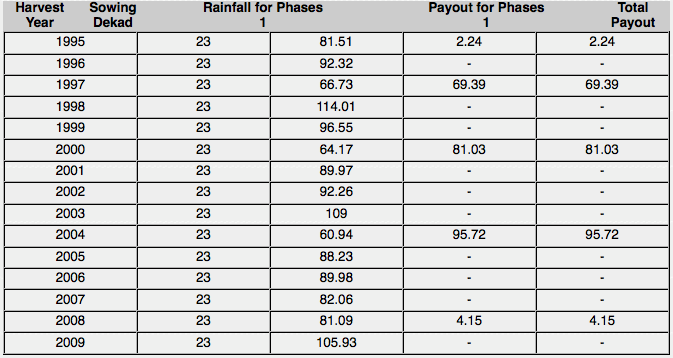
\includegraphics{wiiex1tab.png}}\hfill}

{\scalebox{0.700000}{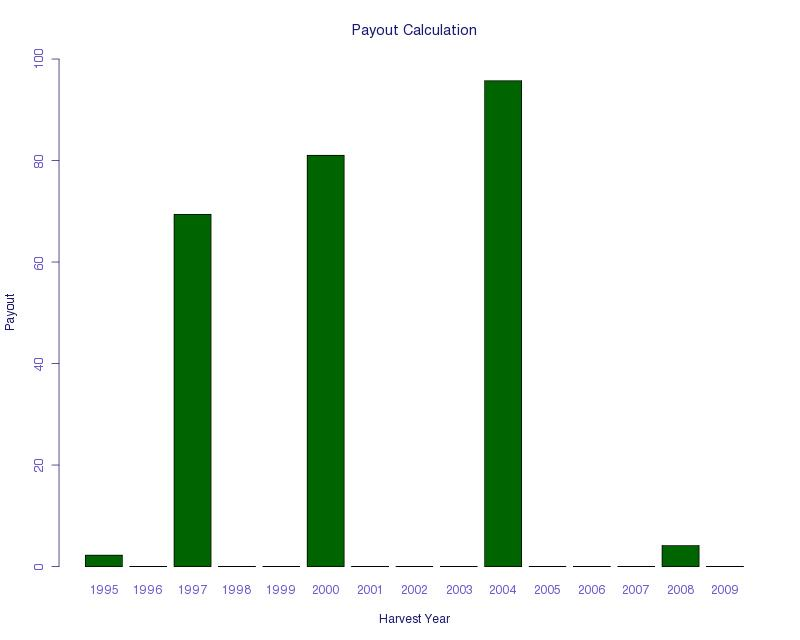
\includegraphics{wiiexgra.png}}\hfill}


\subsubsection{Task 2: Adjusting the drought index based on farmer input}
\label{wiiet/wiiet_usingfarmerinformationanskey:task-2-adjusting-the-drought-index-based-on-farmer-input}\begin{enumerate}
\item {} 
How many payouts would this community have experienced in the last 15 years, if this new index had been used? \textbf{Payouts in nearly all years.} \emph{See table and graph below.}

\item {} 
Is this a realistic index? \textbf{Not really, as it would make the contract extremely expensive.}

\item {} 
What else can be adjusted to create a better index that also addresses the farmers' concerns? \textbf{Exit and Trigger; this will be the main goal of Task 3}

\end{enumerate}

{\scalebox{0.700000}{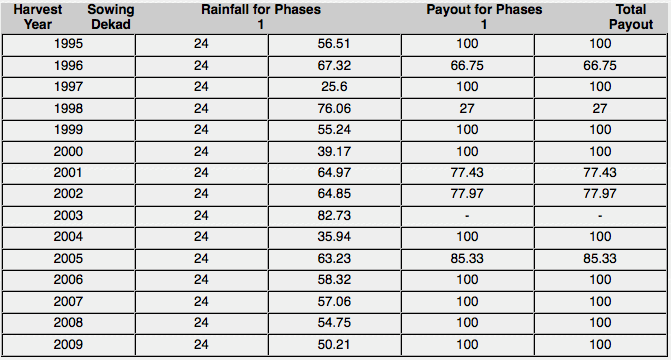
\includegraphics{wiitask2.png}}\hfill}

{\scalebox{0.700000}{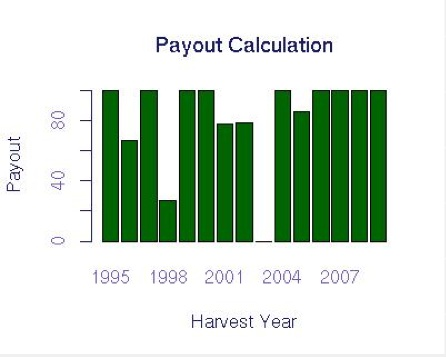
\includegraphics{wit2g.jpg}}\hfill}


\subsubsection{Task 3: Making a More Appropriate Index}
\label{wiiet/wiiet_usingfarmerinformationanskey:task-3-making-a-more-appropriate-index}
\emph{(One suggested index. See example table and graph below)}
\begin{enumerate}
\item {} 
What trigger value have you chosen? \textbf{55}

\item {} 
What exit value have you chosen? \textbf{25}

\end{enumerate}

{\scalebox{0.700000}{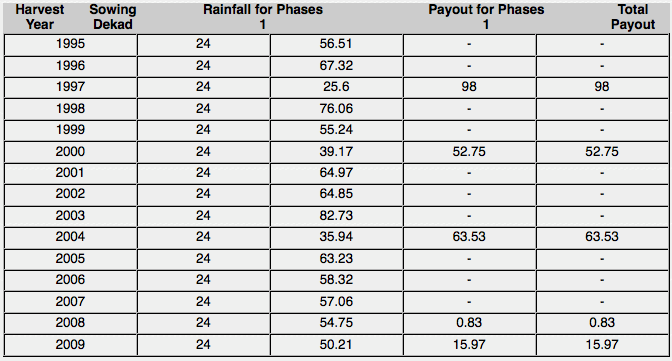
\includegraphics{wt3t.png}}\hfill}

{\scalebox{0.700000}{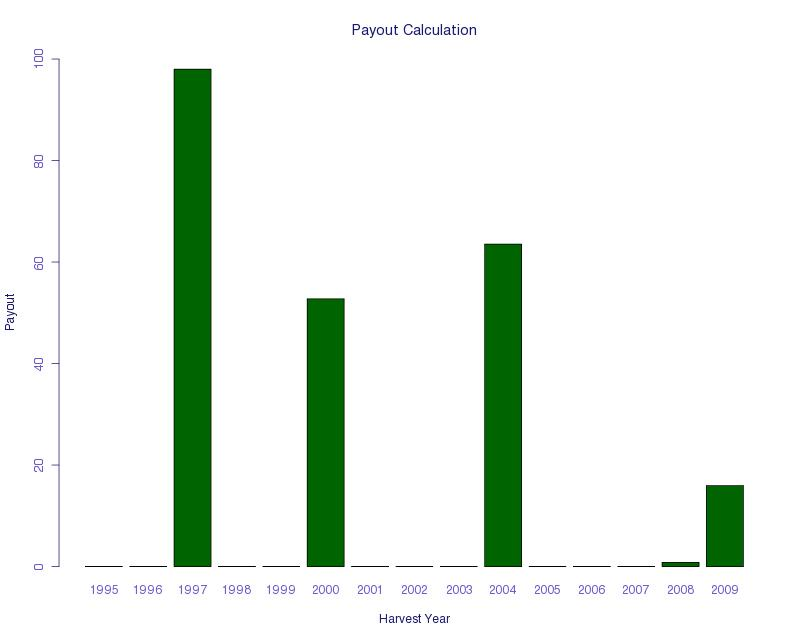
\includegraphics{wt3g.png}}\hfill}

Payout years: 1997, 2000, 2004, 2008, 2009

\textbf{Discussion:}

To remind you of the farmers' input:

Bad years from farmers: 2000, 2004, 2006, 2007, 2009

Very bad years: 2000, 2004, 2009

This index meets many of our design goals. It does not have too many large payments (which would increase the price), and it pays out in the very bad years mentioned by farmers. For most of the very bad years, there is a large payout, except for 2009, which would have had a relatively small payout.

Often, years very far in the past will not be on the farmers' minds during design discussions. Thus, it is valuable to use the discussion and farmer input to focus further on evaluating the more recent payouts.

This index has a few limitations that will need to be discussed with farmers. It provides payouts in 1997 and 2008, which were not mentioned as drought years. From our rainfall data, 1997 is a very bad year. In discussions with experts, 1997 was a year with very low rainfall, so it is likely that it was actually a bad year, and we believe it would be a worthwhile payout.

It also does not provide a payout in 2006, which was mentioned by farmers as a bad year. This is a primary concern. We need to follow up in the next farmer discussion to see if this year was really that bad, and also if it would be acceptable to have a product that would not have paid out in 2006.  Typically, the index cannot be made perfect. The farmer design team must feel comfortable about the amount of mismatch in the contract in order to proceed with implementation.


\subsubsection{Task 4: Farmer discussion follow-up notes}
\label{wiiet/wiiet_usingfarmerinformationanskey:task-4-farmer-discussion-follow-up-notes}\begin{enumerate}
\item {} 
What parameter will you adjust to fulfill the farmers' request? \textbf{Exit}

\item {} 
Will this number be increased or decreased? \textbf{Increase}

\item {} 
Will this result in a more expensive index? Why or why not? \textbf{Yes, more expensive. A full payout occurs when the exit is above the rain by phase. Partial payouts occur when the rain by phase is between the trigger and the exit. When the exit is raised there is potential for more full payouts and larger partial payouts, making the index more expensive.}

\end{enumerate}

One example of the payouts for the index resulting from this process is presented below:

{\scalebox{0.700000}{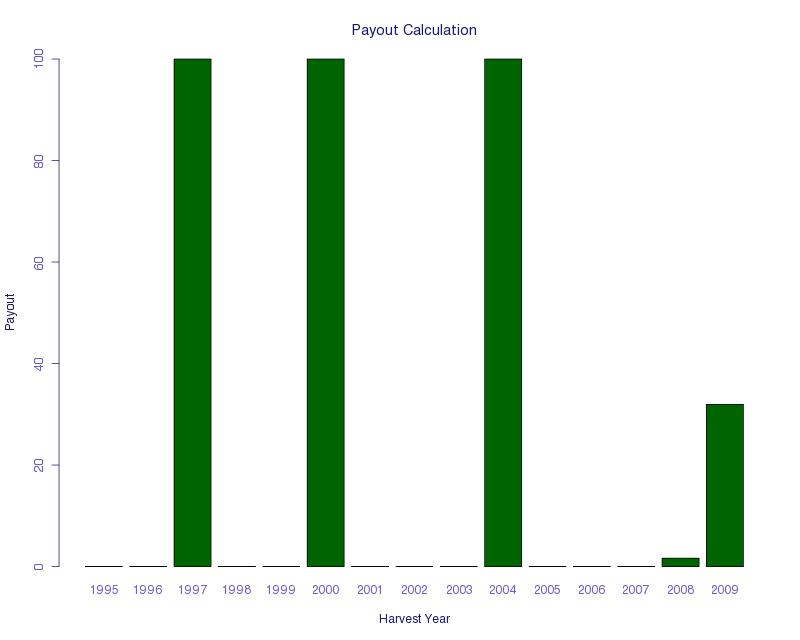
\includegraphics{wt4g.png}}\hfill}


\subsection{WIIET Exercise 2 Answer Key: Influence of Short Datasets on Prices (Advanced Exercise)}
\label{wiiet/wiiet_influenceshortdatasetsanskey:wiiet-exercise-2-answer-key-influence-of-short-datasets-on-prices-advanced-exercise}\label{wiiet/wiiet_influenceshortdatasetsanskey::doc}

\subsubsection{Task 2: Thinking about simulated rainfall}
\label{wiiet/wiiet_influenceshortdatasetsanskey:task-2-thinking-about-simulated-rainfall}
\textbf{Answers}

Does the rainfall in years generated by the rainfall simulator have more variation in rainfall than the historical record or less?  Why or why not? \textbf{More, because the simulator expands the variation to reflect statistical uncertainty in climate}


\subsubsection{Task 3: Applying a simulated rainfall dataset}
\label{wiiet/wiiet_influenceshortdatasetsanskey:task-3-applying-a-simulated-rainfall-dataset}
\textbf{Answers:}

\textbf{Over almost 1,000 years, there are many payouts. See the graph below}

{\scalebox{0.700000}{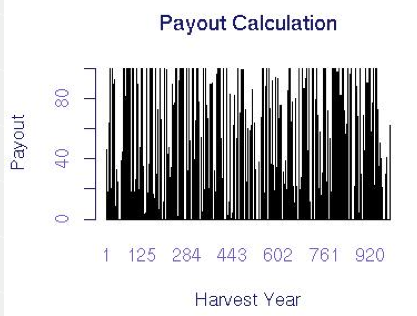
\includegraphics{payouts.png}}\hfill}


\subsubsection{Task 4: Historical verses simulated rainfall data}
\label{wiiet/wiiet_influenceshortdatasetsanskey:task-4-historical-verses-simulated-rainfall-data}
\textbf{Answers}
\begin{enumerate}
\item {} 
Will insurance prices be higher than the risk prices you calculate using WIIET? \textbf{Higher}

\item {} 
Why or why not? \textbf{Real prices are negotiated and include additional costs not modelled by WIIET}

\item {} 
What is the purpose of calculating risk prices using WIIET? \textbf{The purpose of using WIIET for pricing is to learn how changes in risk and analysis approaches influence price.}

\end{enumerate}


\subsubsection{Task 5: Risk Pricing}
\label{wiiet/wiiet_influenceshortdatasetsanskey:task-5-risk-pricing}\begin{enumerate}
\item {} 
Risk Pricing for Historical Rainfall (see below table)
\begin{enumerate}
\item {} 
What is the risk premium of the original contract calculated using the historical data? \textbf{24.7 or 24\%}

\item {} 
What is the average payout? \textbf{16.83}

\item {} 
Why is the premium higher than the average payout? \textbf{Loading/interest on money for payouts}

\end{enumerate}

\end{enumerate}
\begin{figure}[htbp]
\centering

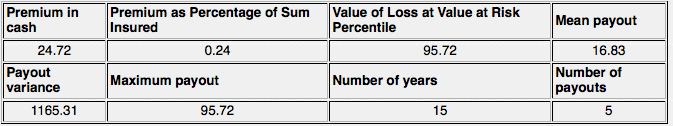
\includegraphics{premium.png}
\end{figure}
\begin{enumerate}
\setcounter{enumi}{1}
\item {} 
Risk Pricing for Simulated Rainfall
\begin{enumerate}
\item {} 
Which payout series has a higher risk price? \textbf{Simulation}

\item {} 
Why? \textbf{First, because it has additional uncertainty due to statistical climate uncertainty. Second, because it includes potential years that do not exist in the historical dataset, but that are likely to occur.}

\item {} 
What is the payout rate for the simulated series (divide the number of payouts by the number of years)? \textbf{363/990=36.6\%}

\item {} 
Is this higher or lower than the 30\% payout rate obtained when using the historical data series? \textbf{Higher than historical burn payout rate}

\item {} 
Why? \textbf{For reason from previous question}

\end{enumerate}

\end{enumerate}
\begin{figure}[htbp]
\centering

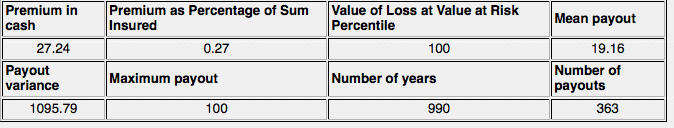
\includegraphics{premium2.png}
\end{figure}

\textbf{Advanced Question:}

Although the mean payout is higher for the simulated payout series (as would be expected), the variance in the payouts is actually lower.  How is this possible and what does it say about the changes in payouts? \textbf{This means that the index and increased variance in the data interact in such a way that there are fewer full payouts but more small payouts, increasing the mean payout but decreasing the variance.}


\subsubsection{Task 6: Length of dataset and risk price of insurance}
\label{wiiet/wiiet_influenceshortdatasetsanskey:task-6-length-of-dataset-and-risk-price-of-insurance}\begin{enumerate}
\item {} 
Is the payout rate (number of payouts/number of years) for the simulated rainfall series using the recent data series higher or lower than that of the simulated rainfall series using the full set of historical data? \textbf{Higher (see table below)}

\item {} 
Why? \textbf{Because the short simulation has additional variation due to the increased statistical uncertainty from the short data series}

\item {} 
Are the mean, variance, and price for the simulated rainfall series using the recent data series higher or lower than that of the simulated rainfall series using the full set of historical data? \textbf{Higher for all}

\item {} 
Why? \textbf{Because the short simulation has additional variation due to the increased statistical uncertainty from the short data series}

\end{enumerate}
\begin{figure}[htbp]
\centering

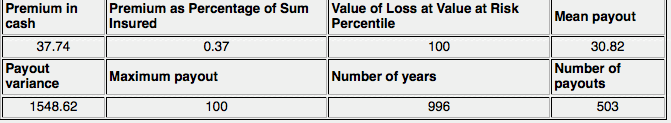
\includegraphics{premium3.png}
\end{figure}

\textbf{Advanced Task:}

\textbf{Questions:}

Can comparison of short and long historical datasets give you the information you got from earlier tasks comparing simulated rainfall? Why or why not? \textbf{The information problems associated with understanding the climate with a short dataseries are not modelled using historical data; a rainfall simulator is required. Because the data series is so short, results from comparisons will be spurious, driven by the luck of the draw from very few years.}
\begin{figure}[htbp]
\centering

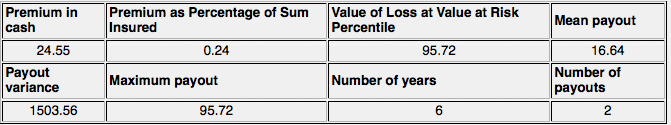
\includegraphics{premium4.png}
\end{figure}


\subsection{WIIET Exercise 3 Answer Key: Moving from Initial Pricing to Market Pricing}
\label{wiiet/wiiet_initialtomarketpricinganskey::doc}\label{wiiet/wiiet_initialtomarketpricinganskey:wiiet-exercise-3-answer-key-moving-from-initial-pricing-to-market-pricing}

\subsubsection{Task 2: Pricing of Historical Rainfall Dataset}
\label{wiiet/wiiet_initialtomarketpricinganskey:task-2-pricing-of-historical-rainfall-dataset}
\textbf{Answers:}
\begin{enumerate}
\item {} 
What is the historical risk price (``premium in cash'')? \textbf{24.72}

\item {} 
How many payouts occur using the historical rainfall dataset? \textbf{5}

\item {} 
What is the average payout? \textbf{16.83}

\item {} 
Does the maximum possible payout occur when using this dataset? \textbf{No.}

\item {} 
Why is the historical risk price higher than the average payout?  \textbf{Because enough money must also be held to account for extreme payouts.}

\item {} 
What is the payout variability? \textbf{1165.31}

\end{enumerate}


\subsubsection{Segment 1: Advanced Statistical Analysis}
\label{wiiet/wiiet_initialtomarketpricinganskey:segment-1-advanced-statistical-analysis}
\textbf{Answers:}
\begin{enumerate}
\item {} 
Why do statistical models provide a good robustness test for our index? \textbf{They elaborate on the uncertainty inherent in the historical dataset. This allows us to test if we've fit our index too closely to the historical dataset.}

\item {} 
What are the benefits of using statistical models in the pricing process? \textbf{They provide a systematic approach for analysis and can be clearly documented.}

\item {} 
What are the limitations of using advanced statistical analysis as a pricing method? \textbf{The results of this analysis will only be as good as the model. Every model has its limitations and cannot account for every scenario that may happen in actuality.}

\item {} 
In what scenario would a statistical model provide the correct price for an insurance package? \textbf{In a world where all the models assumptions were true, the model would provide the correct price of insurance.}

\end{enumerate}


\subsubsection{Task 3: Simulated Rainfall}
\label{wiiet/wiiet_initialtomarketpricinganskey:task-3-simulated-rainfall}
\textbf{Answers}
\begin{enumerate}
\item {} 
What is the simulated rainfall risk price? \textbf{27.24}

\end{enumerate}

2. Is this higher or lower than the historical risk price calculated above?
\textbf{Higher}
\begin{enumerate}
\setcounter{enumi}{2}
\item {} 
What is the average payout? \textbf{19.16}

\item {} 
Does the average payout increase or decrease compared to the historical burn index? \textbf{Increase}

\item {} 
What is the payout variability? \textbf{1095.79}

\item {} 
Does the payout variability increase or decrease compared to the historical burn index? \textbf{Decrease}

\item {} 
Using just this analysis, do these results indicate that your historical burn index is robust? \textbf{Based on just this analysis, most likely this is a fairly robust index. It does not appear to have been over fitted to the 15 years of historical data, as the pricing results are similar to those seen for the historical burn analysis. However, this is an opinion-based question and there is no right answer. Each person/stakeholder may have a different opinion as to how much variation is acceptable, appropriate and within their range of comfort.}

\end{enumerate}


\subsubsection{Segment 2: Sensitivity Tests}
\label{wiiet/wiiet_initialtomarketpricinganskey:segment-2-sensitivity-tests}
\textbf{Answers:}
\begin{enumerate}
\item {} 
Why do insurance and reinsurance companies perform sensitivity tests? \textbf{To provide additional robustness tests for insurance contracts.}

\item {} 
What does it tell you if the price of your index changes dramatically when you perform a sensitivity test? \textbf{That your contract is probably not as robust as it needs to be.  This typically reflects that the contract has been designed too closely to fit the data used in the initial design process.}

\item {} 
How does a robust index perform under sensitivity tests? \textbf{The price, payout frequency, payout variability and average payout may vary slightly, but will still be within a reasonable range of the results you had using your original dataset.}

\end{enumerate}


\subsubsection{Task 4:  Determining Sensitivity to a General Decrease in Rainfall}
\label{wiiet/wiiet_initialtomarketpricinganskey:task-4-determining-sensitivity-to-a-general-decrease-in-rainfall}
\textbf{Answers:}
\begin{enumerate}
\item {} 
What is the risk price for the five percent less rainfall?  \textbf{27.10}

\item {} 
Is this higher or lower than the historical burn risk price? The simulated rainfall risk price? \textbf{Higher; Lower, but about the same.}

\item {} 
How much did your average payout, number of payouts and payout variability change as compared to using the historical rainfall?  \textbf{The simulated rainfall? As compared to the historical rainfall: The average payout increased by 2.17, the number of payouts increased by one, and the payout variability increased by 194.13. As compared to the simulated rainfall: The average payout decreased by 0.16, the payout rate is 3.33 percent higher than when using the simulated rainfall, and the payout variability is 263.65 higher.}

\item {} 
What does this tell you about your index's sensitivity to decreased rainfall? \textbf{Again, this is an opinion-based question and it will depend on how tolerant you are to the risk price being raised a few percentage points and other variations. Overall these results are still very similar to the results we saw when using the historical and simulated rainfall, and it is most likely that the index is not particularly sensitive to this type of overall decrease in rainfall.}

\end{enumerate}


\subsubsection{Task 5: Determining Sensitivity to a Shift Forward in the Rainy Season}
\label{wiiet/wiiet_initialtomarketpricinganskey:task-5-determining-sensitivity-to-a-shift-forward-in-the-rainy-season}
\textbf{Answers:}
\begin{enumerate}
\item {} 
What is the risk price when the rainy season is shifted forward by one day? \textbf{28.36}

\item {} 
Is this higher or lower than the historical burn risk price? The simulated rainfall risk price? \textbf{Higher; higher}

\item {} 
How much did your average payout, number of payouts and payout variability change as compared to using the historical rainfall? \textbf{The simulated rainfall? As compared to historical rainfall: The average payout increased by 3.57, the number of payouts increased by 1, and the payout variability increased by 143.26.  As compared to simulated rainfall: The average payout increased by 1.24, the payout rate is 3.33 percent higher than when using the simulated rainfall, and the payout variability increased by 212.78.}

\item {} 
What does this tell you about your index's sensitivity to a shift forward in the rainy season? \textbf{So far our contract appears to be the most sensitive to a shift forward in the rainy season, however we still only see an increase of a few percentage points in the risk price. This analysis does not reveal any severe danger signs, but because the index was the most sensitive to this shift you may want to be cautious and aware of this as you move forward. As this is an opinion-based question, others may not be as comfortable with this amount of variation and feel that it may be cause for concern, possibly calling for adjustments to be made to address this risk. The reason that this sensitivity check has resulted in the largest impact is because you are effectively adding an additional dry day to every season and removing what is probably a wet day.}

\end{enumerate}


\subsubsection{Task 6: Determining Sensitivity to a Shift to a Later Rainy Season}
\label{wiiet/wiiet_initialtomarketpricinganskey:task-6-determining-sensitivity-to-a-shift-to-a-later-rainy-season}
\textbf{Answers:}
\begin{enumerate}
\item {} 
What is the risk price when the rainy season is shifted back by one day? \textbf{19.62}

\item {} 
Is this higher or lower than the historical burn risk price? The simulated rainfall risk price? \textbf{Lower, lower.}

\item {} 
How much did your average payout, number of payouts and payout variability change as compared to using the historical rainfall?  The simulated rainfall? \textbf{As compared to historical rainfall: the average payout is 3.05 lower, there is the same number of payouts, the payout variance is 431.36 less. As compared to simulated rainfall: The average payout is 5.38 lower, the payout pays out about 3.34\% less frequently, and the payout variance is 361.84 lower.}

\item {} 
What does this tell you about your index's sensitivity to a shift to a later rainy season? \textbf{That this risk is not likely to affect the contract's performance, and is probably not a concern we need to worry about.}

\end{enumerate}


\subsubsection{Segment 4: Moving from Risk Pricing to Market Pricing: using spreadsheets}
\label{wiiet/wiiet_initialtomarketpricinganskey:segment-4-moving-from-risk-pricing-to-market-pricing-using-spreadsheets}

\subsubsection{Task 9: Determining Pricing Parameters}
\label{wiiet/wiiet_initialtomarketpricinganskey:task-9-determining-pricing-parameters}
\textbf{Answers:}
\begin{enumerate}
\item {} 
What is your final value for the additional loading due to uncertainty? \textbf{Results will vary by participant-there is really no correct answer here and many considerations}

\item {} 
What is your final market price? \textbf{Again, results will vary by participant}

\item {} 
What three values does the spreadsheet add together to calculate the final market price? \textbf{The Risk Price (25\%), Administrative and Business Expenses (3\%), and Additional Loading Due to Uncertainty}

\end{enumerate}



\renewcommand{\indexname}{Index}
\printindex
\end{document}
